
% arara: pdflatex
% arara: pdflatex
% arara: pdflatex

% options:
% thesis=B bachelor's thesis
% thesis=M master's thesis
% czech thesis in Czech language
% slovak thesis in Slovak language
% english thesis in English language
% hidelinks remove colour boxes around hyperlinks

\documentclass[thesis=B,czech]{FITthesis}[2019/12/23]

\usepackage[utf8]{inputenc} % LaTeX source encoded as UTF-8

% \usepackage{amsmath} %advanced maths
% \usepackage{amssymb} %additional math symbols

\usepackage{dirtree} %directory tree visualisation
\usepackage{pdfpages}
\usepackage{soul}
\usepackage{varwidth}
\usepackage{minted}
\usepackage{placeins}
\usepackage{flafter}
\usepackage{polyglossia}
\setdefaultlanguage{czech}
\setotherlanguages{english}
\usepackage[backend=biber,style=iso-numeric]{biblatex}

\addbibresource{mybibliographyfile.bib}

\setcounter{biburllcpenalty}{7000}
\setcounter{biburlucpenalty}{8000}
% % list of acronyms
% \usepackage[acronym,nonumberlist,toc,numberedsection=autolabel]{glossaries}
% \iflanguage{czech}{\renewcommand*{\acronymname}{Seznam pou{\v z}it{\' y}ch zkratek}}{}
% \makeglossaries

\newcommand{\tg}{\mathop{\mathrm{tg}}} %cesky tangens
\newcommand{\cotg}{\mathop{\mathrm{cotg}}} %cesky cotangens

% % % % % % % % % % % % % % % % % % % % % % % % % % % % % % 
% ODTUD DAL VSE ZMENTE
% % % % % % % % % % % % % % % % % % % % % % % % % % % % % % 

\department{Katedra teoretické informatiky}
\title{Vícevláknová metoda řazení Timsort}
\authorGN{Daniel} %(křestní) jméno (jména) autora
\authorFN{Blažek} %příjmení autora
\authorWithDegrees{Daniel Blažek} %jméno autora včetně současných akademických titulů
\author{Daniel Blažek} %jméno autora bez akademických titulů
\supervisor{doc. Ing. Ivan Šimeček, Ph.D.}
\acknowledgements{Rád bych upřímně poděkoval svému vedoucímu bakalářské práce, doc. Ing Ivanu Šimečkovi, Ph.D., za jeho cenné rady, odborné vedení a trpělivost.}
\abstractCS{Cílem této práce je zabývat se sekvenčními optimalizacemi algoritmu Timsort a jeho paralelizací pomocí OpenMP. Nově vzniklé algoritmy jsou otestovány a porovnány se základní verzí Timsortu a dalšími vybranými řadícími algoritmy. Toto testování je prováděno na školním serveru STAR určenému k objektivnímu testování paralelních algoritmů. Veškerá implementace je v jazyce C++. }
\abstractEN{The aim of this thesis is to explore the sequential optimizations of the Timsort algorithm and its parallelization using OpenMP. Newly developed algorithms are tested and compared with the base version of Timsort and other selected sorting algorithms. This testing is performed on the school server STAR, designed for objective testing of parallel algorithms. All implementations are in the C++ language.}
\placeForDeclarationOfAuthenticity{V~Praze}
\declarationOfAuthenticityOption{4} %volba Prohlášení (číslo 1-6)
\keywordsCS{timsort, c++, openmp, paralelizace, řadící algoritmus, mergesort, paralelní timsort, optimalizace, řadící algoritmy} 
\keywordsEN{timsort, c++, openmp, parallelization, sorting algorithm, mergesort, paralel timsort, optimalization, sorting algorithms}
% \website{http://site.example/thesis} %volitelná URL práce, objeví se v tiráži - úplně odstraňte, nemáte-li URL práce



\begin{document}



% \newacronym{CVUT}{{\v C}VUT}{{\v C}esk{\' e} vysok{\' e} u{\v c}en{\' i} technick{\' e} v Praze}
% \newacronym{FIT}{FIT}{Fakulta informa{\v c}n{\' i}ch technologi{\' i}}

\begin{introduction}
	%sem napište úvod Vaší práce


%proč je zajímavé se problém zabývat
Řadící algoritmy jsou všude kolem nás. Umožňují nám nejen ukazovat v jakém vztahu jsou různé objekty, ale pomáhají nám v nich i hledat. Ať už to je srovnávání cen v e-shopech a nebo řazení šanonů podle jmen. Zdá se, že řadící algoritmy potřebujeme čím dál tím více, abychom se v tomto komplikovaném světě mohli orientovat.

Nacházení nových optimalizací je proto velmi důležité pro vytváření rychlejších, paměťově efektivnějších a všestrannějších řadících algoritmů. Zároveň je důležité již nalezené optimalizace maximálně zjednodušit. Usnadní se tím implementace, sníží počet možných chyb a je jednodušší provádět důkaz korektnosti optimalizovaného algoritmu.

Tato práce se zabývá možnostmi sekvenčních optimalizací a paralelizací řadícího algoritmu Timsort. Tento algoritmus je založený na algoritmu Mergesort s několika optimalizacemi. Ty například zajišťují, že je Timsort adaptivní řadící algoritmus a zároveň vyžaduje méně paměti než klasický Mergesort. Proto se algoritmy založeny na principech Timsortu využívají například v jazyce Python, Java, Rust a Swift.

V této práci se snažím najít nějaké další potencionální optimalizace. Také zkouším jak by mohla fungovat paralelní verze tohoto algoritmu. Správně implementovaná paralelizace nám umožní dále zrychlit algoritmus za využití více vláken.

%motivace výběru tématu
Při výběru tématu a studiu Timsortu a dalších řadících algoritmů, které se reálně používají v různých jazycích a knihovnách mě zaujalo, jak jsou promyšlené do nejmenšího detailu a že i malá změna algoritmu může udělat obrovský rozdíl pro určitý typ dat.

%popis struktury práce (stručný popis následujících sekcí)
V následující sekci jsou popsány cíle této práce. Dále je vysvětleno, jak algoritmus Timsort funguje a jaké optimalizace se běžně používají. Poté navrhuji, jaké optimalizace lze přidat a nakonec se věnuji jejich implementaci a testování. Na závěr jsou zhodnoceny výsledky testování.
\end{introduction}

\chapter{Cíl práce}
\section{Sekvenční optimalizace algoritmu}
V rámci vylepšení algoritmu je důležitá jejich optimalizace. U řadících algoritmů bývá nejdůležitější jejich rychlost. Dále je důležitá i jejich paměťová složitost. Můžeme optimalizovat obecně celý algoritmus pro všechny vstupy a nebo se zaměřit pouze na vstupy, které dopadají špatně. Také můžeme optimalizovat tím, že zrychlíme některé operace -- například přístup do paměti pomocí lepšího využití cache paměti.


Timsort je navržen tak, aby využíval co nejvíce struktur, které se v datech přirozeně vyskytují. Je tedy velmi těžké naleznout vylepšení samotného algoritmu, které by jej urychlilo. V mé práci se proto snažím upravit algoritmus tak, aby lépe využíval cache paměť.

\section{Paralelizace algoritmu}

Dalším způsobem jak je možné zrychlit algoritmus je jeho paralelizace. Při paralelizaci se program spustí ve více vláknech. Pokud je dobře navržena dojde tím k jeho zrychlení, protože se může vykonávat více částí programu najednou. 
Timsort vynucuje sekvenční chování díky svým invariantům. Cílem je vymyslet různé způsoby jak lze přes tento problém algoritmus paralelizovat.

\section{Testování}

Posledním cílem této práce je otestovat mnou navržené verze algoritmu. Pro zajištění co nejpřesnějších měření bude testování prováděno na školním serveru STAR. Tento server je přímo určen k objektivnímu měření paralelních programů.

\chapter{Analýza a návrh}


\section{Popis algoritmu Timsort}
Algoritmus Timsort je hybridní, adaptivní a stabilní řadící algoritmus se složitostí $ \mathcal{O}(n \log{n}) $ odvozený z Mergesortu a Insertion sortu.\cite{timexplain5} Funguje velmi dobře na datech reálného světa a proto se jeho principy používají v řadících algoritmech pro Pythonu\cite{pythonimpl}, Rustu\cite{rustimpl}, Javě\cite{javaimpl}, V8 (Javascript engine)\cite{v8impl} a Swiftu\cite{swiftimpl}. Pro své dobré používání cache paměti a stabilitu se hodí především na neprimitivní typy\cite{timexplain4}. Zbytek této sekce je založen především na detailním popisu Timsortu jeho tvůrcem Timem Petersem, včetně odůvodnění některých rozhodnutí a příkladů.\cite{timexplain1,timexplain2,timexplain3,timexplain6}

V první části algoritmu se hledají takzvané „natural runs“, což jsou již seřazené části pole. Run může být vzestupný $ a_0 \le a_1 \le a_2 $ nebo ostře klesající $ a_0 > a_1 > a_2 $. Ostře klesající musí být, aby algoritmus zůstal stabilní, neboť se na tento run provede naivní in-place otočení posloupnosti. Stejné hodnoty by se jinak prohodily. 

Dále existuje hodnota \texttt{minRun} určující minimální velikost pro run. Pokud jí run nedosáhne je doplněn dalšími prvky pomocí Binary insertion sortu. V poli s náhodnými daty to tedy znamená, že runy mají stejné délky při slučování, čímž získáme nejmenší nutný počet slučování. 
Navíc využijeme faktu, že pro malá pole je výhodnější použít Insertion sort než Mergesort, kvůli vyšší rychlosti.
Výpočet hodnoty \texttt{minRun} pro $ N < 64 $ je roven $ N $. Pokud je $ N $ násobkem dvěma lze použít hodnoty $ 16,32,64,128 $, které jsou zhruba ekvivalentní. Vyšší hodnoty zpomalují Insertion sort a nižší zpomaluje počet volání funkce slučování. Použití násobku dvěma je důležité, aby slučování runů bylo vyrovnané. Pokud ale $ N $ není násobkem dvěma, je potřeba se zamyslet nad tím, aby se zbytečné neslučovaly velká pole s malými. Proto se jako \texttt{minRun} používá hodnota taková, aby $ \frac{N}{\texttt{minRun}} \in {32,...,65} $ a zároveň aby $ \frac{N}{\texttt{minRun}} $ byla mocnina dvojky, anebo ostře menší než mocnina dvojky, pokud nemůže být přesně mocnina dvojky.

Představme si, že bychom takto nevypočítávali minimální délku runu a použili fixní hodnotu 32. Uvažujme pole o délce 2112 prvků. Pokud jsou data náhodná, dostaneme velmi pravděpodobně 66 runů o délce 32. Sloučení prvních 64 runů bude dokonale vyvážené, avšak poté nastane situace, kdy budeme chtít sloučit runy o velikosti 2048 a 64. To je velmi neefektivní -- je potřeba daleko více porovnání a kopírování dat.

Nyní uvažujme výpočet minimální délky runu, tak je popsán výše. Jako hodnota \texttt{minRun} nám vyjde číslo 33. S náhodnými daty opět velmi pravděpodobně získáme runy právě s minimální délkou - tím pádem jich bude 64. Jelikož je počet runů násobkem dvou, dostaneme jejich vyvážené slučování.

\subsection{Slučovací strategie}
Během hledání runů se může stát, že délky runů mohou být velmi rozdílné. Proto je potřeba organizovat slučování runů. Abychom zachovali stabilitu algoritmu můžeme slučovat pouze runy, které jsou vedle sebe. Uvažujme tedy, že máme 3 runy $ A, B, C $, které chceme sloučit. Máme na výběr $ (A+B)+C $ nebo $ A+(B+C) $. Během slučování je potřeba najít kompromis, kdy ho provést, protože chceme využít dvou protichůdných vlastností. Jednak chceme, aby slučování bylo provedeno co možná nejpozději, abychom mohli využít struktury dat, které mohou přijít později. Zároveň chceme slučování provést co nejdříve, abychom využili dobře cache paměť, protože data byla nedávno použita. Udržování informací o runech také spotřebovává paměť navíc.

Jako dobrý kompromis se ukázalo udržovat dva invarianty na poslední 3 runy na zásobníku. Pro jejich délky $A, B, C$ by pak mělo platit: 
\begin{center}
\begin{varwidth}{\textwidth}
\begin{enumerate}
	\item $ A > B + C $
	\item $ B > C $
\end{enumerate}
\end{varwidth}
\end{center} 
První invariant zajišťuje, že délky runů rostou alespoň tak rychle, jako Fibonacciho čísla. Proto nám stačí malý zásobník i pro velmi velká pole. Druhý invariant zajišťuje, že runy jsou seřazeny podle délek od největší po nejmenší. Tím získáváme dobré slučování, protože slučujeme runy s nejvíce podobnou délkou. Pokud je některý invariant nesplněn, po prvním sloučení se může pořád stát, že invarianty pořád nejsou splněny -- viz příklad. Proto je potřeba toto provádět, dokud invarianty neplatí. 

Pokud je $A \ge B + C$, tak menší z $A$ a $C$ je sloučen s $B$. Pokud je $A=C$, tak je preferováno $C$, z důvodu nedávného použití a tím větší pravděpodobnosti, že je pořád v cache paměti. Pokud tedy jsou poslední 3 záznamy na zásobníku následující: $A=30$, $B=20$ a $C=10$, potom je $B$ sloučeno s C a výsledek na zásobníku vypadá takto: $A=30$, $BC=30$. 

Jak si můžeme všimnout, tak po sloučení v příkladu pořád neplatí invariant číslo dvě a musíme tedy slučovat znovu, dokud nejsou oba invarianty platné.

\subsection{Slučovací algoritmus}
Na slučování se používají dvě metody, které jsou si podobné. Jedna se stará o situaci $ A \le B $ a druhá o $ A > B $. Tyto metody neví jaká je struktura dat, avšak při sloučení se dá zjistit, když jedna slučovaná strana vyhrává častěji. 

Nejprve se porovná první pár prvků. Při každém porovnání se počítá, který run vyhrál kolikrát v řadě. Pokud tento počet dosáhne hodnoty \texttt{minGallop}, změní se klasické slučování na galloping mód. Při gallopingu módu se hledá v $ B $, kam patří \texttt{A[0]} a překopírují se všechny prvky před tímto bodem. Poté se hledá v $ A $, kam patří \texttt{B[0]} a přesune se zase celý blok prvků. Takto se pokračuje a střídá, dokud nalezené shluky jsou větší než hodnota \texttt{minGallop}. Poté se zas vracíme ke klasickému slučování po jednom páru. 


Jedním z vylepšení přechodu do galloping módu, které Timsort využívá, je nepoužívat pořád stálý \texttt{minGallop} při vstupu do slučovacích funkcí, ale upravovat jeho hodnotu na základě předchozích dat. Funkce \texttt{merge\_lo} a \texttt{merge\_hi} tedy \texttt{minGallop} zvětšují či zmenšují v závislosti na tom, jestli se vyplácí nebo ne. 

\subsection{Slučovací paměť}
Slučovací algoritmus je navržen tak, aby potřeboval co nejméně paměti a byl co nejrychlejší. Byla proto zvolena varianta, kde je potřeba $ \textrm{min}(A,B) $ paměti. Přestože existují in-place slučovací algoritmy, nebyly vybrány, protože jsou příliš složité a pomalé pro praktické využití. 

Pokud je $ A < B $ (funkce \texttt{merge\_lo}), zkopíruje se $ A $ do pomocného pole a začne se slučovat s $ B $ na původní místa $ A $. Na konci případně dokopírujeme zbytek pomocného pole či $ B $ jako v běžném Mergesortu. Pokud je $ A > B $ (funkce \texttt{merge\_hi}) algoritmus funguje obdobně, se změnou, že do pomocného pole zkopírujeme $ B $ a slučujeme z prava doleva –- na původní místo B. Pro $ A = B $ lze využít obě funkce.

Abychom ještě snížili velikost pomocného pole, vyhledá se, kde první prvek $ B $ skončí v $ A $ a kde poslední prvek $ A $ skončí v  $ B $. Stačí nám pak sloučit prvky mezi těmito body. Ostatní už jsou na svém místě. Toto o trochu něco zpomalí algoritmus pro náhodná data, avšak může velmi zrychlit pokud náhodná nejsou. 


\subsection{Galloping}

Galloping neboli exponenciální vyhledávání je technika podobná binárnímu vyhledávání. Je v Timsortu využívána, protože může ve vybraných případech překonat binární vyhledávání, když je hledaný prvek blízko začátku pole. Exponenciální vyhledávání pracuje v časové složitosti $ \mathcal{O}(\log{i}) $, kde $ i $ je index prvku, zatímco binární vyhledávání je v $ \mathcal{O}(\log{n}) $, kde $ n $ je počet prvků v poli.\cite{exponentialsearch}

Předpokládejme bez újmy na obecnosti, že run $ A $ je kratší než run $ B $. V galloping módu porovnáváme prvek \texttt{A[0]} s prvky \texttt{B[0], B[1], B[3], B[7], \ldots, B[$ 2^j - 1 $]}, dokud nenajdeme hodnotu $ k $ takovou, že $ \texttt{B[$ 2^{k-1} - 1 $]} \le \texttt{B[$ 2^k - 1 $]} $. Toto vyžaduje $ \log{B} $ porovnání.

Po nalezení takového $ k $ se region nejistoty zredukuje na $ 2^{k-1}-1 $ za sebou jdoucích prvků a binární vyhledávání potřebuje přesně $ k-1 $ porovnání pro nalezení správné pozice. Poté zkopírujeme všechny prvky z $ B $ do toho bodu a bod \texttt{A[0]}. Nezáleží na tom, kde \texttt{A[0]} patří v $ B $, kombinace gallopingu a binárního vyhledávání toto místo najde za méně než $ 2*\log{B} $ porovnání.

Při použití binárního vyhledávání bychom našli správnou pozici pro \texttt{A[0]} v $ B $ nejpozději za $ \textrm{ceiling}(\log{(B + 1)}) $ porovnání. Na rozdíl od toho galloping mód může najít pozici rychleji, zejména pokud je prvek blíže začátku pole.

Pokud jsou data náhodná a runy mají stejnou délku, pak \texttt{A[0]} patří do \texttt{B[0]} v 50\% případů, do \texttt{B[1]} v 25\% případů atd. Vyhrávající subrun o délce $B$ má tedy pravděpodobnost pouze $ \frac{1}{2^{k+1}} $. Delší vyhrávající subruny jsou tedy extrémně nepravděpodobné.


Pokud ovšem data mají nějakou strukturu nebo obsahují mnoho duplikátů, mají dlouhé vyhrávající subruny daleko větší pravděpodobnost. Snížení počtu porovnání z $ \mathcal{O}(B) $ na $ \mathcal{O}(log{} B) $ je v těchto případech velmi výhodné.

Galloping mód v Timsortu je kompromis, který spočívá v tom, že pokud není dlouhý vyhrávající subrun, tak rychle ukončí a přepne na slučovací mód. Pokud je dlouhý vyhrávající subrun, tak je poté galloping mód velmi efektivní. Tímto způsobem se snaží optimalizovat proces slučování a snížit počet nutných porovnání.


Nicméně galloping má i své nevýhody. Zvyšuje například režii na porovnání, což může ve výsledku zpomalit celý algoritmus, pokud není dobře vyvážen s běžným slučováním.
Galloping může také potřebovat více porovnání než obyčejné lineární prohledávání.
Pokud \texttt{A[0]} patří před \texttt{B[0]}, pak galloping i lineární prohledávání potřebují 1 porovnání. Galloping ovšem vyžaduju navíc i volání funkce. Pokud \texttt{A[0]} patří přímo před \texttt{B[1]}, pak galloping i lineární prohledávání vyžadují 2 porovnání. Třetí porovnání galloping je s prvkem \texttt{B[3]} a pokud \texttt{A[0]} patří před něj, pak musí galloping ještě zjistit jestli patří na \texttt{B[2]} nebo \texttt{B[3]}. Tím pádem potřebuje 4 porovnání. Pokud ale prvek patřil na \texttt{B[2]}, pak lineární prohledávání potřebuje pouze 3 porovnání. Galloping tedy potřeboval o 33\% více porovnání a to je obrovský rozdíl, zejména pokud je porovnávací funkce pomalá. Toto můžeme vidět v tabulce \ref{tab:tab1}.


\begin{table}\centering
	\caption[Porovnání počtu porovnání galloping a lineárního prohledávání]{Porovnání počtu porovnání galloping a lineárního prohledávání}\label{tab:tab1}
 	\begin{tabularx}{1\textwidth}{|>{\centering\arraybackslash}X||>{\centering\arraybackslash}X||>{\centering\arraybackslash}X|>{\centering\arraybackslash}X|>{\centering\arraybackslash}X|}\hline
 		index v $ B $ kam patří \texttt{A[0]}		& počet \mbox{porovnání} \mbox{lineárního} \mbox{prohledávání}		& počet \mbox{porovnání} \mbox{gallopingu}	& počet \mbox{porovnání} \mbox{binárního} \mbox{vyhledávání} & celkem \mbox{porovnání} \mbox{gallopingu}	\tabularnewline \hline \hline
 				0 & 1 & 1 & 0 & 1		\tabularnewline \hline
 		 		1 & 2 & 2 & 0 & 2		\tabularnewline \hline
 		 		2 & 3 & 3 & 1 & 4		\tabularnewline \hline
 		 		3 & 4 & 3 & 1 & 4		\tabularnewline \hline
 		 		4 & 5 & 4 & 2 & 6		\tabularnewline \hline
 		 		5 & 6 & 4 & 2 & 6		\tabularnewline \hline
 		 		6 & 7 & 4 & 2 & 6		\tabularnewline \hline
 		 		7 & 8 & 4 & 2 & 6		\tabularnewline \hline
 		 		8 & 9 & 5 & 3 & 8		\tabularnewline \hline
 		 		9 & 10 & 5 & 3 & 8		\tabularnewline \hline
 		 		10 & 11 & 5 & 3 & 8		\tabularnewline \hline
 		 		11 & 12 & 5 & 3 & 8		\tabularnewline \hline
 		 		\multicolumn{5}{|c|}{\ldots} \tabularnewline \hline
 	\end{tabularx}
\end{table}



Obecně potřebuje lineární prohledávání $i + 1$ porovnání a galloping potřebuje $2*\textrm{floor}(\log{i})+2$ porovnání. Galloping nevyhraje dokud je $i=6$ a dokonce prohraje pokud je $i=2$ a $i=4$. Jelikož v náhodných datech očekáváme malou hodnotu $ i $, mohlo by toto Timsort velmi zpomalit. Proto je jako počáteční hodnota \texttt{minGallop} zvolena právě hodnota 7. I přestože se v náhodných datech může přepnout do galloping módu, je velmi pravděpodobné, že se z něj zase velmi rychle přepne pryč. Pokud však jsou data gallopingu nakloněna, je hodnota 7 zase zbytečně velká a proto si Timsort tuto hodnotu mění na základě již seřazených dat.


Takto funguje galloping mód ve funkci \texttt{merge\_lo}. Obdobně funguje i ve funkci \texttt{merge\_hi} s tím rozdílem, že se hledá od konce. Tím ušetříme spoustu porovnání neboť chceme začínat co nejblíže hledanému prvku. Proto mají tyto funkce parametr hint, který určuje, kde se má začít.


Ve výsledku galloping může zrychlit algoritmus zejména v případech, kdy můžeme využít kopírování větších částí pole. V jiných případech však může způsobit zpomalení, pokud se často přechází mezi módy slučování. Implementace galloping módu také zvyšuje složitost kódu Timsortu, což může vést ke stížení pochopení a k vyšší pravděpodobnosti chyb v implementaci. I přes tyto potenciální komplikace je galloping v Timsortu často užitečný pro zrychlení algoritmu v určitých situacích. Je tedy důležité uvažovat jaká data budeme chtít řadit a podle toho zvážit jestli se galloping vyplatí použít, nebo ne.

\section{Návrh optimalizací}

Algoritmus Timsort obsahuje následující části -- hledání runů a slučování s gallopingem. U hledání runů pravděpodobně optimalizace moc neobjevíme -- samotné procházení je $ \mathcal{O}(n) $, pokud je run o délce $ r $ ostře klesající, otočíme ho za $ \frac{r}{2} $, což rychleji také nepůjde. Máme tedy na výběr jestli run budeme procházet zleva do prava nebo z prava do leva. Další šance na zrychlení u hledání runu by mohla být například změna řadícího algoritmu pro doplnění minimální velikosti runu. 

U slučování je prostor pro optimalizace největší. Hodlám se zajímat i o optimalizace, které algoritmus zrychlí i za cenu vyšší potřeby paměti.

\subsection{Slučování více runů}
Místo toho, abychom slučovali pouze dva sousední runy, můžeme zkusit optimalizovat Timsort tak, aby slučoval více runů najednou. Tato optimalizace by mohla zvýšit rychlost algoritmu, protože by mohla snížit počet nutných sloučení a využít efektivněji cache procesoru.\cite{3merge1} Zároveň hrozí, že algoritmu bude pomalejší, kvůli většímu počtu porovnání.\cite{3mergeresponse,kwaymergemax} Nevýhodou je potřeba větší paměti pro ukládání runů, protože nové invarianty by byly komplikovanější a měly by tím daleko větší režii. Další nevýhodou je ztráta gallopingu, který se u jednoduchého rozšíření popsaného níže nevyplatí. 

Algoritmus slučování dvou runů můžeme jednoduše rozšířit na slučování tří runů tak, že porovnávat tři hodnoty mezi sebou a nejmenší uložíme do výsledku. Jakmile jeden run dojde na konec, použijeme na zbytek obyčejné slučování dvou runů. Obdobně lze rozšířit pro slučování ještě více runů. 

Runy, jejichž počet je mocninou čtyř, můžeme slučovat ještě jiným způsobem. Například pro slučování čtyř runů lze použít sloučení dvakrát dvou runů do pomocného pole a poté sloučení těchto dvou runů zpět do původního pole. Tím ušetříme kopírování výsledků z dočasného pole do původního. Navíc protože ve skutečnosti používáme pouze slučování dvou runů, můžeme využít implementace z Timsortu, která obsahuje i galloping.

Sloučením více runů najednou můžeme teoreticky získat zrychlení.\cite{kwaymergemax} Řadící algoritmy používající $k$ slučování polí najednou nazýváme k-way mergesort. Ačkoliv asymptotická složitost je $ \mathcal{O}(n*\log{n}) $, při podrobnější analýze k-way mergesortů\cite{analysiskmerge} zjistíme následující: 
\begin{center}
Pro $ k = 2 $: $ \frac{n}{2}*2 + \frac{n}{4}*4 + ... + 1 * n = n * \log_2{n} $,
\\pro $ k = 3 $: $ 2*\frac{n}{3}*3 + 2*\frac{n}{9}*9 + ... + 2 * 1 * n = 2*n * \log_3{n} $.
\end{center}
Násobení číslem 2 u $ k = 3$ je způsobeno potřebným počtem porovnání pro zjištění minima.
Obecně tedy lze říct, že pro k-way mergesort platí:\linebreak $ \textrm{počet\_porovnání\_k\_prvků}*n*\log_k{n} $. 
Můžeme najít naivně minimum ve všech $k$ polích. Tím by bylo porovnání k prvků za $ k - 1 $. Můžeme však využít haldu a nebo loser tree získat tak porovnání prvků za $ \mathcal{O}(\log{k}) $.\cite{kwaymerge}

K-way merge se využívá u tzv. external sortů, kde se celá data nevejdou do RAM paměti počítače. Při slučování více polí najednou a tím omezíme přístup do pomalejší externí paměti jako jsou pevné disky.\cite{externalsort} Stejnou výhodu bychom mohli získat i u využívání cache paměti.

\subsection{Timsort s detekcí runů od konce}
Klasický Timsort prochází pole od začátku a hledá runy. Následně je postupně slučuje do jednoho seřazeného pole. Jedna z možných optimalizací je hledat runy procházením pole od zadu. Tento způsob procházení je implementován v jazyce Rust s odůvodněním, že častěji nastává slučování zleva doprava. Při srovnávání slučování právě toto údajně vyšlo lépe a proto je výhodnější hledá runy od konce pole.\cite{rustimpl} Je možné, že pokud ke zrychlení dojde, tak může záležet také na vstupních datech.

\section{Paralelizace Timsortu}


\subsection{První návrh}
Paralelní hledání runů lze provést tak, že rozdělíme pole na menší části, které budou zpracovávány různými vlákny. Každé vlákno pak bude zodpovědné za seřazení své části pole. Hlavní vlákno nakonec provede ještě jednou Timsort a tím bude pole seřazené. Jelikož je Timsort adaptivní a identifikuje runy, tak poslední řazení bude ve výsledku pouze sloučení seřazených částí. Protože spouštění vláken má svoji režii, je potřeba rozdělit pole na tak velké části, aby se vyplatilo jednotlivá vlákna spouštět. V případě malých polí by jinak mohla být paralelní verze výrazně pomalejší. Dále je potřeba brát v potaz kolik vláken může procesor zpracovávat. Velkou výhodou je velmi jednoduchá implementace pomocí OpenMP.\cite{openmp1}

\subsection{Druhý návrh}
Druhou možností paralelizace lze provést tak, že každé vlákno sloučí dvojici runů a výsledné sekvence se následně sloučí ve vyšších úrovních. Velkou nevýhodou je potenciální nerovnoměrné zatížení vláken, pokud délky runů nejsou vyvážené. Navíc je třeba zajistit správnou synchronizaci a koordinaci mezi vlákny. Tato možnost paralelizace je proto pravděpodobně horší a navíc komplikovanější. 

\subsection{Třetí návrh}
Třetí možností paralelizace je inspirována implementací paralelního Timsortu od Saurabha Sooda\cite{soodparallel} a je velmi podobná druhé možnosti paralelizace. Na rozdíl od předchozího návrhu budeme během slučování runů udržovat pole obsahující informace o všech runech. Toto pole bude pro všechny spuštěné funkce vypadat stejně, ale prvky se v runech mohou prohazovat. Jako první krok je potřeba nalézt všechny runy. Poté uvažujeme pole s runy jako pole prvků, které chceme seřadit pomocí obyčejného Mergesortu. Rozdělujeme a rekurzivně voláme funkci, dokud nemáme pouze jeden run. O něm už víme, že je seřazený. Následně pak slučujeme dvojice těchto runů. Výhodou je poměrně jednoduchá implementace velmi podobná Mergesortu s možností jednoduché paralelizace volaných rekurzivních funkcí pomocí direktivy task z OpenMP.



\chapter{Realizace}
Veškerý kód je napsán v jazyce C++. Funkce se volají stejně jako řadící funkce ve standardní C++ knihovně -- pomocí iterátorů a nepovinné porovnávací funkce. Jako výchozí porovnávací funkce je použita \texttt{std::less<>()}. 



\begin{minted}[linenos,breaklines]{c++}
// Příklad volání Timsortu
std::vector<int> numbers = {5, 3, 6, 8, 1, 2, 3};
timsort(numbers.begin(), numbers.end());
timsort(numbers.begin(), numbers.end(), std::greater<>());
\end{minted}


Realizoval jsem tyto algoritmy:
\begin{itemize}
	\item Klasický Timsort
	\item Timsort s vyhledáváním runů od konce
	\item Timsort s 2-way, 3-way a 4-way merge funkcí bez invariantů slučující iterativně a rekurzivně
	\item Dva paralelní Timsorty pomocí OpenMP 
	\item Dva paralelní Mergesorty pomocí OpenMP s různými slučovacími funkcemi
\end{itemize}

\section{Realizace klasického Timsortu}
Algoritmus jsem se pokusil co nejvíce přiblížit původní implementaci pro Python. Ta využívá galloping a šetří maximum paměti při slučování. Jako základ posloužila implementace v Pythonu\cite{pythonimpl} a v Javě\cite{javaimpl}. Tato verze Timsortu je k nalezení v souboru \texttt{timsort.hpp}.

\subsection{Pomocná struktura Slice}
Tato struktura ukládá informace o runu. První proměnná index obsahuje iterátor ukazující na první prvek runu. Proměnná length pak udržuje informaci o délce runu. 

\begin{minted}[linenos,breaklines]{c++}
// Struktura Slice
template <class It>
struct Slice {
    It index;
    int length;
};
\end{minted}

\subsection{Třída TimSort}

Tato třída udržuje všechny potřebné proměnné k tomu, aby Timsort mohl fungovat. Má také na starosti hledání runů a jejich následné slučování. Požaduje 2 template argumenty -- první \texttt{It} je typ iterátoru a druhý \texttt{Compare} je typ porovnávací třídy.
Dále obsahuje následující proměnné:

\paragraph{\texttt{runs}}{pole používané jako zásobník obsahující informace o runech}
\paragraph{\texttt{runsLen}}{aktuální velikost zásobníku \texttt{runs}}
\paragraph{\texttt{tmp\_}}{vektor sloužící jako dočasné pole při slučování}
\paragraph{\texttt{index}}{iterátor ukazující na první prvek aktuálně zpracovávaného runu}
\paragraph{\texttt{first}}{iterátor ukazující na první prvek řazeného pole}
\paragraph{\texttt{last}}{iterátor ukazující na poslední prvek řazeného pole}
\paragraph{\texttt{comp}}{porovnávací funkce}
\paragraph{\texttt{length}}{celková délka řazeného pole}
\paragraph{\texttt{minGallop}}{hodnota podle, které se určuje přechod mezi gallopingem a běžným slučováním, na začátku nastavena na 7, poté se upravuje podle dat}
\paragraph{\texttt{minRun}}{minimální velikost runu}

A následující metody:

\paragraph{\texttt{gallop\_left}}{hledá zleva kam patří hledaný prvek a vrátí jeho index}
\paragraph{\texttt{gallop\_right}}{hledá zprava kam patří hledaný prvek a vrátí jeho index}
\paragraph{\texttt{merge\_lo}}{slučuje prvky obyčejným slučování a případně přejde do gallopingu, paměťově efektivní pokud je první run kratší}
\paragraph{\texttt{merge\_hi}}{slučuje prvky obyčejným slučování a případně přejde do gallopingu, paměťově efektivní pokud je druhý run kratší}
\paragraph{\texttt{merge\_at}}{sloučí run $ i $ a $ i + 1 $, rozhodne kolik prvků je už na správném místě a zvolí lepší variantu z \texttt{merge\_lo} a \texttt{merge\_hi}}
\paragraph{\texttt{binary\_insertion\_sort}}{doplní chybějí část run pomocí Binary insertion sortu}
\paragraph{\texttt{compute\_min\_run}}{vypočítá \texttt{minRun} aby počet runů byl ostře nižší nebo rovnu mocnině dvojky v rozmezí 32 až 64, případně vrátí délku pole pokud je menší než 64}
\begin{minted}[linenos,breaklines]{c++}
// výpočet proměnné minRun
int compute_min_run(int n) {
    int r = 0;           /* becomes 1 if any 1 bits are shifted off */
    while (n >= 64) {
        r |= n & 1;
        n >>= 1;
    }
    return n + r;
}
\end{minted}
\paragraph{\texttt{find\_run}}{nalezne další run, pokud je seřazen opačně, tak ho otočí a pokud je krátký, tak ho doplní na velikost \texttt{minRun}}
\paragraph{\texttt{sort}}{jediná veřejně přístupná metoda třídy, započne seřazení zadaného pole, kontroluje invarianty}\\[10pt]

\noindent Dále jsou mimo třídu dvě obalovací funkce, které zařizují stejné volání jako má \texttt{std::sort}.

\begin{minted}[linenos,breaklines]{c++}
// obalovací funkce Timsortu s porovnávací funkcí
template <class It, class Compare>
void timsort(It first, It last, Compare comp) {
    TimSort<It, Compare> tim(first, last, comp);
    tim.sort();
}

//obalovací funkce Timsortu bez porovnávací funkce
template <class It>
void timsort(It first, It last) {
    timsort<It, decltype(std::less<>())>(first, last, std::less<>());
}
\end{minted}

\subsection{Hledání runů}
O hledání runů se stará metoda \texttt{find\_run}. Ta porovná první a druhý prvek aktuálního runu a rozhodne jestli jde o klesající run nebo neklesající. Jakmile porovná s prvkem, který poruší sekvenci, tak klesající run naivně otočí a v případě, že délka runu není dostatečná, doplní ho na velikost \texttt{minRun} pomocí metody \texttt{binary\_insertion\_sort}. Nakonec run uloží na stack \texttt{runs}.

\subsection{Slučování runů}
Slučování začíná v metodě \texttt{sort}. Ta nejprve najde run pomocí \texttt{find\_run} a poté kontroluje stav invariantů. V případě, že je některý z invariantů porušen, zavolá \texttt{merge\_at} a příslušné runy spojí. Pokud invarianty nejsou porušeny hledá další run, dokud nedojde na konec pole. Až se nalezne poslední run, začnou se všechny runy spojovat do jednoho. Tím nám vznikne seřazené pole.

\begin{minted}[linenos,breaklines]{c++}
// metoda sort ve třídě TimSort
void sort() {
    while (index != last) {
        find_run();
        while (runsLen > 1) {
            int n = runsLen - 2; //check invariants
            if ((n > 0 && runs[n - 1].length <= runs[n].length + runs[n + 1].length) ||
                (n > 1 && runs[n - 2].length <= runs[n - 1].length + runs[n].length)) {
                if (runs[n - 1].length < runs[n + 1].length)
                    --n;
            }
            else if (n < 0 || runs[n].length > runs[n + 1].length) {
                break;
            }
            merge_at(n);
        }
    }

    // merge remaining
    while (runsLen > 1) {
        int n = runsLen - 2;
        if (n > 0 && runs[n - 1].length < runs[n + 1].length)
            --n;
        merge_at(n);
    }
}
\end{minted}

Slučování tedy postupuje dál do metody \texttt{merge\_at}. Ta vytvoří nový run ze zadaného a z runu co následuje. Pokud byl zadán třetí run na stacku, je potřeba první posunout na místo druhého, aby nevznikla mezera. Poté najde kolik prvků z prvního runu je už na svém místě a kolik prvků z druhého runu je na svém místě a ignoruje je. Na zbytek zavolá \texttt{merge\_lo}, pokud je délka prvního runu menší nebo rovna délce druhého runu, jinak zavolá \texttt{merge\_hi}.

Pokračujeme do metod \texttt{merge\_lo} a \texttt{merge\_hi}. Ty jsou si velice podobné. \texttt{Merge\_lo} překopíruje první run do pomocného pole a poté začne porovnávat druhý run s pomocným polem a vkládat výsledné prvky zleva na místo prvního runu. \texttt{Merge\_hi} překopíruje druhý run a vkládá výsledné prvky od konce. Metody fungují i pokud jsou délky opačně než jsem specifikoval na konci minulého odstavce. Přijdeme tím ale o jistotu, že na dočasné pole je potřeba pouze $ \textrm{min}(a,b) $ paměti, kde $a $ je délka prvního runu a $b$ druhého.

V těchto metodách probíhá slučování klasickou metodou, kde porovnáme dva prvky a menší z nich uložíme do výsledku. Pokud ovšem jeden vyhraje víckrát než je hodnota \texttt{minGallop}, přepne se do galloping módu, kde kopírujeme celý blok dat na správné místo. Jakmile je velikost tohoto bloku menší než \texttt{minGallop}, přepne se do klasického slučování. Přechody mezi těmito módy tedy určuje proměnná \texttt{minGallop}. Tyto funkce také tuto proměnnou zvyšují, či snižují v závislosti na tom jak často se módy přepínají.

\subsection{Galloping}

O galloping se starají dvě metody -- \texttt{gallop\_left} a \texttt{gallop\_right}. Jak již název napovídá, tak \texttt{gallop\_left} začíná zleva a \texttt{gallop\_right} zprava. Jinak jsou téměř identické. Popíši proto pouze metodu \texttt{gallop\_left}. 

Jak můžeme vidět v ukázce jejího kódu, tak přijímá parametr \texttt{\_first}, odkazující na první iterátor pole, ve které chceme galloping použít. Dále zde najdeme parametr \texttt{key} určující prvek, kterému chceme nalézt místo v poli. Třetí parametr je \texttt{len} určující délku prohledávaného pole a poslední parametr \texttt{hint} určuje na jakém indexu má galloping začít. 

V samotné metodě nalezneme proměnné \texttt{ofs} a \texttt{lastOfs}, které určují region ve kterém se následně má provést binární vyhledávání. Prvním krokem galloping algoritmu je rozhodnout jestli je hledaný prvek vlevo nebo vpravo od počátečního místa určené parametrem \texttt{hint}. Poté stačí najít region \texttt{[lastOfs, ofs)} ve kterém se hledaný prvek nachází. V tomto regionu na konci vyhledáme prvek pomocí binárního vyhledávání.



\begin{minted}[linenos,breaklines]{c++}
//metoda gallop_left ve třídě TimSort
int gallop_left(const It & _first, T key, int len, int hint) {
    int lastOfs = 0;
    int ofs = 1;
    if (comp(*(_first + hint), key)) { // key > a[base + hint]
        // Gallop right until a[base+hint+lastOfs] < key <= a[base+hint+ofs]
        int maxOfs = len - hint;
        while (ofs < maxOfs && comp(*(_first + (hint + ofs)), key)) {
            lastOfs = ofs;
            ofs = (ofs << 1) + 1;
            if (ofs <= 0)   // int overflow
                ofs = maxOfs;
        }
        if (ofs > maxOfs)
            ofs = maxOfs;
        lastOfs += hint;
        ofs += hint;
    } else { // key <= a[base + hint]
        // Gallop left until a[base+hint-ofs] < key <= a[base+hint-lastOfs]
        int maxOfs = hint + 1;
        while (ofs < maxOfs && !comp(*(_first + (hint - ofs)), key)) {
            lastOfs = ofs;
            ofs = (ofs << 1) + 1;
            if (ofs <= 0)   // int overflow
                ofs = maxOfs;
        }
        if (ofs > maxOfs)
            ofs = maxOfs;
        int tmp = lastOfs;
        lastOfs = hint - ofs;
        ofs = hint - tmp;
    }
    /*
     * We now know that a[b + lastOfs] < key <= a[b + ofs] is true. Do a binary
     * search, to find exact position.
     */
    lastOfs++;
    // binary search
    It pos = std::lower_bound(_first + lastOfs, _first + ofs, key, comp);
    return pos - _first;
}
\end{minted}

\section{Slučování více runů najednou (k-way merge)}


Všechny zde popsané algoritmy jsou k nalezení v souboru \texttt{merging.hpp}. Nejprve jsem naimplementoval vylepšný rekurzivní Mergesort (\texttt{merge\_2\_sort}). Vylepšení spočívá v použití Insertion sortu pro $n < 32$, podobně jako u Timsortu. Poté jsem se implementoval rekurzivní 3-way (\texttt{merge\_3\_sort}) a 4-way (\texttt{merge\_4b\_sort}) mergesort. 2-way mergesort jednoduše rozšíříme na 3-way mergesort tím, že přidáme přídáme hledání minima třetího pole a jakmile jedno pole celé projdeme, tak se problém redukuje na 2-way slučování u kterého stačí zavolat správné parametry. Obdobně lze rozšířit 3-way mergesort na 4-way. U mých k-way mergesortů jsem zůstal u naivního hledání minima ve všech $ k $ polích. Pro větší $k$ toto však nelze použít z důvodu dlouhého a nepřehlednému kódu a také proto, že velký počet potřebných porovnání začne algoritmus velmi zpomalovat způsobem popsaným v analýze. V následující ukázce si můžeme povšimnout ještě funkce \texttt{check\_small\_and\_sort}, která pouze kontroluje délku pole a pokud je dostatečně malé, tak ho seřadí pomocí Binary insertion sortu.



\begin{minted}[linenos,breaklines]{c++}
//slučovací funkce 2-way merge
template <class It, class Compare>
void merge_2(It first1, It last1, It first2, It last2, It dest, Compare comp) {
    while (first1 != last1 && first2 != last2) {
        if (comp(*first2, *first1))
            *(dest++) = *(first2++);
        else
            *(dest++) = *(first1++);
    }
    // Copy any remaining elements of the first run
    while (first1 != last1)
        *(dest++) = *(first1++);
    // Copy any remaining elements of the second run
    while (first2 != last2)
        *(dest++) = *(first2++);
}

// rekurzivní 2-way mergesort
template <class It, class Compare>
void merge_2_sort(It first, It last, Compare comp) {
    int64_t size = std::distance(first, last);
    if (check_small_and_sort(first, last, comp, size, 32))
        return;
    It mid = std::next(first, size / 2);
    merge_2_sort(first, mid, comp);
    merge_2_sort(mid, last, comp);
    std::vector<typename It::value_type> tmp(std::distance(first, last));
    merge_2(first, mid, mid, last, tmp.begin(), comp);

    std::move(tmp.begin(), tmp.end(), first);
}
\end{minted}

\begin{minted}[linenos,breaklines]{c++}
//slučovací funkce 3-way merge
template <class It, class Compare>
void merge_3(It first1, It last1, It first2, It last2, It first3, It last3, It dest, Compare comp) {
    // Merge the three runs into the temporary array
    while (first1 != last1 && first2 != last2 && first3 != last3) {
        if (comp(*first2, *first1)) {
            if (comp(*first3, *first2))
                *(dest++) = *(first3++);
            else
                *(dest++) = *(first2++);
        } else {
            if (comp(*first3, *first1))
                *(dest++) = *(first3++);
            else
                *(dest++) = *(first1++);
        }
    }

    if (first1 == last1)
        merge_2(first2, last2, first3, last3, dest, comp);

    if (first2 == last2)
        merge_2(first1, last1, first3, last3, dest, comp);

    if (first3 == last3)
        merge_2(first1, last1, first2, last2, dest, comp);
}

//rekurzivní 3-way mergesort
template <class It, class Compare>
void merge_3_sort(It first, It last, Compare comp) {
    int64_t size = std::distance(first, last);
    if (check_small_and_sort(first, last, comp, size, 32))
        return;

    It mid1 = std::next(first, size / 3);
    It mid2 = std::next(first, 2*(size / 3));
    merge_3_sort(first, mid1, comp);
    merge_3_sort(mid1, mid2, comp);
    merge_3_sort(mid2, last, comp);
    std::vector<typename It::value_type> tmp(std::distance(first, last));
    merge_3(first, mid1, mid1, mid2, mid2, last, tmp.begin(), comp);
    std::move(tmp.begin(), tmp.end(), first);
}

\end{minted}

U 4-way mergesortu můžeme použít ještě jiné vylepšení. To spočívá v tom, že pokud chceme spojit pole \texttt{A}, \texttt{B}, \texttt{C} a \texttt{D}, můžeme nejdřív spojit \texttt{A} s \texttt{B} pomocí 2-way merge a \texttt{C} s \texttt{D} do pomocného pole. Poté sloučíme \texttt{AB} s \texttt{CD} do výsledného pole. Tím ušetříme zbytečné kopírování z pomocného pole do výsledného oproti použití 2-way mergesortu. Jméno funkce toho 4-way mergesortu je \texttt{merge\_4a\_sort} a implementaci její slučovací funkce můžeme vidět na ukázce níže.

\begin{minted}[linenos,breaklines]{c++}
// ukázka slučovací funkce pro merge_4a_sort
template <class It, class Compare>
void merge_4a(It first1, It last1, It first2, It last2, It first3, It last3, It first4, It last4, Compare comp) {
    std::vector<typename It::value_type> tmp(std::distance(first1, last4));
    It first = tmp.begin();
    It half = std::next(tmp.begin(), std::distance(first1, first3));
    It dest = tmp.begin();
    It finalDest = first1;
    It mid = half;
    It last = tmp.end();
    while (first1 != last1 && first2 != last2) {
        if (comp(*first2, *first1))
            *(dest++) = *(first2++);
        else
            *(dest++) = *(first1++);
    }
    // Copy any remaining elements of the first run
    while (first1 != last1)
        *(dest++) = *(first1++);
    // Copy any remaining elements of the second run
    while (first2 != last2)
        *(dest++) = *(first2++);
    while (first3 != last3 && first4 != last4) {
        if (comp(*first4, *first3))
            *(dest++) = *(first4++);
        else
            *(dest++) = *(first3++);
    }
    // Copy any remaining elements of the first run
    while (first3 != last3)
        *(dest++) = *(first3++);
    // Copy any remaining elements of the second run
    while (first4 != last4)
        *(dest++) = *(first4++);
    while (first != mid && half != last) {
        if (comp(*half, *first))
            *(finalDest++) = *(half++);
        else
            *(finalDest++) = *(first++);
    }
    // Copy any remaining elements of the first run
    while (first != mid)
        *(finalDest++) = *(first++);
    // Copy any remaining elements of the second run
    while (half != last)
        *(finalDest++) = *(half++);
}

\end{minted}

Rekurzivní Mergesort ovšem nemůže být adaptivní, což je jedna z velkých výhod Timsortu. Vytvořil jsem proto i iterativní verze těchto algoritmů. Ty jsou inspirovány Timsortem a nejprve naleznou všechny runy pomocí obdoby funkce \texttt{find\_run}. Rozdíl je, že nyní neudržujeme invarianty a nalezneme proto všechny runy najednou. Teprve pak dojde ke slučování. 

Aby slučování bylo co nejefektivnější, je potřeba slučovat runy s co nejpodobnější délkou. Pokud jsou data náhodná a runy mají délku \texttt{minRun}, pak je pro nás výhodné slučovat první run s druhým, třetí se čtvrtým apod. Tím získáme vyvážené slučování. Pokud se objeví delší run, může se slučování sice zpomalit, ale tento run jsme získali tím, že data již byla seřazena. Ve výsledku je tedy algoritmus stejně o něco rychlejší. K samotnému slučování jsou pak použity stejné funkce jako v rekurzivních verzích algoritmu. Všechny tyto funkce mají jako jméno předponu \texttt{it\_} a jméno jejich rekurzivní verze.

V následující ukázce si můžeme všimnout funkce \texttt{merge\_runs\_final}, která zajišťuje iterativní slučování dvou runů, tak jak je popsáno v předchozím odstavci. Tato funkce je pak využita i u iterativních k-way mergesortů, aby sloučila runy jakmile je $ \textrm{počet\_runů} < k $.

Tyto iterativní Mergesorty používají k ukládání runů narozdíl od mé implementace Timsortu strukturu \texttt{MySlice}. Ta se liší v tom, že místo délky runu ukládá jeho poslední iterátor. 

\begin{minted}[linenos,breaklines]{c++}
//struktura MySlice
template <class It>
struct MySlice {
    It start;
    It end;
    MySlice() = default;
    MySlice(It start, It end) : start(start), end(end) {}
};
\end{minted}

\begin{minted}[linenos,breaklines]{c++}
//iterativní sloučení runů, první s druhým, třetí se čtvrtým apod., dokud nezbyde pouze jeden výsledný run
template <typename It, typename Compare>
void merge_runs_final(std::deque<MySlice<It>> & runs, Compare comp) {
    while (runs.size() > 1) {
        int remainder = runs.size() % 2;
        int size = runs.size() / 2;
        for (int i = 0; i < size; ++i) {
            MySlice x = runs.front();
            runs.pop_front();
            MySlice xx = runs.front();
            runs.pop_front();
            It a = xx.start;
            It b = xx.end;
            It c = x.end;
            std::vector<typename It::value_type> tmp(std::distance(a, c));
            merge_2(a, b, b, c, tmp.begin(), comp);
            x.start = xx.start;
            std::move(tmp.begin(), tmp.end(), x.start);
            runs.push_back(x);
        }

        for (int i = 0; i < remainder; ++i) {
            runs.push_back(runs.front());
            runs.pop_front();
        }
    }
}

//iterativní 2-way mergesort
template <class It, class Compare>
void it_merge_2_sort(It first, It last, Compare comp) {
    std::deque<MySlice<It>> runs = find_run(first, last, comp);

    merge_runs_final(runs, comp);
}
\end{minted}


\section{Timsort s hledáním runů od konce}

Algoritmus Timsort s vyhledáváním runů (třída ReverseTimSort) je téměř identický jako ten běžný. Nalezneme ho v souboru \texttt{timsort\_reverse.hpp} a zavoláme jako \texttt{timsort\_rev}. Drobně se liší ve 3 metodách, kterým jsem přidal koncovku \texttt{\_rev}. Dále se liší v inicializaci třídy, kde jako proměnnou \texttt{index} na začátku nastavíme nyní poslední iterátor místo prvního. 

V metodě \texttt{find\_run\_rev} nyní procházíme pole odzadu. Abychom mohli doplnit run na velikost \texttt{minRun}, máme použije nyní metodu\linebreak \texttt{binary\_insertion\_sort\_end}, která má seřazenou část na konci místo na začátku. Poslední úprava proběhla ve funkci \texttt{merge\_at\_rev}, kde bylo potřeba prohodit indexy polí, aby se mohly správně sloučit. Původní kód před úpravou lze vidět v komentářích ukázek níže: 

\begin{minted}[linenos,breaklines]{c++}
//funkce merge_at při hledání runů od konce
void merge_at_rev(uint32_t i) {
    //It base1 = runs[i].index;
    //int len1 = runs[i].length;
    //It base2 = runs[i + 1].index;
    //int len2 = runs[i + 1].length;
       
    It base1 = runs[i + 1].index;
    int len1 = runs[i + 1].length;
    It base2 = runs[i].index;
    int len2 = runs[i].length;
        
    runs[i].length = len1 + len2;
    //přidán řádek
    runs[i].index = runs[i + 1].index;
        
    if (i == runsLen - 3) {
        runs[i + 1] = runs[i + 2];
    }
    --runsLen;
    int k = gallop_right(base1, *base2, len1, 0);
    base1 += k;
    len1 -= k;
    if (len1 == 0)
        return;
    len2 = gallop_left(base2, *(base1 + (len1 - 1)),len2, len2 - 1);
    if (len2 == 0)
        return;
    if (len1 <= len2)
        merge_lo(base1, len1, base2, len2);
    else
        merge_hi(base1, len1, base2, len2);
}


\end{minted}

\begin{minted}[linenos,breaklines]{c++}
//binary_insertion_sort určený pro řazení při hledání runů od konce
void binary_insertion_sort_end(It lo, It hi, It sorted) {
    if (sorted == hi) {
        --sorted;
    }
    for (; lo < sorted; --sorted) {
        T pivot = std::move(*(sorted - 1));
        It const pos = std::lower_bound(sorted, hi, pivot, comp);
        for (It p = sorted - 1; p < pos - 1; ++p) {
            *p = std::move(*std::next(p));
        }
        *(pos - 1) = std::move(pivot);
    }
}
    
//původní binary_insertion_sort
void binary_insertion_sort(It lo, It hi, It start) {
    if (start == lo) {
        ++start;
    }
    for (; start < hi; ++start) {
        T pivot = std::move(*start);
        It const pos = std::upper_bound(lo, start, pivot, comp);
        for (It p = start; p > pos; --p) {
            *p = std::move(*std::prev(p));
        }
        *pos = std::move(pivot);
    }
}
\end{minted}

\begin{minted}[linenos,breaklines]{c++}
//funkce pro hledání runů od konce
void find_run_rev() {
 	//It idx = index + 1;
    It idx = index - 1;
    if (comp(*idx, *(idx - 1))) { // strictly descending run
        do {
            idx--;
        //} while (idx != last && comp(*idx, *(idx - 1)));
        } while (idx != first && comp(*idx, *(idx - 1)));
        // make ascending
        int halfLen = std::distance(idx, index) / 2;
        for (int j = 0; j < halfLen; ++j) {
            T tmp = std::move(*(idx + j));
            *(idx + j) = std::move(*(index - (j + 1)));
            *(index - (j + 1)) = std::move(tmp);
        }
    } else { // ascending run
        do {
            idx--;
        //} while (idx != last && comp(*(idx - 1), *idx));
        } while (idx != first && comp(*(idx - 1), *idx));
    }
    //int force = std::distance(index, idx);
    int force = std::distance(idx, index);
    if (force < minRun) {
        //It hi = std::distance(idx, last) < minRun ? last : index + minRun;
        //binary_insertion_sort(index, hi, idx);
        //idx = hi;
        It lo = std::distance(first, index) < minRun ? first : index - minRun;
        binary_insertion_sort_end(lo, index, idx);
        idx = lo;
    }
    //runs[runsLen++]= { index, (int)std::distance(index, idx) };
    runs[runsLen++]= { idx, (int)std::distance(idx, index) };
    index = idx;
}

\end{minted}


Pro další porovnání jsem vytvořil ještě verzi algoritmu \texttt{it\_merge\_2\_sort} s nacházením runů od konce pojmenovanou \texttt{it\_merge\_2\_sort\_rev}. Ta má místo funkce \texttt{find\_run} funkci \texttt{find\_run\_rev} se stejnými úpravami popsanými výše.

\begin{minted}[linenos,breaklines]{c++}
//it_merge_2_sort s vyhledáváním runů od konce
template <class It, class Compare>
void it_merge_2_sort_rev(It first, It last, Compare comp) {
    std::deque<MySlice<It>> runs = find_run_rev(first, last, comp);
    merge_runs_final(runs, comp);
}

//původní it_merge_2_sort
template <class It, class Compare>
void it_merge_2_sort(It first, It last, Compare comp) {
    std::deque<MySlice<It>> runs = find_run(first, last, comp);
    merge_runs_final(runs, comp);
}
\end{minted}

\section{Paralelní Timsort podle prvního návrhu}
Paralelní algoritmus jsem implementoval podle prvního návrhu. Rozdělím řazené pole na $n $ částí a ty ve vlastním vlákně spustím mnou vytvořený Timsort. Až vlákna doběhnou dostaneme $ n $ seřazených částí nad kterými opět spustím Timsort a výsledkem je seřazené pole. 

Důležité jsou dva parametry -- počet vláken a režie vytváření vlákna. Počet použitých vláken je získán jako $ \textrm{počet vláken} = \frac{\textrm{délka pole}}{a} $. Proměnná $ a $ se nastaví tak, aby paralelizace dosáhla většího zrychlení než je režie vytváření vlákna. V mé implementaci je $ a = 2^{12} $. Zespoda je počet vláken omezen číslem 1 a v takovém případě samozřejmě paralelizaci vůbec neprovedeme. Ze shora je počet vláken omezen hodnotou
 \texttt{omp\_get\_max\_thread()}. 

Použitím OpenMP získáme velmi jednoduchý a přehledný kód. Stačí použít direktivu \texttt{parallel for} nad sdíleným sdíleným polem. Ve for cyklu pak jednotlivým vláknům předáme Timsortu iterátory tak, aby se nepřekrývaly a spustíme ve řazení. Direktiva sama zařídí, že na konci je bariéra a počká až doběhnou všechny vlákna. Nakonec se spustí poslední řazení v hlavním vlákně.

\begin{minted}[linenos,breaklines]{c++}
// kód paralelního Timsortu pomocí OpenMP
template <class It, class Compare>
void timsort_parallel_a(It first, It last, Compare comp) {
    int64_t length = std::distance(first, last);
    uint32_t threads = length >> 12;
    uint32_t maxThreads = omp_get_max_threads();
    threads = threads > maxThreads ? maxThreads : threads;
    if (threads > 1) {
        int64_t step = length / threads;
        //split array into multiple parts and sort parts
        #pragma omp parallel for
        for (uint32_t i = 0; i < threads; i++) {
            It first1 = first+(i*step);
            It last1 = i == threads - 1 ? last : first1+step-1;
            TimSort<It, Compare> tim(first1, last1, comp);
            tim.sort();
        }
    }
    timsort(first, last, comp);
}
\end{minted}
\section{Paralelní Timsort podle třetího návrhu}
Tato verze paralelního Timsortu (\texttt{timsort\_parallel\_b}) je inspirována paralelním Mergesortem v další sekci a paralelizací Timsortu podle Saurabha Sooda. Nejprve najde všechny runy pomocí funkce \texttt{find\_run}. Poté rekurzivně volá funkci \texttt{merge\_runs\_parallel} s parametry \texttt{lo} a \texttt{hi}. Tyto parametry odkazují na první a poslední zpracovávaný index pole runů. Pokud se $ lo = hi $ máme nejmenší seřazenou jednotku -- v tomto případě run (v případě mergesortu by to byl jeden prvek). Pokud ne, tak rozdělíme aktuálně zpracovávané runy na půlku a zavoláme \texttt{merge\_runs\_parallel} s novými parametry. Jakmile se vrátíme z těchto funkcí, tak víme, že v aktuálně zpracovávané části pole máme dvě seřazené části. Ty sloučíme pomocí funkce slučovací funkcí z Timsortu \texttt{gfx::timmerge}. Zvolil jsem funkci z knihovny \texttt{gfx}, protože na rozdíl od mé implementace je přístupná samostatně mimo třídu TimSort. Vzhledem k tomu, že slučovací funkce mojí implementace a knihovny \texttt{gfx} je téměř stejná, neměl by být žádný rozdíl ve výsledku.

Výhodou této verze je adaptivita před započetím paralelního kódu díky tomu, že se jako první naleznou runy. Další výhodou je jednoduchá paralelizace pomocí OpenMP na volanou rekurzivní funkci. Poslední výhodou oproti mé první paralelní verzi Timsortu je, že není potřeba na konci volat znovu algoritmus Timsort aby seřadil poslední části pole.


\begin{minted}[linenos,breaklines]{c++}
//funkce merge_runs_parallel
template <class It, class Compare>
void merge_runs_parallel(std::deque<MySlice<It>> & runs, uint64_t lo, uint64_t hi, Compare comp) {
    if (lo == hi)
        return;
    uint64_t dist = std::distance(runs[hi].start, runs[lo].end);

    uint64_t m = (lo + hi) / 2;
#pragma omp taskgroup
    {
#pragma omp task shared(runs) untied if (dist >= (1<<14))
        merge_runs_parallel(runs, lo, m, comp);
#pragma omp task shared(runs) untied if (dist >= (1<<14))
        merge_runs_parallel(runs, m + 1, hi, comp);
#pragma omp taskyield
    }
    gfx::timmerge(runs[hi].start, runs[m].start, runs[lo].end, comp);
}

//paralelní timsort podle 3. návrhu
template <class It, class Compare>
void timsort_parallel_b(It first, It last, Compare comp) {
#pragma omp parallel
#pragma omp single
    {
        uint64_t size = std::distance(first, last);
        if (size <= 32){
            binary_insertion_sort(first, last, first, comp);
        } else {
            auto runs = find_run(first, last, comp);
            merge_runs_parallel(runs, 0, runs.size() - 1, comp);
        }
    }
}

\end{minted}
\section{Paralelní Mergesort pomocí OpenMP}

Tento algoritmus jsem převzal z přednášky předmětu Paralelní algoritmy na Fakultě eletrotechnické. \cite{mergesortparallel}
Upravil jsem ho tak, aby používal C++ iterátory. Během této úpravy mě napadlo velmi jednoduché vylepšení. To spočívá v nahrazení standardního slučovací algoritmu slučovacím algoritmem z Timsortu. Tím získáme galloping a tím i možnost významného zrychlení v některých případech. Obě tyto implementace nalezneme v souboru \texttt{mergesort\_parallel.hpp}.

Původní algoritmus je schován pod funkcí \texttt{merge\_sort\_parallel\_a}. Ta pouze obaluje funkci \texttt{merge\_sort\_parallel\_a\_rec}, kde se provádí veškeré řazení. Nejdříve zjistíme jestli mezi iterátory platí nerovnost $ left < right $. Pokud by neplatila znamenalo by to chybně volanou funkci. Pokud platí, tak zkontrolujeme jejich vzdálenost a pokud je menší než 32 použijeme obyčejný \texttt{binary\_insertion\_sort}. Jinak jako v běžném mergesortu, rozdělíme na dvě půlky a opět voláme funkci \texttt{merge\_sort\_parallel\_a\_rec}. Tato volání můžeme opět jednoduše paralelizovat pomocí tasků z OpenMP. Nakonec proběhne sloučení těchto dvou částí.
\begin{minted}[linenos,breaklines]{c++}
//funkce merge_sort_parallel_a_rec
template <typename It, typename Compare>
void merge_sort_parallel_a_rec(It left, It right, Compare comp) {
    if (left < right) {
        if (right - left >= 32) {
            It mid = left + std::distance(left, right) / 2;
#pragma omp taskgroup
            {
#pragma omp task untied if(right - left >= (1<<14))
                merge_sort_parallel_a_rec(left, mid, comp);
#pragma omp task untied if(right - left >= (1<<14))
                merge_sort_parallel_a_rec(mid, right, comp);
#pragma omp taskyield
            }
            std::inplace_merge(left, mid, right, comp);
        } else {
            binary_insertion_sort(left, right, left, comp);
        }
    }
}

//funkce začínající řazení paralelním mergesortem
template <typename It, typename Compare>
void merge_sort_parallel_a(It first, It last, Compare comp) {
#pragma omp parallel
#pragma omp single
    merge_sort_parallel_a_rec(first, last, comp);
}


\end{minted}


Funkce \texttt{merge\_sort\_parallel\_b} funguje obdobně, pouze volá funkci\linebreak \texttt{merge\_sort\_parallel\_b\_rec}, kde místo slučování dvou částí pomocí\linebreak \texttt{std::inplace\_merge} na řádku 15 je použita funkce \texttt{gfx::timmerge}\cite{gfxtimsort} z Timsortu tak, jak je popsáno v prvním odstavci této sekce.

\chapter{Testování} 
Testování proběhlo na školním serveru STAR. K vytváření testů jsem vytvořil speciální program, který vygeneruje několik různých typů dat o různých velikostech. Poté jsem ještě vytvořil program k samotnému testování. Ten načte vygenerovaná data a měří zadané funkce s přednastavenými porovnávacími funkcemi. Poté zkontroluje, zda jsou všechna data seřazená a jestli je algoritmus stabilní. Nakonec spočítá speciální porovnávací funkcí, kolik je potřeba porovnání k seřazení dat daným algoritmem.

Samotné testování je pak rozděleno na tři části. V první části se testuje základní verze Timsortu s řadícími algoritmy ze standardní knihovny a porovnám ji s existující implementací Timsortu z knihovny gfx\cite{gfxtimsort}. Ve druhé části se porovnává moje základní implementaci Timsortu a verze s potencionálními optimalizacemi. V poslední části budu testovat paralelní verze Timsortu a Mergesortu.


\section{Server STAR}
Výpočetní klastr STAR je školní server určen k testování paralelních algoritmů vytvořených za pomoci MPI a OpenMP. Je složen z front-end uzlu, na který jsou připojeny další výpočetní svazky. Front-end uzel není určen ke spouštění programů, je určen hlavně k zadání úloh vypočetním uzlům. To se dělá za pomoci dávkového plánovače Sun Grid Engine. Nejprve se musí vytvořit SGE skript, který je poté předán skriptu \texttt{qrun} s vybranou frontou a počtem procesorů. \cite{runstar}

Vzhledem k tomu, že je na serveru STAR nastaveno omezení doby běhu programu na 10 minut, musel jsem testovat po jednotlivých řadících funkcích. Všechny SGE skripty jsou k dispozici ve složce \texttt{STAR} a všechny jsou zařazeny do fronty ke zpracování pomocí příkazu \texttt{make star}.

Každý výpočetní uzel je vybaven dvěma procesory Intel® Xeon® CPU E5-2630 v4 @ 2.20GHz s 10 jádry a 64 GB RAM.\cite{starklastr} Pomocí fronty určené pro OpenMP může můj program být spuštěn nejvíce na jednom tomto uzlu a bude mít k dispozici tedy 20 jader. Ke měření výsledného času jsem využil knihovnu \texttt{chrono}.\cite{chrono}


\section{Generování testů}
Soubor ve kterém je k nalezení implementace generování testů se nazývá \texttt{generate\_tests.cpp}. Ten generuje testy na základě zadání v \texttt{main} funkci programu. Tyto testy jsou uloženy do složky \texttt{test}. Umí vygenerovat následující typy dat:

\subsection{Náhodná data}
Náhodná data jsou tvořeny pomocí pseudonáhodné funkce \texttt{WELLRNG512}\cite{wellrng}. Ta využívá stavy, které je potřeba nejdříve inicializovat. Můžeme generovat 3 různé typy náhodných dat -- integery, stringy a speciální LargeTestClass. Ta má simulovat větší třídu s komplikovanějším porovnáním několika hodnot. Máme také dva druhy náhodných stringů -- jedny s fixní délkou 5 a další s náhodnou délkou mezi 2 a 6. Dalším druhem náhodných dat jsou data s mnoha duplikáty. Ty mohou být typu string a integer a nabývají maximálně 256 různých hodnot. Poslední druh jsou data třídy StableTestClass, která jsou určena pro test stability algoritmu.

\begin{minted}[linenos,breaklines]{c++}
//funkce WELLRNG512
unsigned long WELLRNG512() {
    unsigned long a, b, c, d;
    a = state[index];
    c = state[(index+13)&15];
    b = a^c^(a<<16)^(c<<15);
    c = state[(index+9)&15];
    c ^= (c>>11);
    a = state[index] = b^c;
    d = a^((a<<5)&0xDA442D24UL);
    index = (index + 15)&15;
    a = state[index];
    state[index] = a^b^d^(a<<2)^(b<<18)^(c<<28);
    return state[index];
}
\end{minted}

\begin{minted}[linenos,breaklines]{c++}
//třída LargeTestClass
struct LargeTestClass {
    //random variables
    uint64_t name = 5022;
    int y = 3;
    double z = 50.8;
    
    //variables used for sorting
    StableTestClass a;
    StableTestClass b;
    StableTestClass c;
    int d;
    bool operator<(const LargeTestClass& y) const {
        if (a == y.a) {
            if (b == y.b) {
                if (c == y.c)
                    return d < y.d;
                else
                    return c < y.c;
            } else
                return b < y.b;
        } else
            return a < y.a;
    }
};
\end{minted}

\begin{minted}[linenos,breaklines]{c++}
//třída StableTestClass
struct StableTestClass {
    int a;
    int b;
    int c;
    bool operator==(const StableTestClass& y) const {
        return a == y.a && b == y.b && c == y.c;
    }
    bool operator<(const StableTestClass& y) const {
        if (a == y.a) {
            if (b == y.b) {
                return c < y.c;
            } else
                return b < y.b;
        } else
            return a < y.a;
    }
};
\end{minted}

\subsection{Seřazená data}

Seřazená data mohou mít typ string nebo integer. Toto jsou tvary, kterých mohou nabývat:
\begin{enumerate}
	\item vzestupně seřazená data
	\item sestupně seřazená data
	\item několik vzestupně seřazených částí -- pro mé testování využito 8 částí
	\item tvar pyramidy -- první půlka řazena vzestupně a druhá sestupně
\end{enumerate}


\subsection{Porovnávací funkce}

Testování je prováděno se 4 různými porovnávacími funkcemi. První je funkce \texttt{std::less} ze standardní knihovny C++. Druhá je funkce \texttt{my\_compare}, která pouze využívá k porovnání operátor <. Třetí funkcí je funkce \texttt{slow\_compare} simulující pomalejší porovnávání. K tomu je použit cyklus s volatile proměnnou, kterou kompilátor nezoptimalizuje. Poslední funkce \texttt{count\_compare} počítá počet provedených porovnání.

\begin{minted}[linenos,breaklines]{c++}
//funkce my_compare
template <class T>
bool my_compare(const T & x, const T & y) {
    return x < y;
}
\end{minted}

\begin{minted}[linenos,breaklines]{c++}
//funkce slow_compare
template <typename T>
bool slow_compare(const T & x, const T & y) {
    volatile int z = 0;
    while (true) {
        if (++z == 10)
            break;

    }
    return (x < y);
}
\end{minted}

\begin{minted}[linenos,breaklines]{c++}
//funkce count_compare
std::atomic<uint64_t> compareCount;

template <class T>
bool count_compare(const T & x, const T & y) {
    compareCount++;
    return x < y;
}
\end{minted}

\section{Spouštění testů}
Implementaci programu pro testování nalezeneme v souboru \texttt{tester.cpp} a slouží k načtení testovacích dat a spuštění na všech testovaných algoritmech. Měří čas algoritmů na různých vstupech, kontroluje jestli jsou opravdu seřazeny a jestli je algoritmus stabilní. 
Tento program můžeme spustit s následujícími přepínači:
\paragraph{\texttt{-a}}{připíše výsledek testu na konec souboru, místo aby soubor přepsal}
\paragraph{\texttt{-c N}}{\texttt{N} je maximální počet vláken, který mohou paralelní algoritmy využít}
\paragraph{\texttt{-n N}}{\texttt{N} je počet opakování testů pro lepší výsledek měření, do výsledného souboru se pak zapisuje průměrná hodnota testů}
\paragraph{\texttt{-o V}}{zapíše výsledky do souboru \texttt{V}}
\paragraph{\texttt{-t A}}{bude testovat pouze algoritmus \texttt{A}}
\paragraph{\texttt{-h}}{zobrazí nápovědu spuštění programu}
\\
\\
Pro větší přesnost výsledků testů byly všechny testy provedeny 5-krát a ve výsledcích v následujících sekcích je jejich průměrná hodnota. Veškeré naměřené časy jsou v mikrosekundách.



\section{Testování základní implementace Timsortu}
V této části porovnám moji implementaci Timsortu s algoritmy \texttt{gfx::timsort}, \texttt{std::sort} a \texttt{std::stable\_sort}. Je nutno podotknout, že algoritmus\linebreak \texttt{std::sort} není na rozdíl od ostatních stabilní.

Při porovnání různých algoritmů nás pravděpodobně zajímá jaký poměr rychlostí mezi nimi je. Každý graf se tedy zaměřuje na určitý typ dat a porovnává vůči nejlepšímu algoritmu pro daný typ dat a počet prvků. To znamená, že pro různý počet prvků se může nejlepší algoritmus změnit. Ve skutečnosti nastalo jen zřídka a když algoritmy byly skoro stejně rychlé.

V prvních třech grafech (\ref{fig:graf1}, \ref{fig:graf2}, \ref{fig:graf3}) můžeme vidět porovnání náhodných dat pro třídu LargeTestClass, integery a stringy. Ve všech dominuje \texttt{std::sort}, jako druhý je nejčastěji \texttt{std::stable\_sort} a na konci se střídají oba Timsorty. Nesmíme však zapomenout na to, že není stabilní, což může být pro někoho nedostačující. Nejlepší pro náhodná data z této čtveřice může být i \texttt{std::stable\_sort} pokud je vyžadována stabilita. Poukázal bych také na fakt, že Timsort je se svým nejhorším výsledkem pouze 2-krát pomalejší. U stringů s rozdílnou délkou je dokonce pouze 1,1-krát pomalejší. 
\FloatBarrier

\begin{figure}[htbp]\centering
	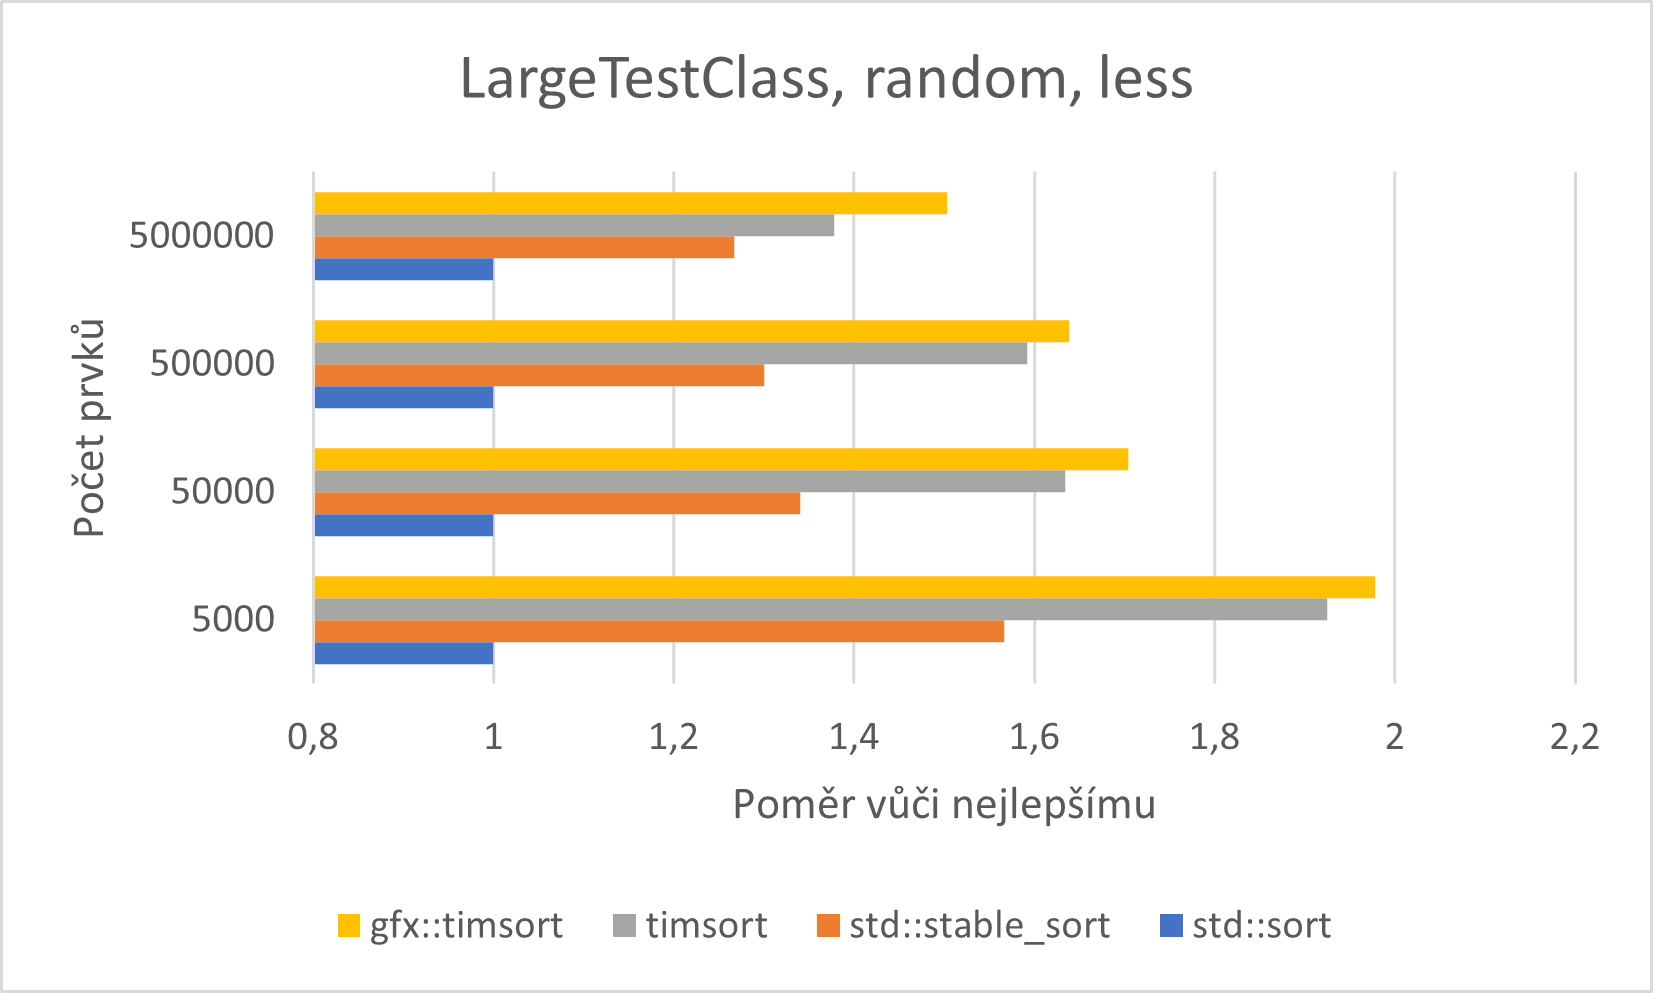
\includegraphics{obrazky/graf1.png}
	\caption[Graf porovnávající náhodná data třídy LargeTestClass pro algoritmy gfx::timsort, timsort, std::stable\_sort a std::sort]{Graf porovnávající náhodná data třídy LargeTestClass pro algoritmy gfx::timsort, timsort, std::stable\_sort a std::sort}\label{fig:graf1}
\end{figure}

\begin{figure}[htbp]\centering
	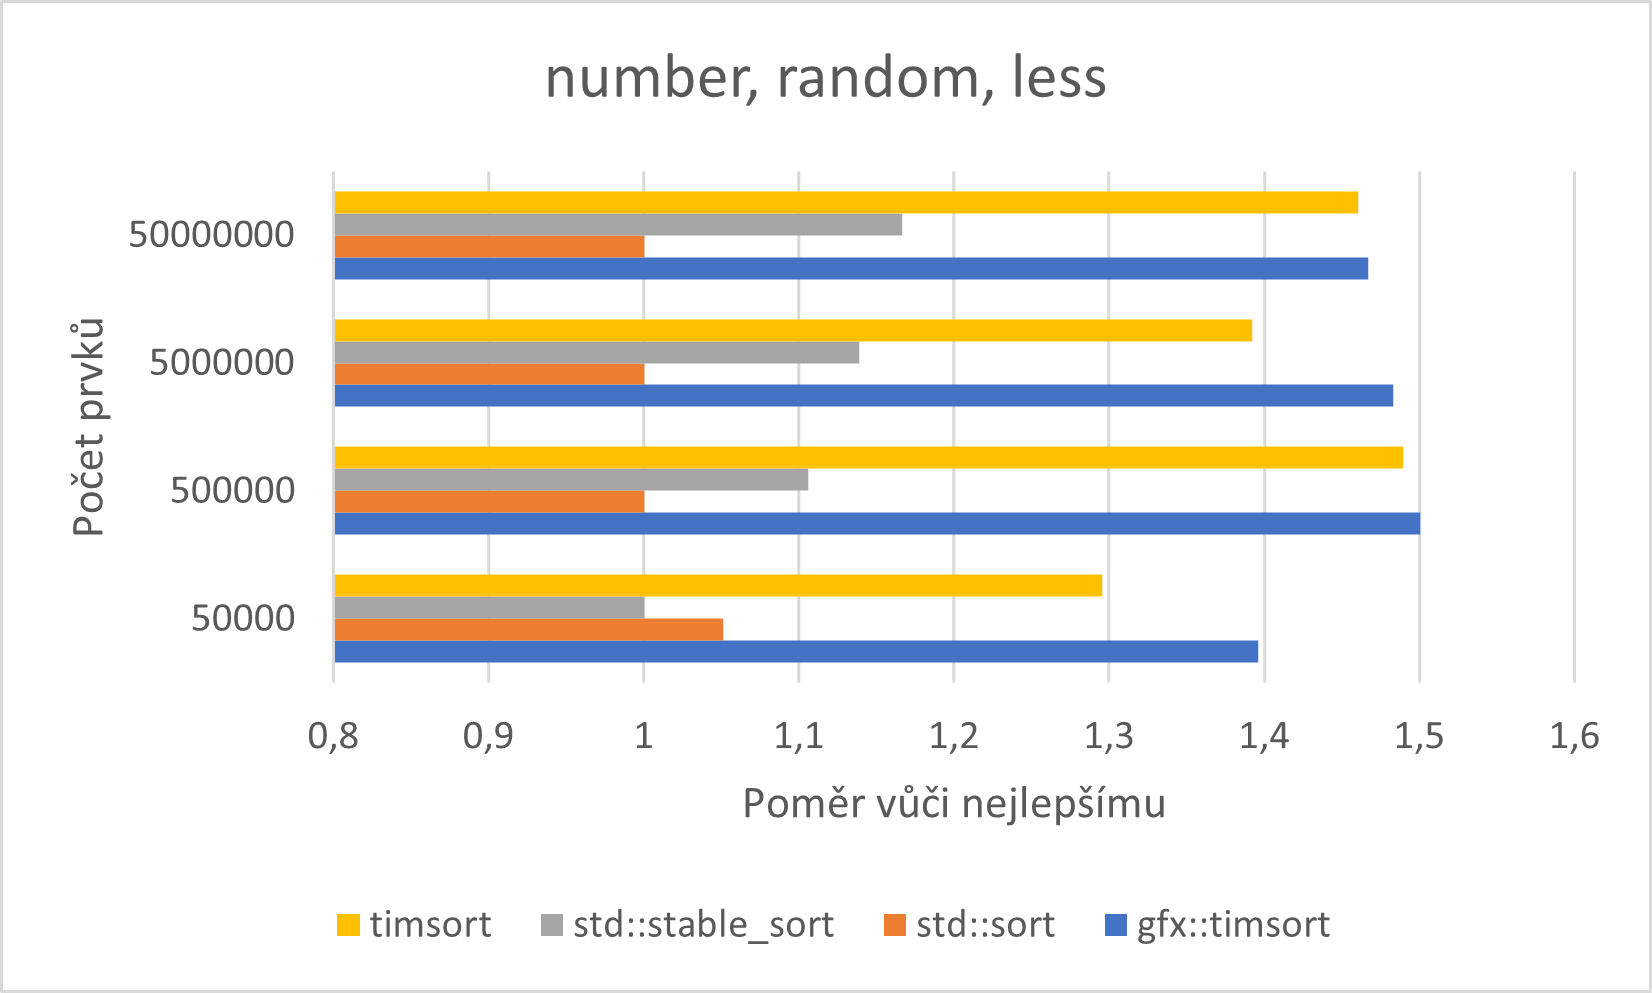
\includegraphics{obrazky/graf2.png}
	\caption[Graf porovnávající náhodná data typu integer pro algoritmy\linebreak gfx::timsort, timsort, std::stable\_sort a std::sort]{Graf porovnávající náhodná data typu integer pro algoritmy gfx::timsort, timsort, std::stable\_sort a std::sort}\label{fig:graf2}
\end{figure}

\begin{figure}[htbp]\centering
	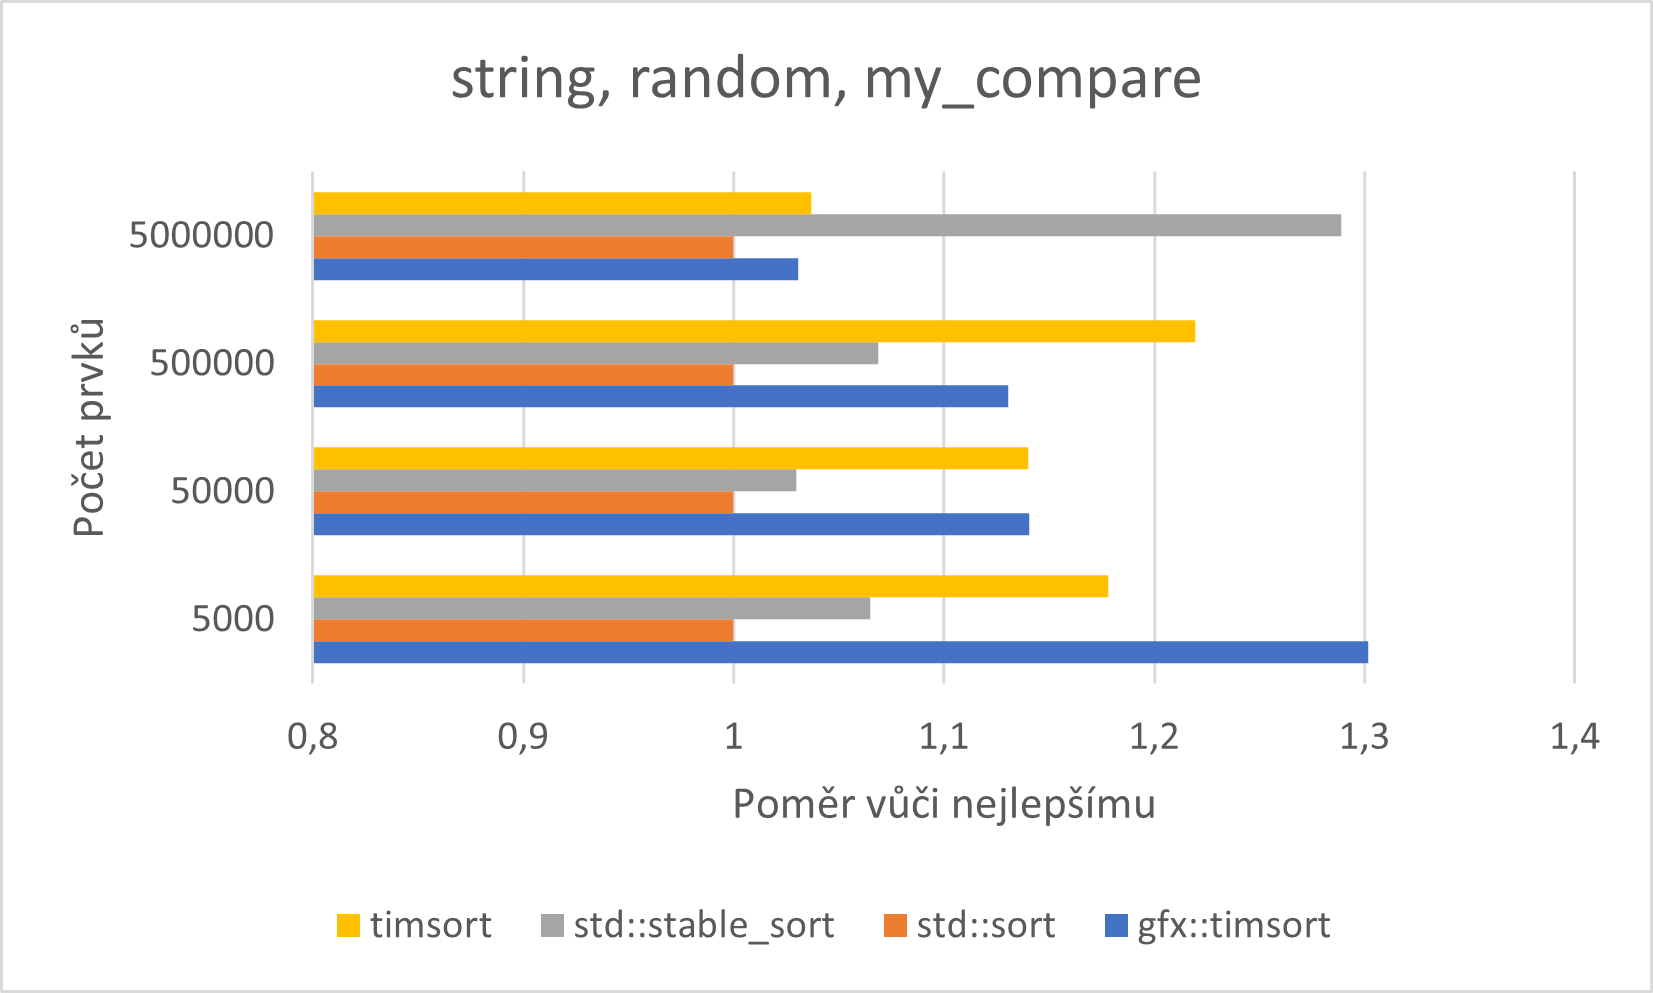
\includegraphics{obrazky/graf3.png}
	\caption[Graf porovnávající náhodná data typu string pro algoritmy\linebreak gfx::timsort, timsort, std::stable\_sort a std::sort]{Graf porovnávající náhodná data typu string pro algoritmy gfx::timsort, timsort, std::stable\_sort a std::sort}\label{fig:graf3}
\end{figure}

\begin{figure}[htbp]\centering
	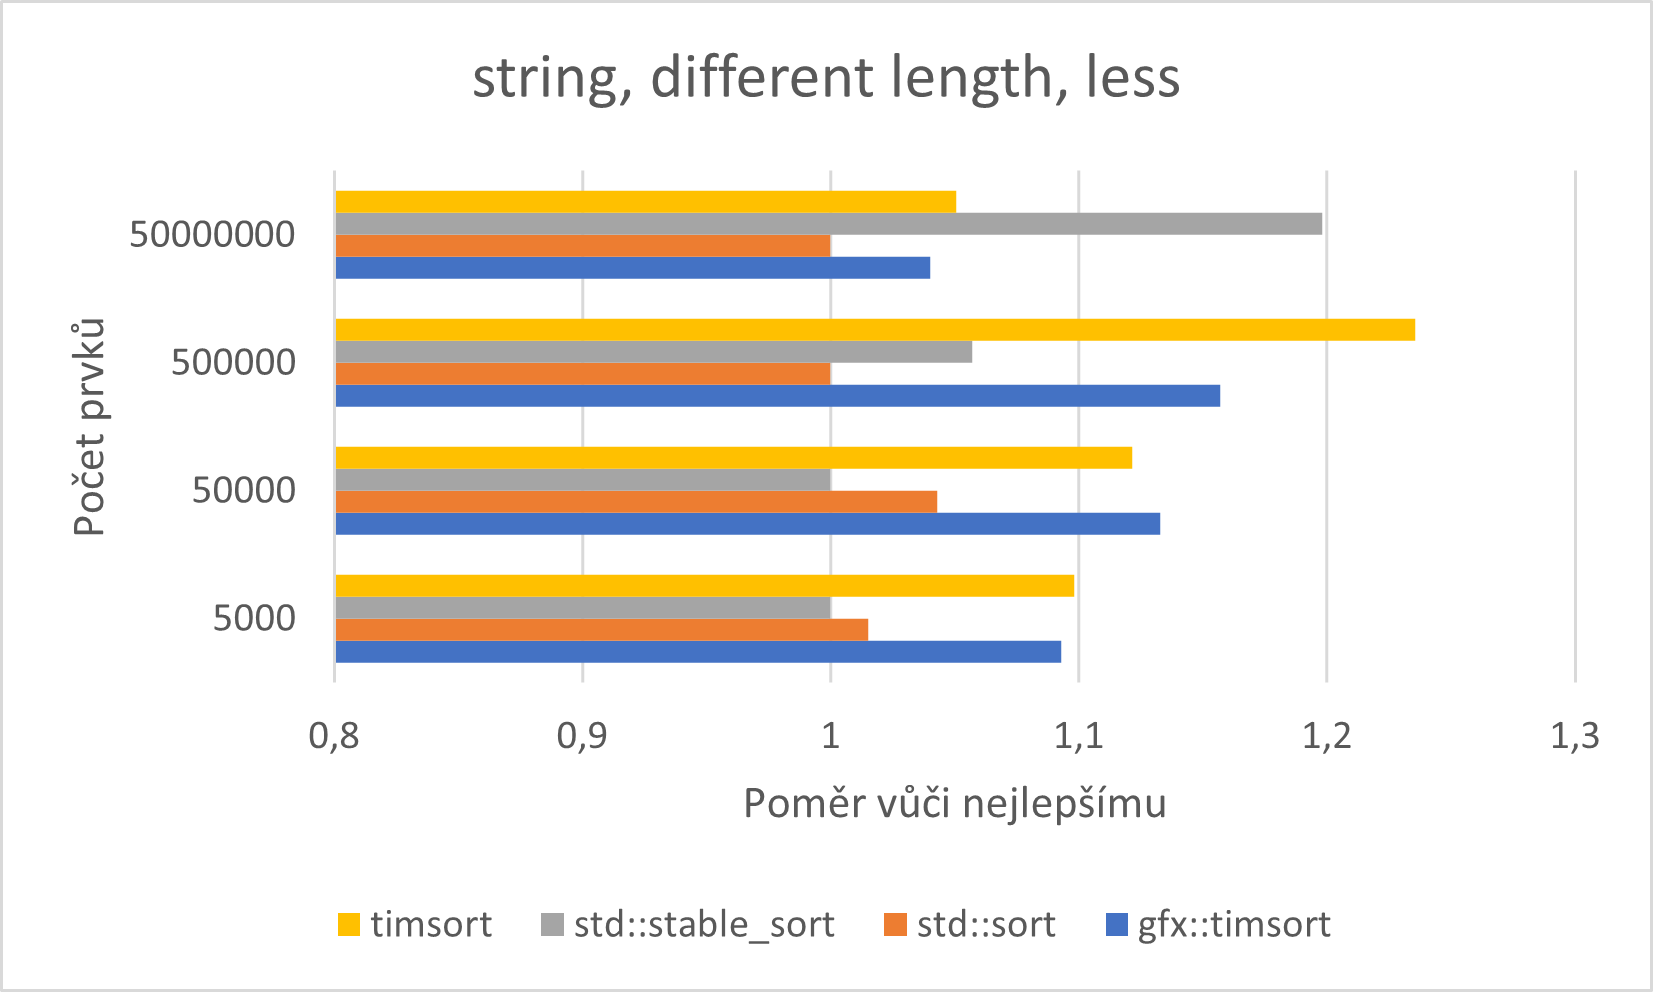
\includegraphics{obrazky/graf4.png}
	\caption[Graf porovnávající náhodná data stringů s různou délkou pro algoritmy gfx::timsort, timsort, std::stable\_sort a std::sort]{Graf porovnávající náhodná data stringů s různou délkou pro algoritmy gfx::timsort, timsort, std::stable\_sort a std::sort}\label{fig:graf4}
\end{figure}

\FloatBarrier

V dalších grafech (\ref{fig:graf5}, \ref{fig:graf6}, \ref{fig:graf7}, \ref{fig:graf8}, \ref{fig:graf9}), kde data obsahují nějaké struktury už můžeme jasně vidět, proč se Timsort využívá přes to, že je pomalejší u náhodných dat. Čím víc jsou data seřazena, tím rychlejší je. Můžeme si také všimnout, že čím víc máme dat, tím víc Timsort vyhrává. Jediná data, která z této části dělají problém, jsou data obsahující mnoho duplikátů. Ovšem i zde je Timsort pouze zhruba 2-krát pomalejší. Porovnáme-li to se seřazenými daty, kde je při 50000000 prvcích zhruba 40-krát rychlejší než \texttt{std::sort} a \texttt{std::stable\_sort} můžeme jasně vidět, proč je tak oblíbený. 

V běžném světě totiž často neřadíme úplně náhodná data, ale například přidáme nějaká data na konec už seřazeného pole. A v tomto případě bude mít Timsort obrovskou výhodu.


\begin{figure}[htbp]\centering
	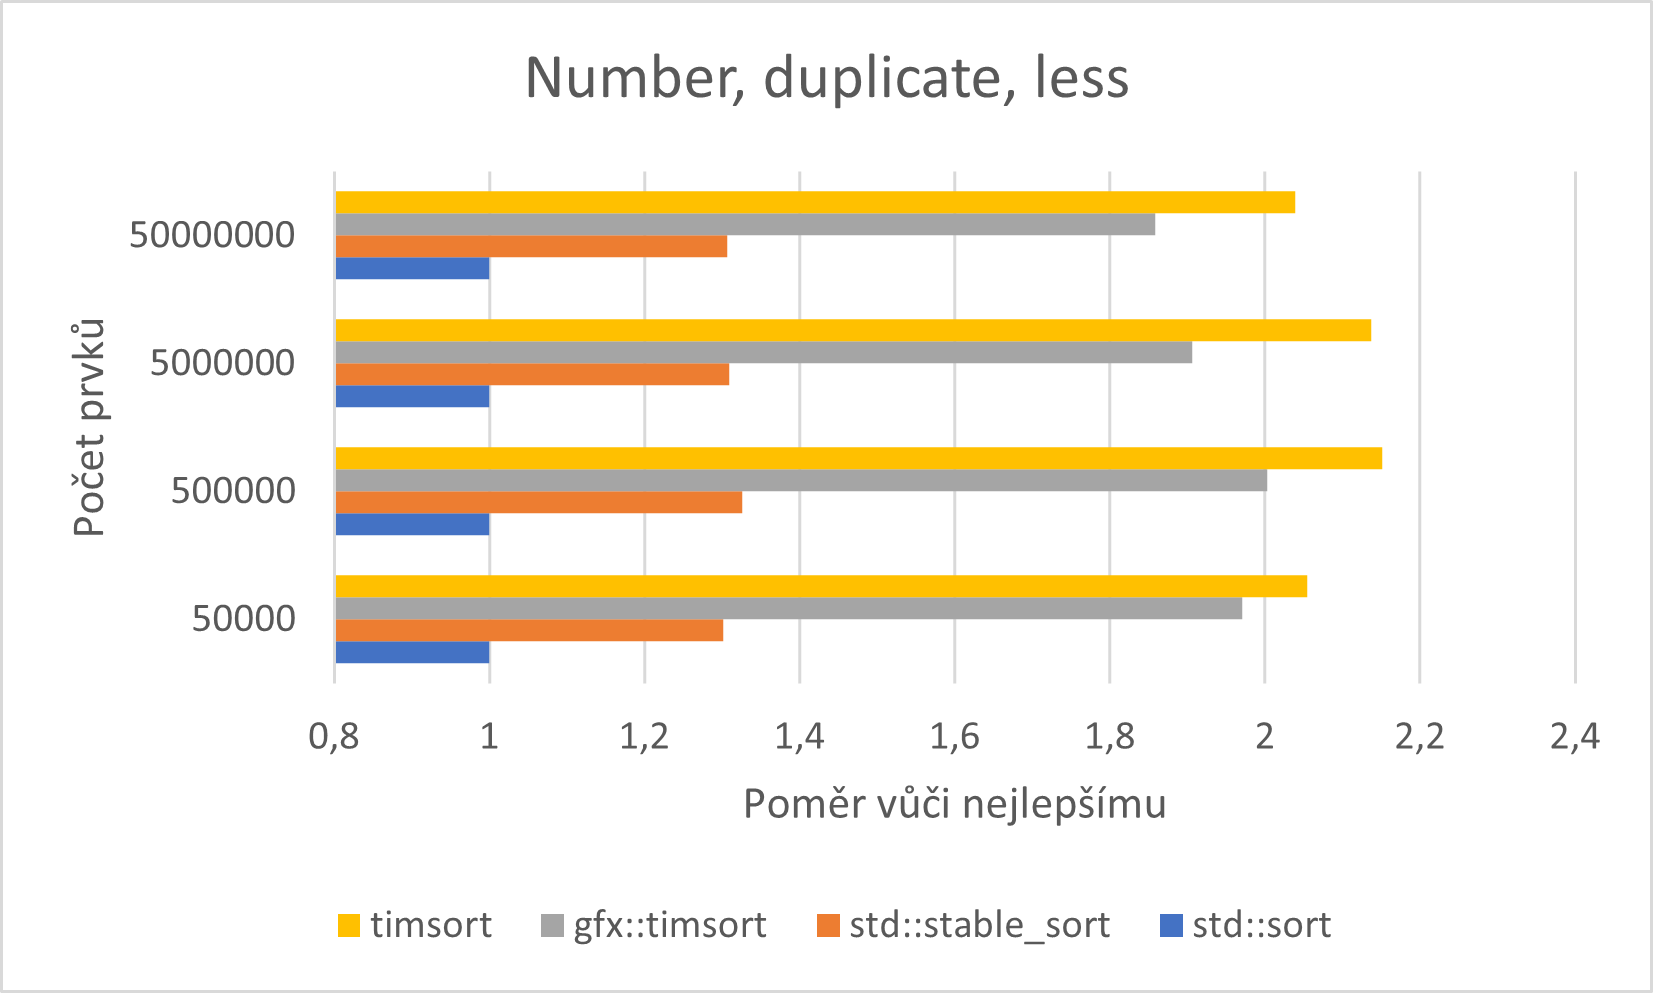
\includegraphics{obrazky/graf5.png}
	\caption[Graf porovnávající data s hodně duplikáty pro algoritmy gfx::timsort, timsort, std::stable\_sort a std::sort]{Graf porovnávající data s hodně duplikáty pro algoritmy gfx::timsort, timsort, std::stable\_sort a std::sort}\label{fig:graf5}
\end{figure}

\begin{figure}[htbp]\centering
	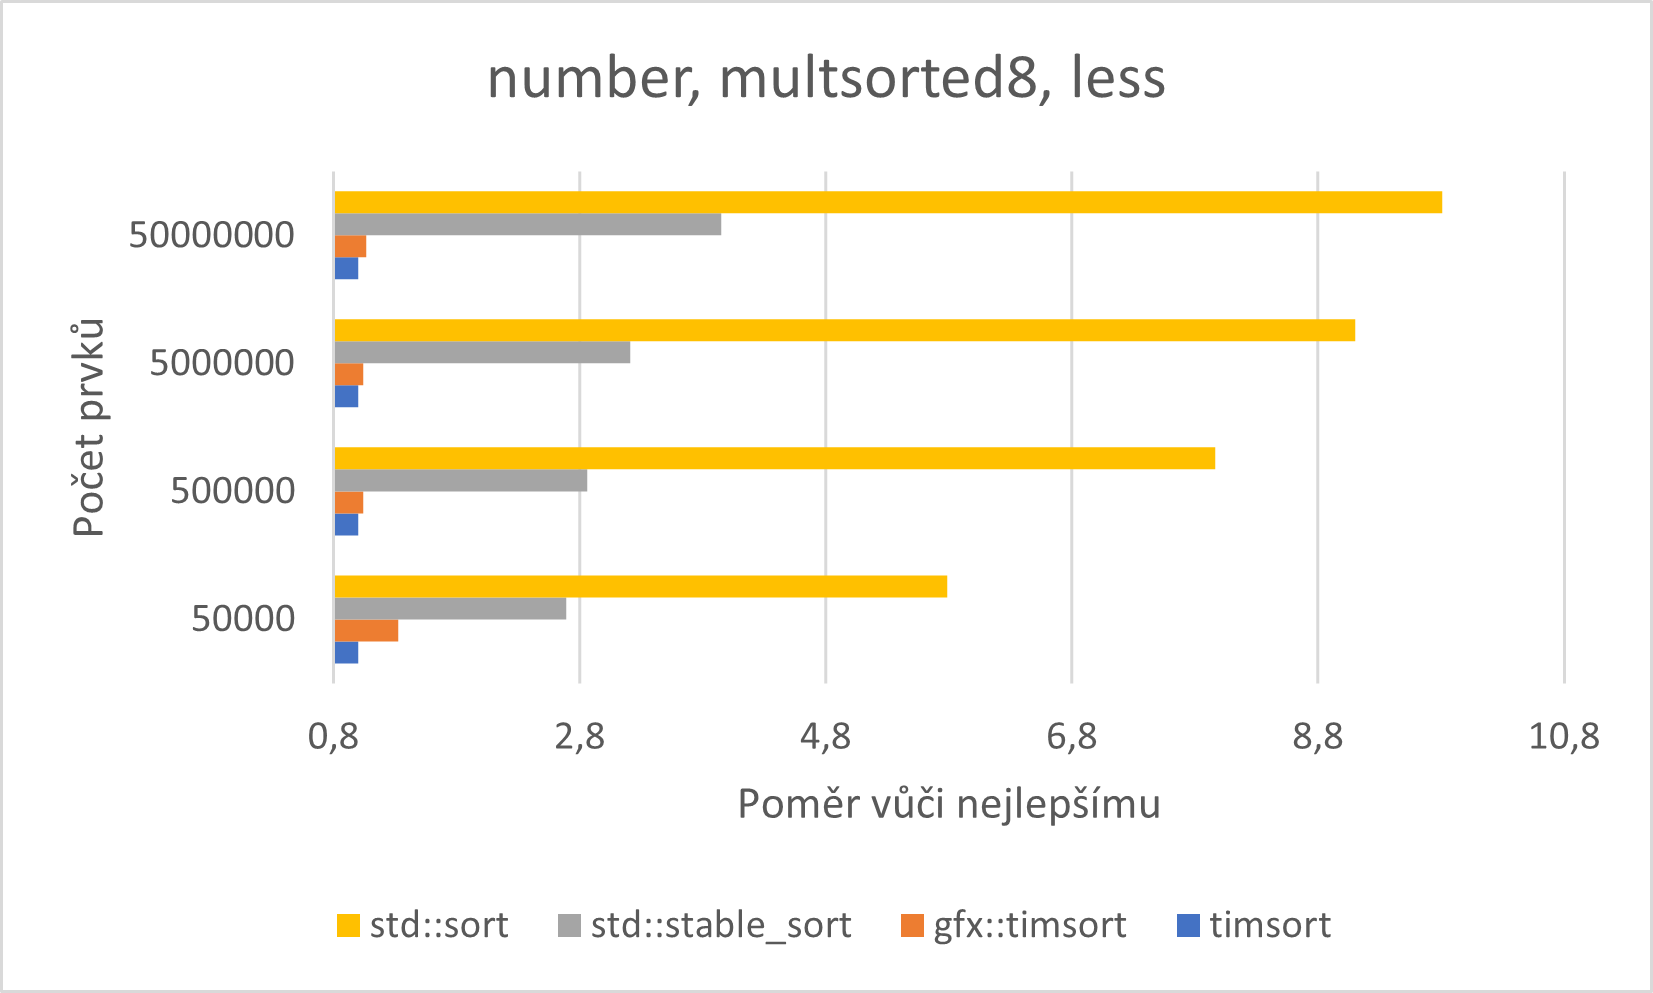
\includegraphics{obrazky/graf6.png}
	\caption[Graf porovnávající data s obsahující několik seřazených částí pro algoritmy gfx::timsort, timsort, std::stable\_sort a std::sort]{Graf porovnávající data s obsahující několik seřazených částí pro algoritmy gfx::timsort, timsort, std::stable\_sort a std::sort}\label{fig:graf6}
\end{figure}

\begin{figure}[htbp]\centering
	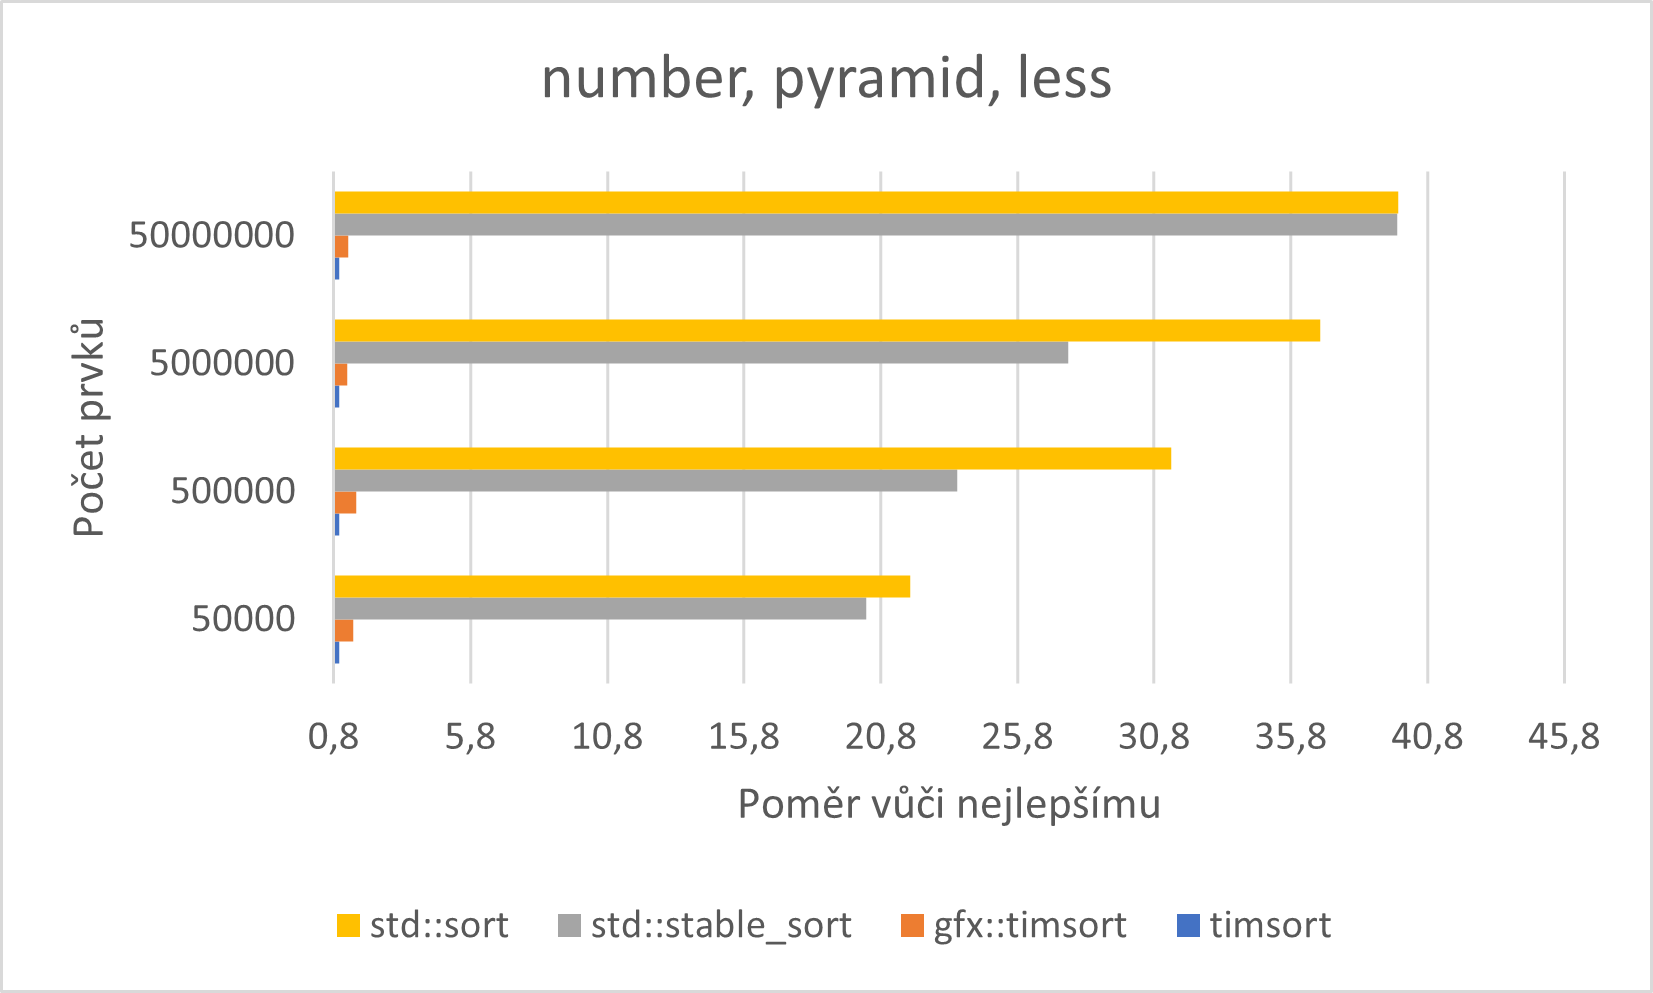
\includegraphics{obrazky/graf7.png}
	\caption[Graf porovnávající data ve tvaru pyramidy pro algoritmy\linebreak gfx::timsort, timsort, std::stable\_sort a std::sort]{Graf porovnávající data ve tvaru pyramidy pro algoritmy gfx::timsort, timsort, std::stable\_sort a std::sort}\label{fig:graf7}
\end{figure}

\begin{figure}[htbp]\centering
	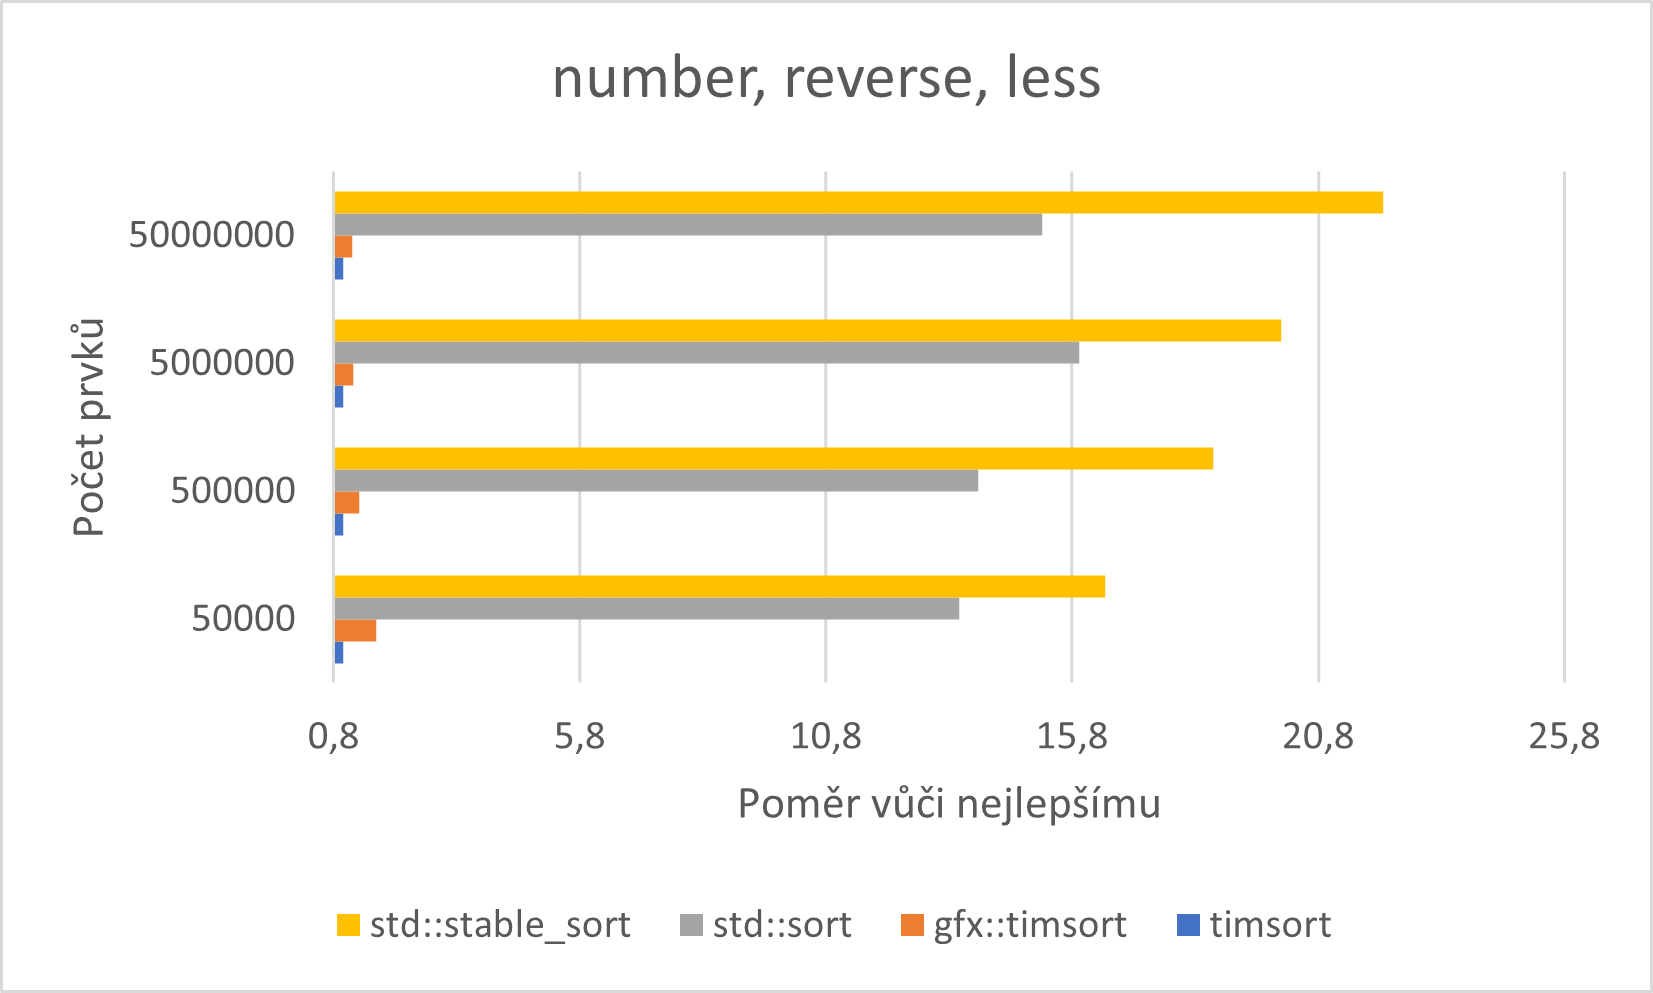
\includegraphics{obrazky/graf8.png}
	\caption[Graf porovnávající data seřazená v opačném pořadí pro algoritmy gfx::timsort, timsort, std::stable\_sort a std::sort]{Graf porovnávající data seřazená v opačném pořadí pro algoritmy gfx::timsort, timsort, std::stable\_sort a std::sort}\label{fig:graf8}
\end{figure}

\begin{figure}[htbp]\centering
	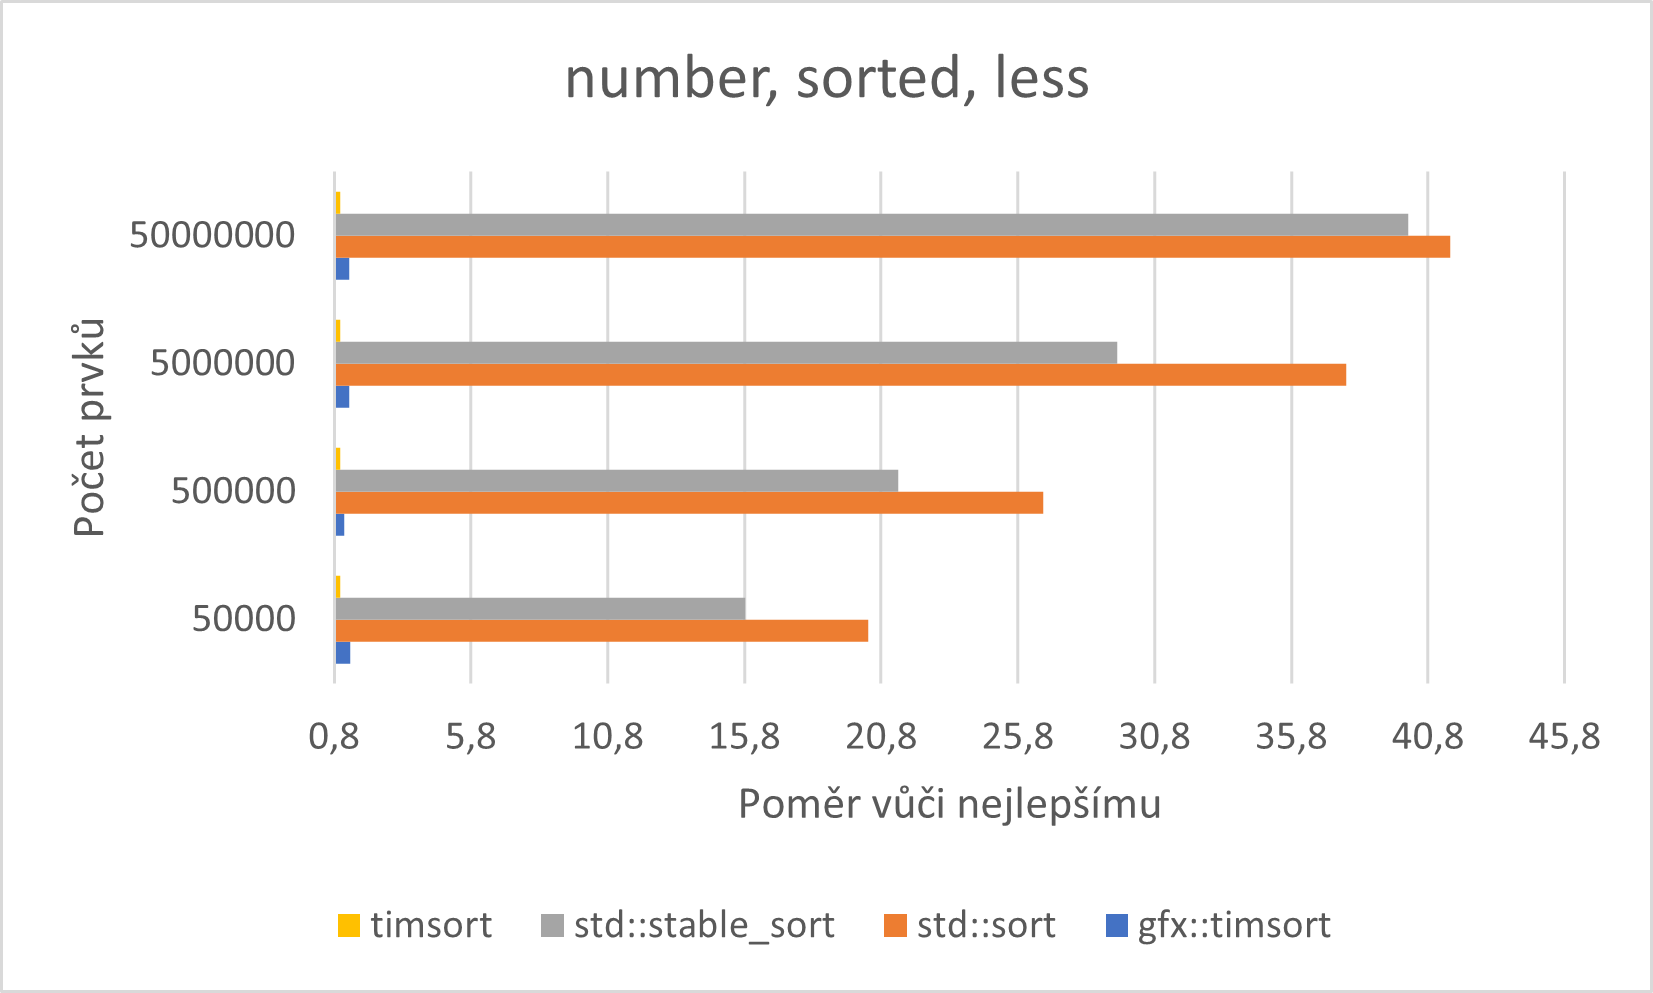
\includegraphics{obrazky/graf9.png}
	\caption[Graf porovnávající seřazená data pro algoritmy gfx::timsort, timsort, std::stable\_sort a std::sort]{Graf porovnávající seřazená data pro algoritmy gfx::timsort, timsort, std::stable\_sort a std::sort}\label{fig:graf9}
\end{figure}


Dalším porovnávacím kritériem, které jsem zvolil je použití různých porovnávacích funkcí. Jak můžeme vidět na následujích grafech (\ref{fig:graf10}, \ref{fig:graf11}, \ref{fig:graf12}), použití jiné funkce může mít poměrně dramatický vliv. Přestože by funkce \texttt{less} a \texttt{my\_compare} měly fungovat stejně, můžeme si všimnout velkého rozdílu. Ten bude pravděpodobně způsoben lepší optimalizací funkce \texttt{less} kompilátorem. Až na výjimku u stringů popsanou v poznámce níže a pár ojedinělých případů, však byla funkce \texttt{less} vždy rychlejší nebo stejně rychlá jako \texttt{my\_compare}. Jeden z těchto případů je popsán v sekci Testování optimalizací v tabulce \ref{tab:tab4}.

\begin{figure}[htbp]\centering
	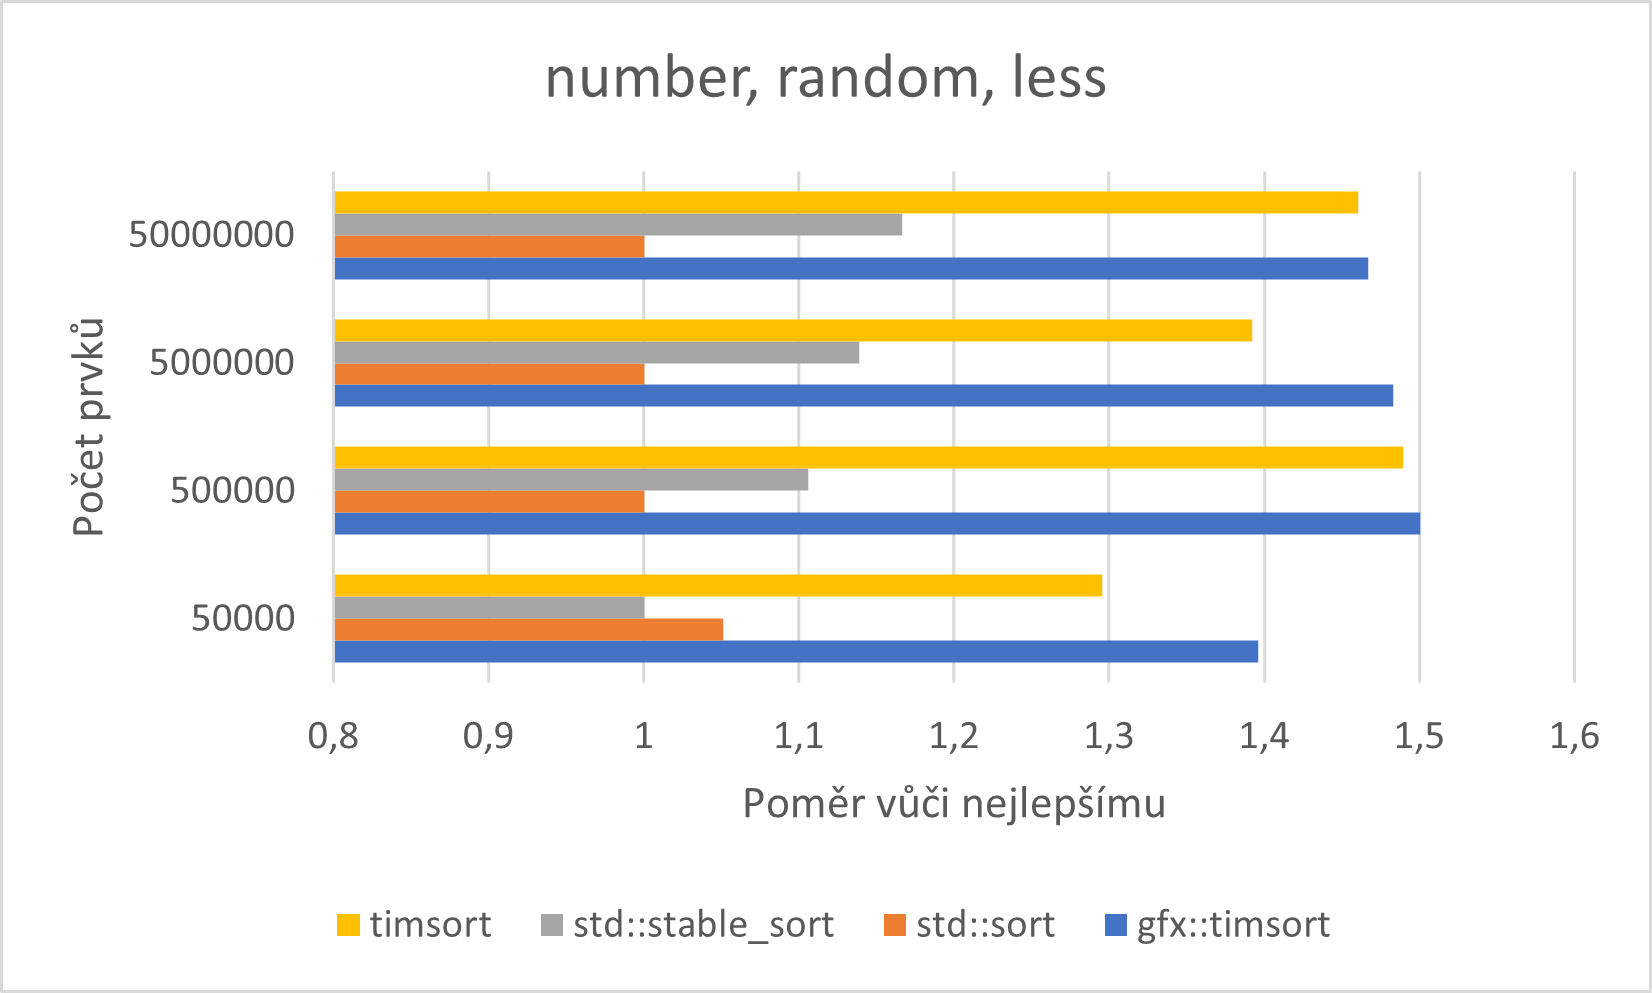
\includegraphics{obrazky/graf10.png}
	\caption[Graf porovnávající náhodná data řazena funkcí less pro algoritmy gfx::timsort, timsort, std::stable\_sort a std::sort]{Graf porovnávající náhodná data řazena funkcí less pro algoritmy gfx::timsort, timsort, std::stable\_sort a std::sort}\label{fig:graf10}
\end{figure}

\begin{figure}[htbp]\centering
	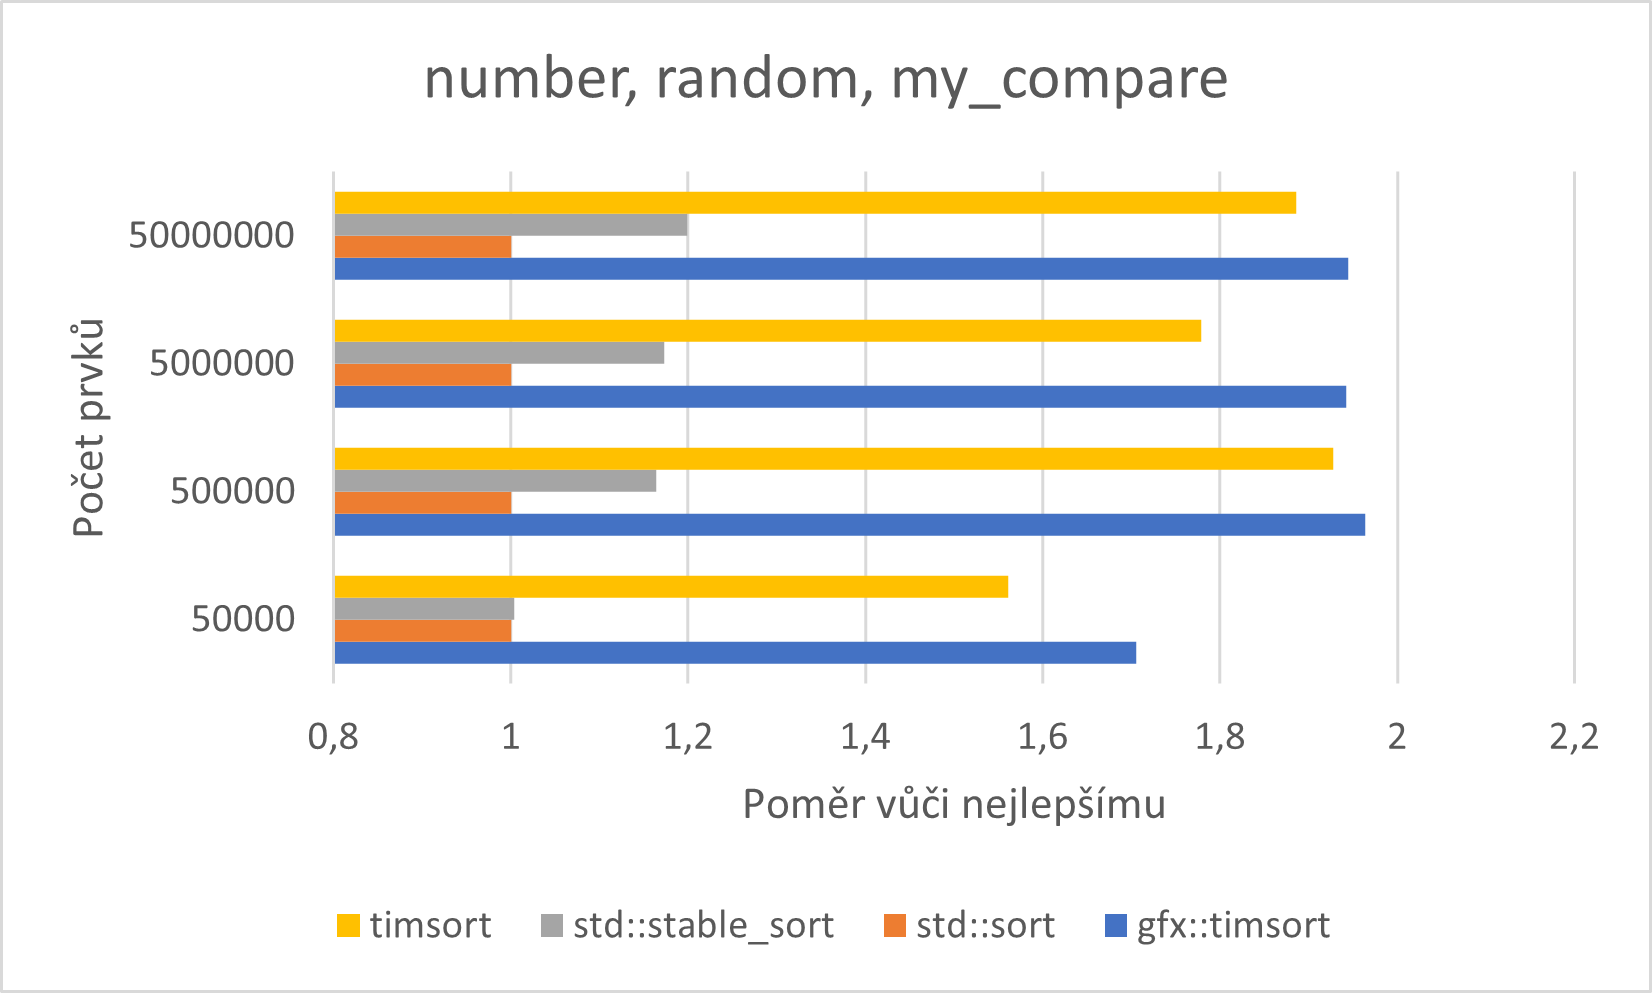
\includegraphics{obrazky/graf11.png}
	\caption[Graf porovnávající náhodná data řazena funkcí my\_compare pro algoritmy gfx::timsort, timsort, std::stable\_sort a std::sort]{Graf porovnávající náhodná data řazena funkcí my\_compare pro algoritmy gfx::timsort, timsort, std::stable\_sort a std::sort}\label{fig:graf11}
\end{figure}

\begin{figure}[htbp]\centering
	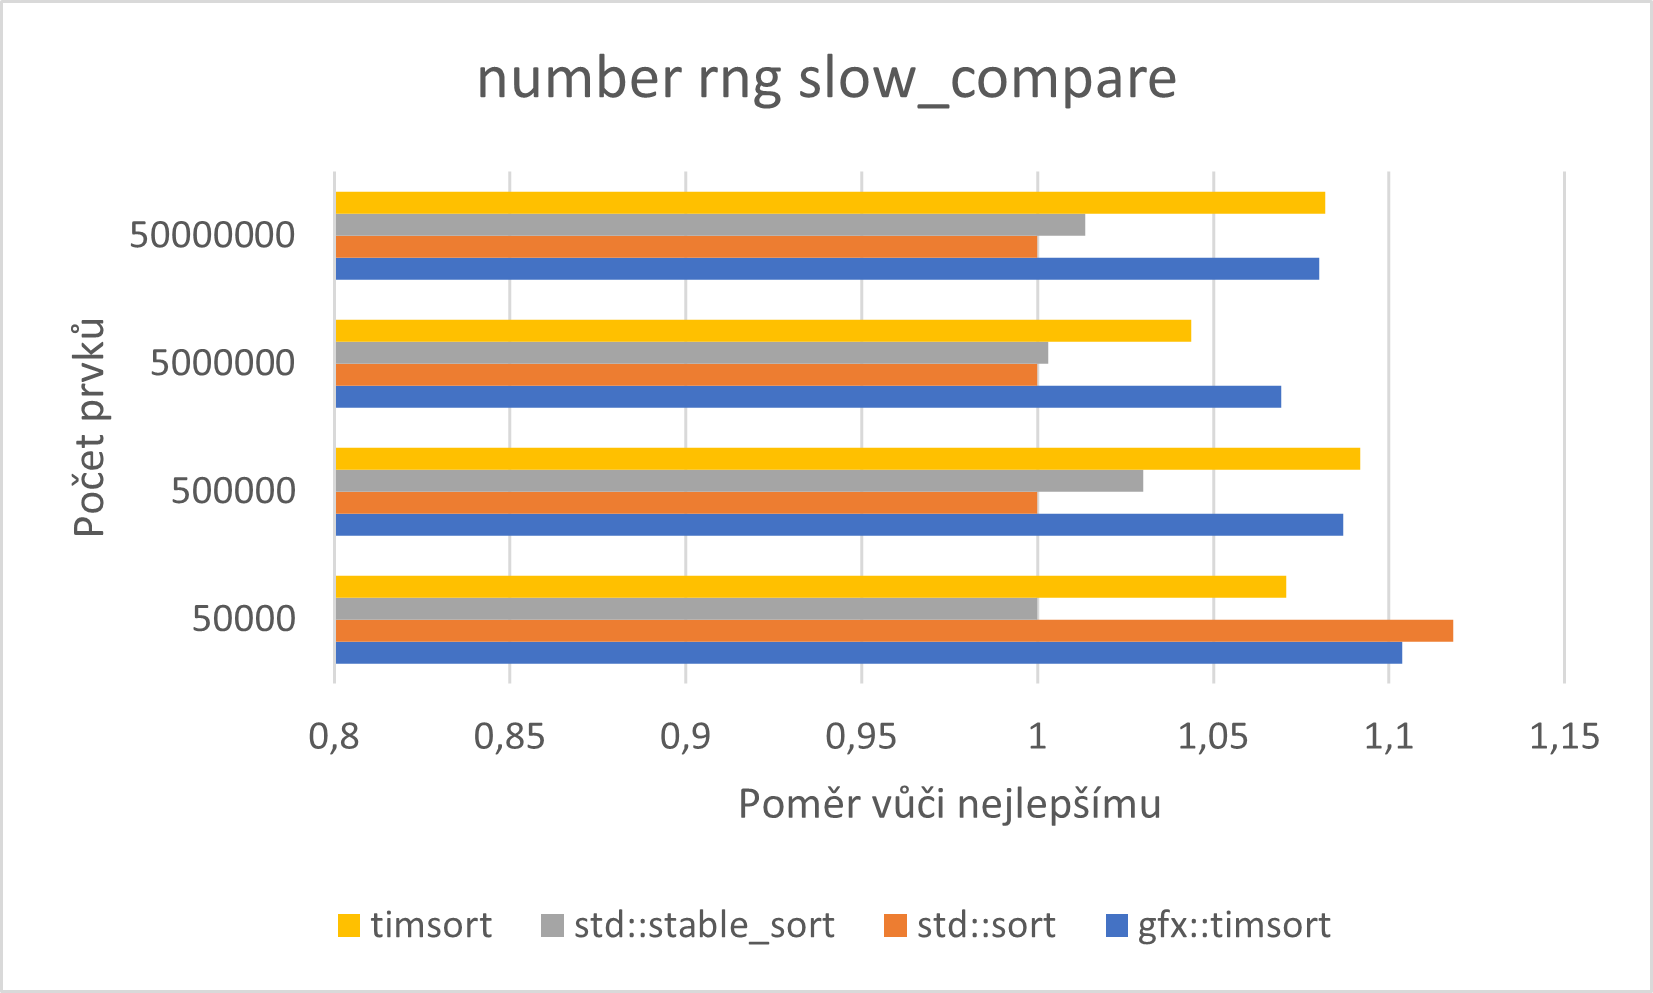
\includegraphics{obrazky/graf12.png}
	\caption[Graf porovnávající náhodná data řazena funkcí slow\_compare pro algoritmy gfx::timsort, timsort, std::stable\_sort a std::sort]{Graf porovnávající náhodná data řazena funkcí slow\_compare pro algoritmy gfx::timsort, timsort, std::stable\_sort a std::sort}\label{fig:graf12}
\end{figure}

\begin{figure}[htbp]\centering
	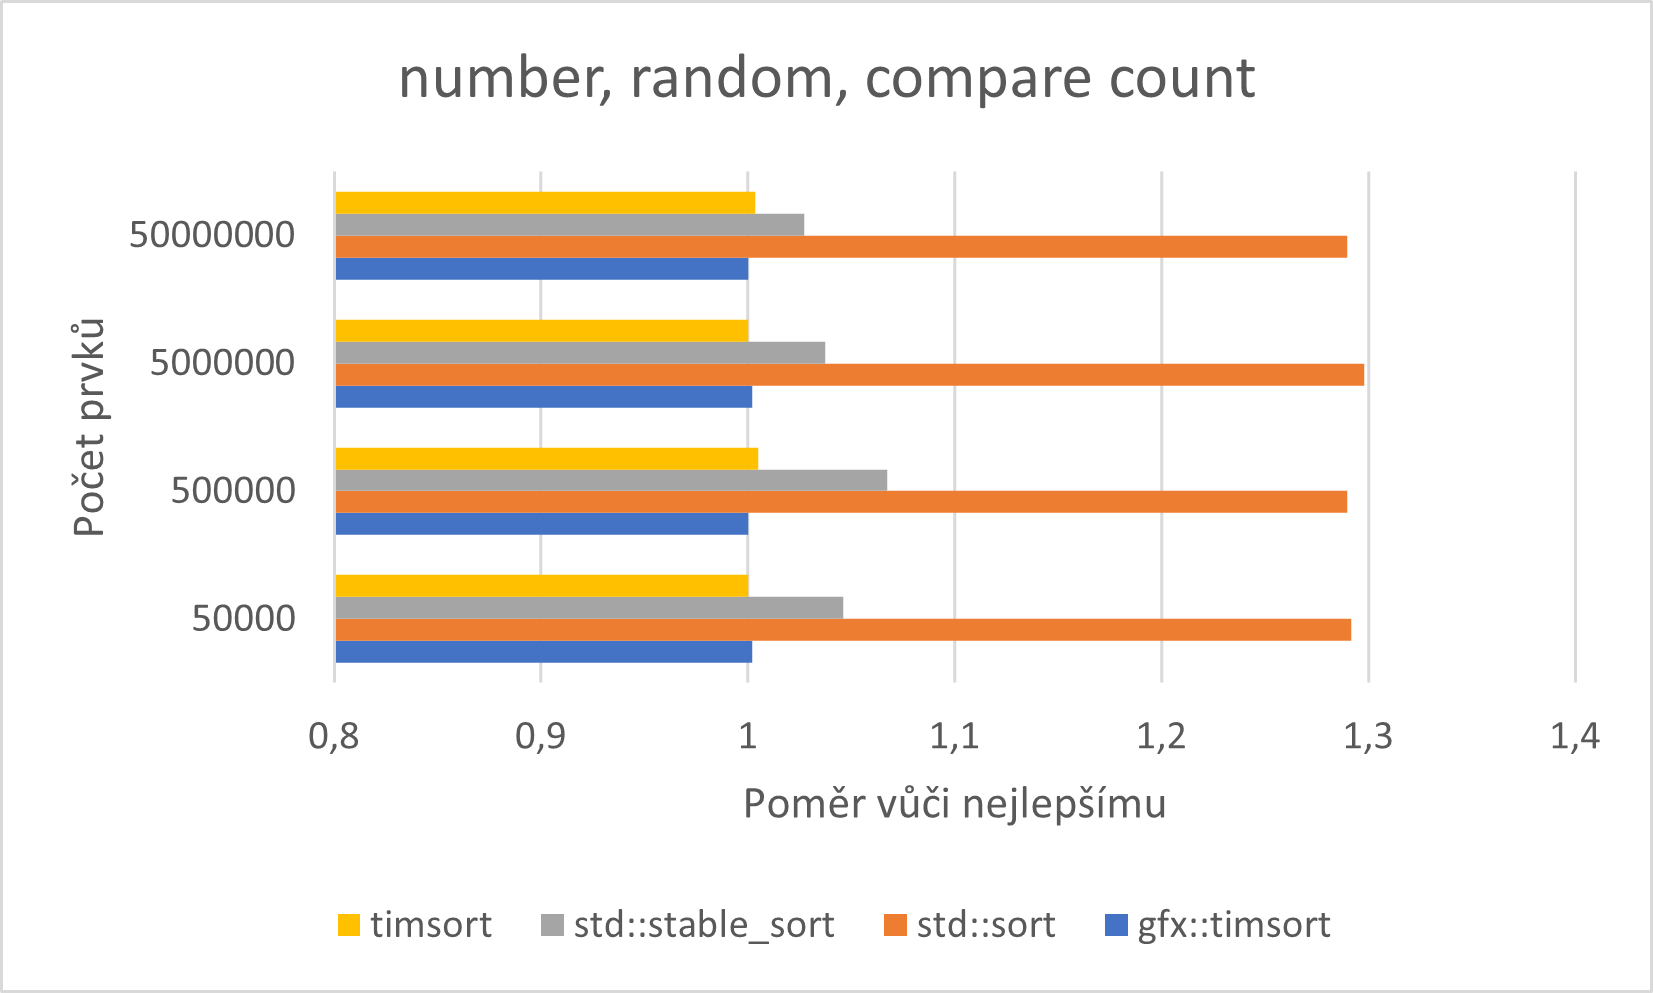
\includegraphics{obrazky/graf13.png}
	\caption[Graf zobrazující počet porovnání náhodných dat pro algoritmy gfx::timsort, timsort, std::stable\_sort a std::sort]{Graf zobrazující počet porovnání náhodných dat pro algoritmy gfx::timsort, timsort, std::stable\_sort a std::sort}\label{fig:graf13}
\end{figure}


Na posledním grafu (\ref{fig:graf13}) je také zobrazen relativní počet potřebných porovnání řadících algoritmů. Můžeme vidět, že Timsorty vyžadují nejméně porovnání. To vysvětluje proč jsou s řadící funkcí \texttt{slow\_compare} Timsorty skoro stejně rychlé jako nejrychlejší \texttt{std::sort}. Kdyby byla porovnávací funkce ještě o něco pomalejší, tak by Timsorty začaly být rychlejší. To je také ten důvod, proč se Timsort používá především pro neprimitivní typy, které mohou mít složité porovnávání.

\FloatBarrier


\subsection{Shrnutí testování základní verze Timsortu}

V této sekci jsme porovnávali mou implementaci Timsortu. Ta obstála v porovnáním s Timsortem z knihovny \texttt{gfx} a chovala se přesně tak, jak bychom od Timsortu očekávali. Zajímavostí je, že se obě implementace drobně liší a v závislosti na datech mezi nimi jsou drobné rozdíly v rychlosti. 

Dále máme porovnání s dalšími řadícími algoritmy a to konkrétně\linebreak \texttt{std::sort} založený na Introsortu a \texttt{std::stable\_sort} založený na Mergesortu. Můžeme si všimnout, že ačkoliv jsou tyto algoritmy rychlejší pro náhodná data, tak data obsahující struktury jim v porovnání s Timsortem dělají problém.

Výsledné porovnání algoritmů pro 50000000 integerů s různými strukturami (\ref{fig:graf14}). Vzhledem k logaritmickému měřítku doby běhu nemusí být na první pohled jasné obrovské zrychlení pro různě seřazená pole. Ještě jednou si můžeme na tomto grafu povšimnout, že se oba Timsorty opravdu chovají identicky.

\begin{figure}[htbp]\centering
	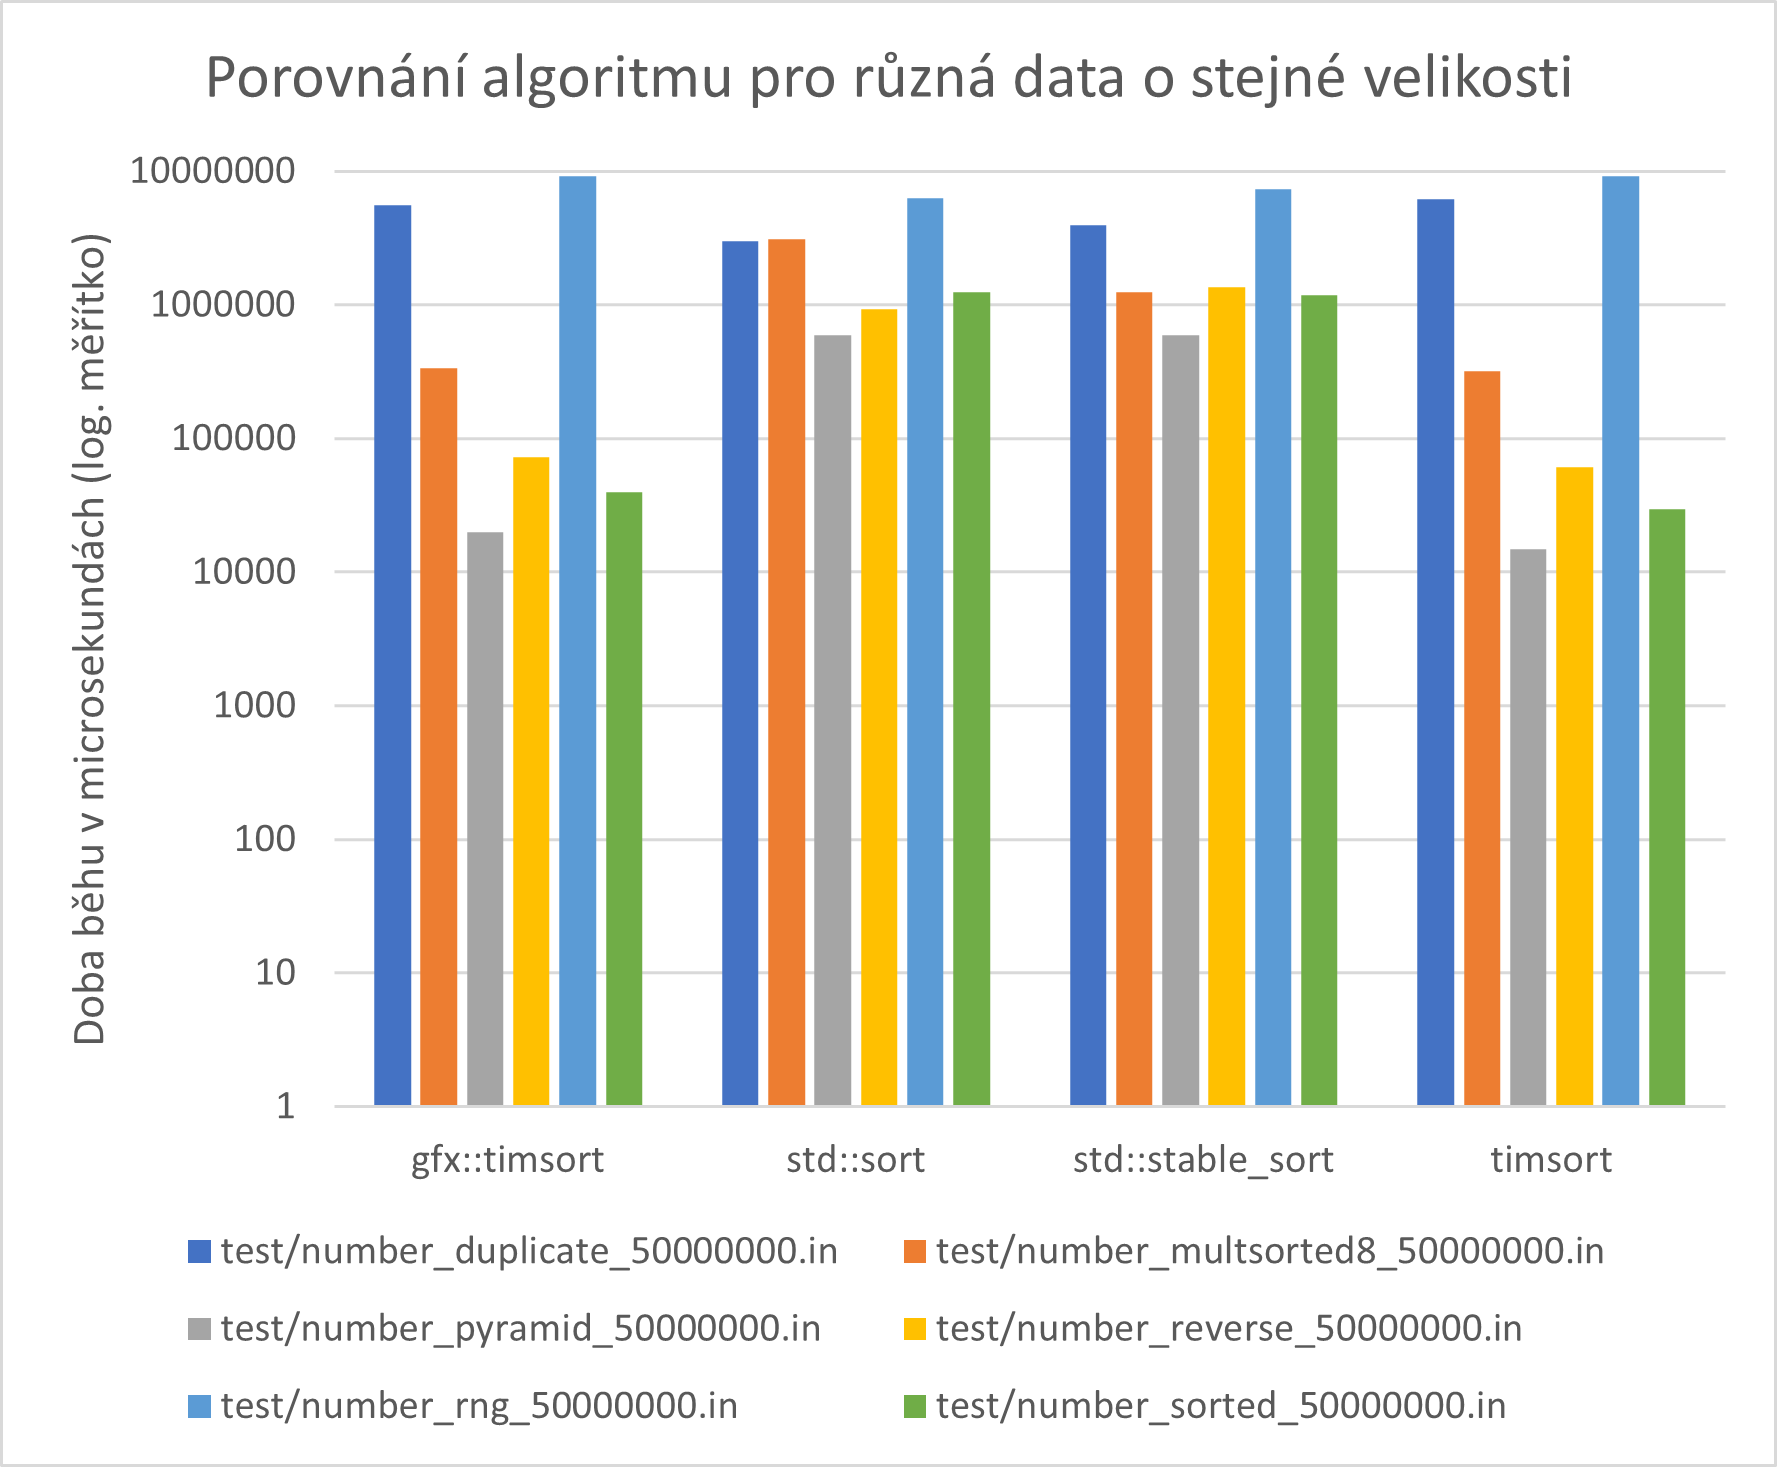
\includegraphics[width=13cm]{obrazky/graf14.png}
	\caption[Graf porovnávající algoritmy gfx::timsort, std::sort, std::stable\_sort a timsort na různých datech o stejné velikosti]{Graf porovnávající algoritmy gfx::timsort, std::sort, std::stable\_sort a timsort na různých datech o stejné velikosti}\label{fig:graf14}
\end{figure}

\subsection{Poznámka k testování stringů}
Během testování stringů se objevil problém s porovnávací funkcí \texttt{less} a některými algoritmy (tabulka \ref{tab:tab2}). Zatímco algoritmus \texttt{std::sort} vracel očekávané hodnoty vždy, tak pro ostatní algoritmy byl problém s menším počtem prvků. Ve výsledku to vypadalo tak, že pro 5000 prvků byl algoritmus výrazně pomalejší. Dokonce byl pomalejší než ten samý algoritmus, také s porovnávací funkcí \texttt{less} pro 50000 prvků. Proto prezentuji výsledky funkce \texttt{my\_compare}, kde už všechny hodnoty odpovídají očekávání.

\begin{table}[htbp]\centering
	\caption[Porovnání funkce less a my\_compare u stringů]{Porovnání funkce less a my\_compare u stringů}\label{tab:tab2}
	\begin{tabular}{|c|c|c|c|}\hline
		Počet prvků		& algoritmus		& less	& my\_compare	\tabularnewline \hline \hline
 		5000		& gfx::timsort		& 17492	& 1584		\tabularnewline \hline
 		5000		& std::sort		& 1307	& 1217		\tabularnewline \hline
 		5000		& std::stable\_sort		& 15585	& 1296		\tabularnewline \hline
 		5000		& timsort		& 15642	& 1434		\tabularnewline \hline
  		50000		& gfx::timsort		& 19712	& 19839		\tabularnewline \hline
 		50000		& std::sort		& 16746	& 17396		\tabularnewline \hline
 		50000		& std::stable\_sort		& 16229	& 17917		\tabularnewline \hline
 		50000		& timsort		& 18521	& 19833		\tabularnewline \hline
  		500000		& gfx::timsort		& 247781	& 260819		\tabularnewline \hline
 		500000		& std::sort		& 220812	& 230737		\tabularnewline \hline
 		500000		& std::stable\_sort		& 219269	& 246606		\tabularnewline \hline
 		500000		& timsort		& 262599	& 281412		\tabularnewline \hline
 		5000000		& gfx::timsort		& 3482919	& 3658339		\tabularnewline \hline
 		5000000		& std::sort		& 3435478	& 3549239		\tabularnewline \hline
 		5000000		& std::stable\_sort		& 4039618	& 4574116		\tabularnewline \hline
 		5000000		& timsort		& 3434988	& 3680149		\tabularnewline \hline
 	\end{tabular}
\end{table}

\section{Testování optimalizací}

\subsection{Hledání runu od konce}

Tohoto porovnání se zúčastní 4 algoritmy -- \texttt{timsort}, \texttt{timsort\_rev},\linebreak \texttt{it\_merge\_2\_sort} a \texttt{it\_merge\_2\_sort\_rev}. Při prozkoumaní grafů níže (\ref{fig:graf15}, \ref{fig:graf16}) zjistíme, že "reverzní" algoritmy opravdu občas vyhrají -- přesně tak jak bylo napsáno v komentáři u implementace řadící algoritmu v Rustu. Při podrobnějším zkoumání však zjistíme, že se nedá říci, který algoritmus je lepší. V jednom testu vyjdou nejlépe reverzní verze a v jiném zase normální verze. Při některých testech se dokonce stalo, že jedna reverzní verze byla nejrychlejší a druhá nejpomalejší. Proto jsou zde pouze dva grafy na ukázku, že se reverzní algoritmy s normálními střídají. Ačkoliv zrychlení mohlo dosáhnout i 20\% bude pravděpodobně záležet na konkrétních datech. Abychom toto vyvrátili, bylo by potřeba testy opakovat s obrovským množstvím různých dat. Mým odhadem je, že to záleží na využívání dat v cache paměti a v některých případech používáme častěji ty samá data. Tím bychom tedy získali zrychlení. Bohužel se v takovém případě nedá mluvit o žádné struktuře dat, kterou bychom mohli předem znát. 


\begin{figure}[htbp]\centering
	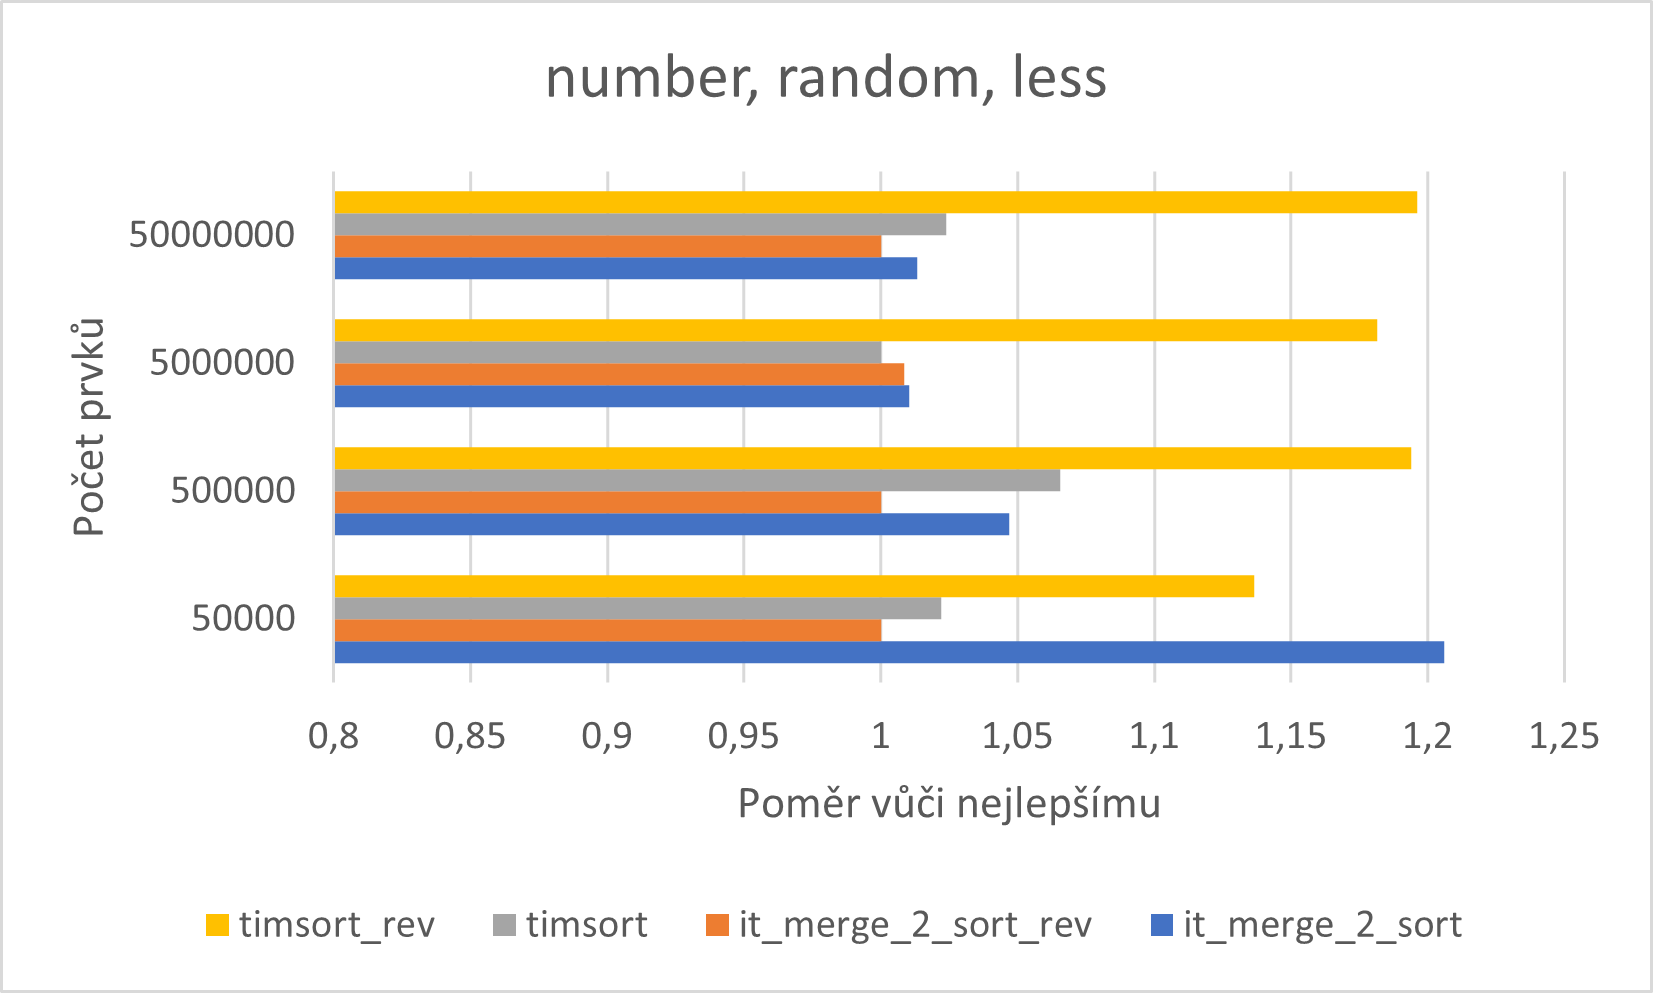
\includegraphics{obrazky/graf15.png}
	\caption[Graf porovnávající algoritmy timsort\_rev, timsort,\linebreak it\_merge\_2\_sort\_rev a it\_merge\_2\_sort na náhodných datech]{Graf porovnávající algoritmy timsort\_rev, timsort, it\_merge\_2\_sort\_rev a it\_merge\_2\_sort na náhodných datech}\label{fig:graf15}
\end{figure}

\begin{figure}[htbp]\centering
	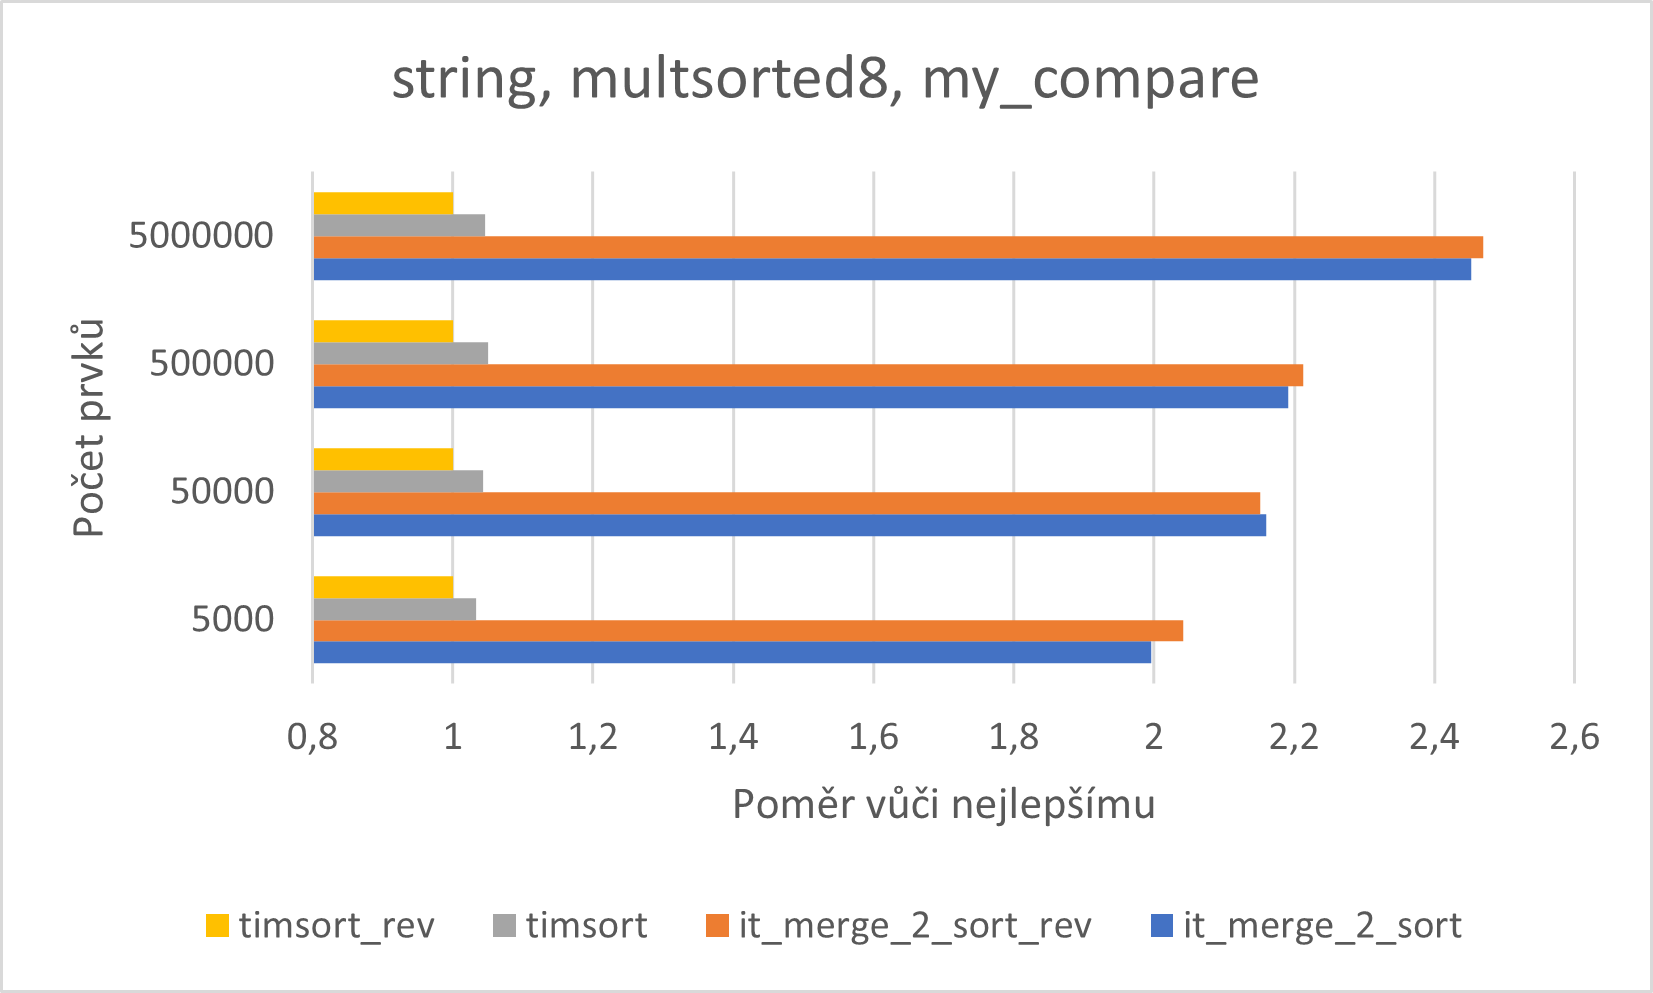
\includegraphics{obrazky/graf16.png}
	\caption[Graf porovnávající algoritmy timsort\_rev, timsort,\linebreak it\_merge\_2\_sort\_rev a it\_merge\_2\_sort na několika seřazených částech]{Graf porovnávající algoritmy timsort\_rev, timsort, it\_merge\_2\_sort\_rev a it\_merge\_2\_sort na několika seřazených částech}\label{fig:graf16}
\end{figure}

\subsection{Mergování více runů}

Tohoto porovnání se účastnili algoritmy \texttt{it\_merge\_2\_sort}, \texttt{it\_merge\_3\_sort}, \texttt{it\_merge\_4a\_sort} a \texttt{it\_merge\_4b\_sort} a jejich rekurzivní verze. Rekurzivní verze ovšem vynechám ve výsledcích zde, protože bychom přišli o adaptivitu Timsortu, pokud bychom je využili. Platilo pravidlo, že rekurzivní algoritmy byly ve stejném pořadí jako iterativní a byly oproti iterativním o něco málo rychlejší. Z grafů \ref{fig:graf17}, \ref{fig:graf18} a \ref{fig:graf19} lze vyvodit následující:

Algoritmus \texttt{it\_merge\_4a\_sort} a algoritmus \texttt{it\_merge\_2\_sort} dopadly většinou podobně. Rozdíl byl pokud jsme řadili větší objekt. Pak byl rychlejší algoritmus \texttt{it\_merge\_4a\_sort}, tak jak bychom očekávali, díky ušetřenému kopírování.

Algoritmus \texttt{it\_merge\_4b\_sort} byl nejrychlejší pokud byla porovnávací funkce rychlá. Jakmile však byla porovnávací funkce pomalá, byl nejpomalejší. Zpomalení způsobeno tím, že oproti ostatním zmíněným algoritmům potřebuje mnohem více porovnání.

Poslední algoritmus \texttt{it\_merge\_3\_sort} byl ze zmíněných asi nejvíce všestranný. Využil zrychlení stejně jako v případě \texttt{it\_merge\_4b\_sortu}, ale nepotřebuje tolik porovnání (tabulka \ref{tab:tab3}). Přesto jich potřebuje více než\linebreak \texttt{it\_merge\_4a\_sort} a \texttt{it\_merge\_2\_sort}. 


\begin{figure}[htbp]\centering
	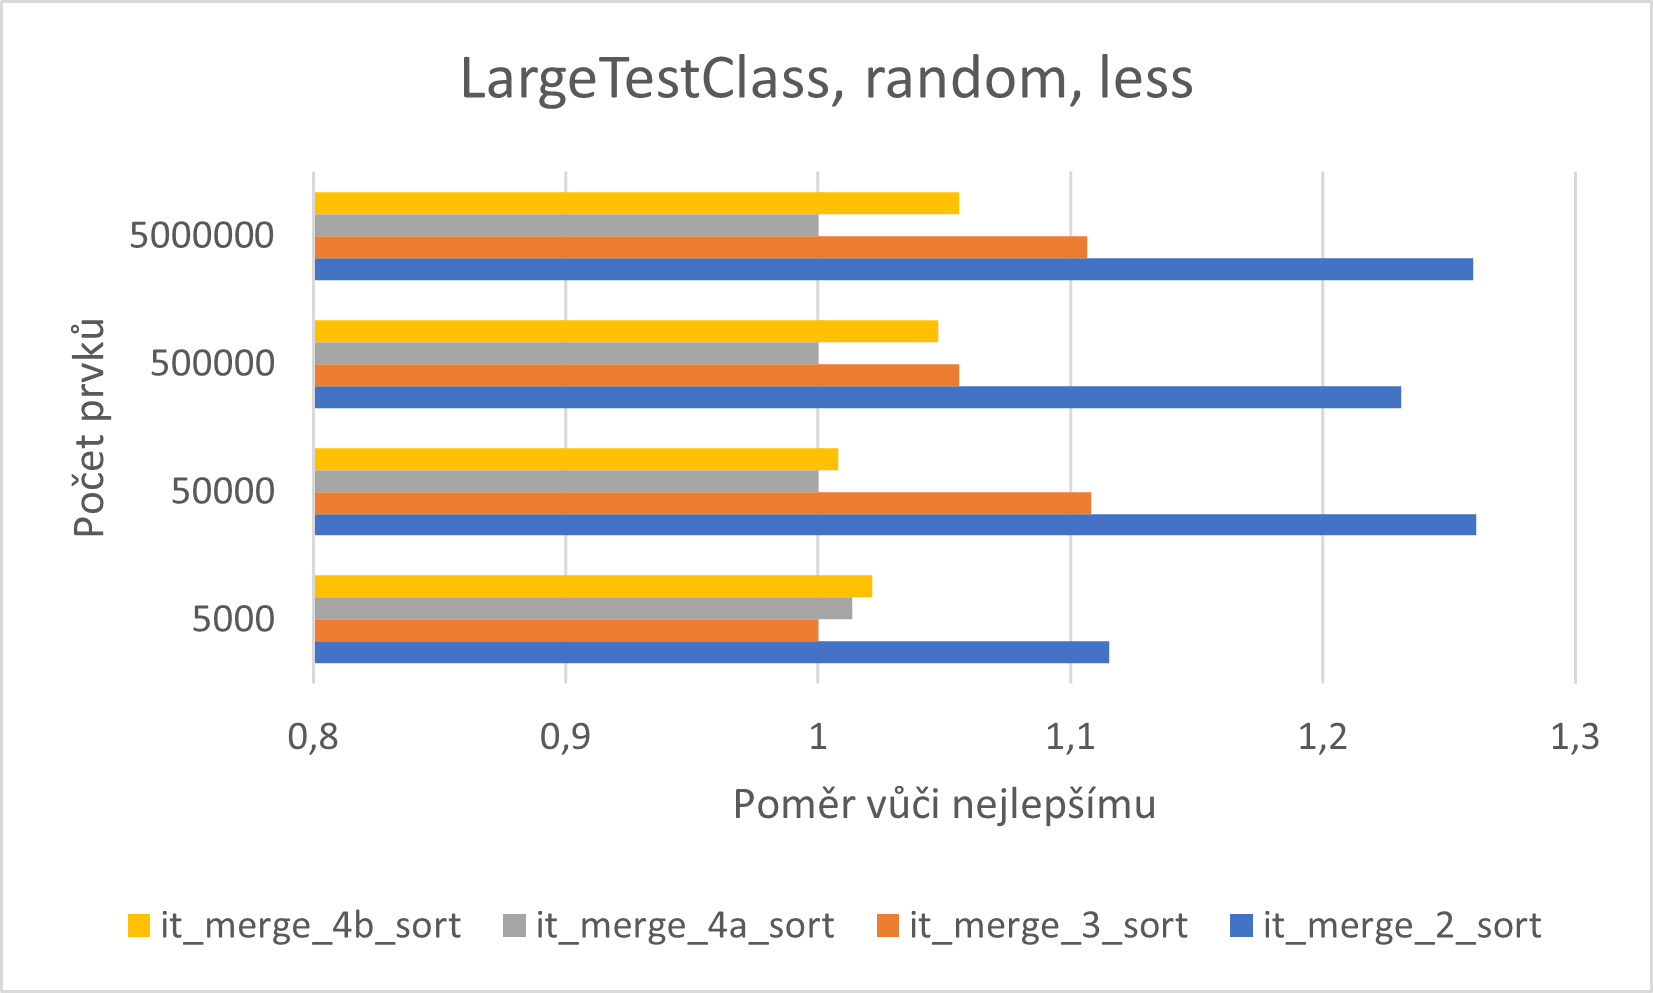
\includegraphics{obrazky/graf17.png}
	\caption[Porovnání algoritmů it\_merge\_4b\_sort, it\_merge\_4a\_sort,\linebreak it\_merge\_3\_sort a it\_merge\_3\_sort na náhodných datech typu LargeTestClass]{Porovnání algoritmů it\_merge\_4b\_sort, it\_merge\_4a\_sort, it\_merge\_3\_sort a it\_merge\_3\_sort na náhodných datech typu\linebreak LargeTestClass}\label{fig:graf17}
\end{figure}

\begin{figure}[htbp]\centering
	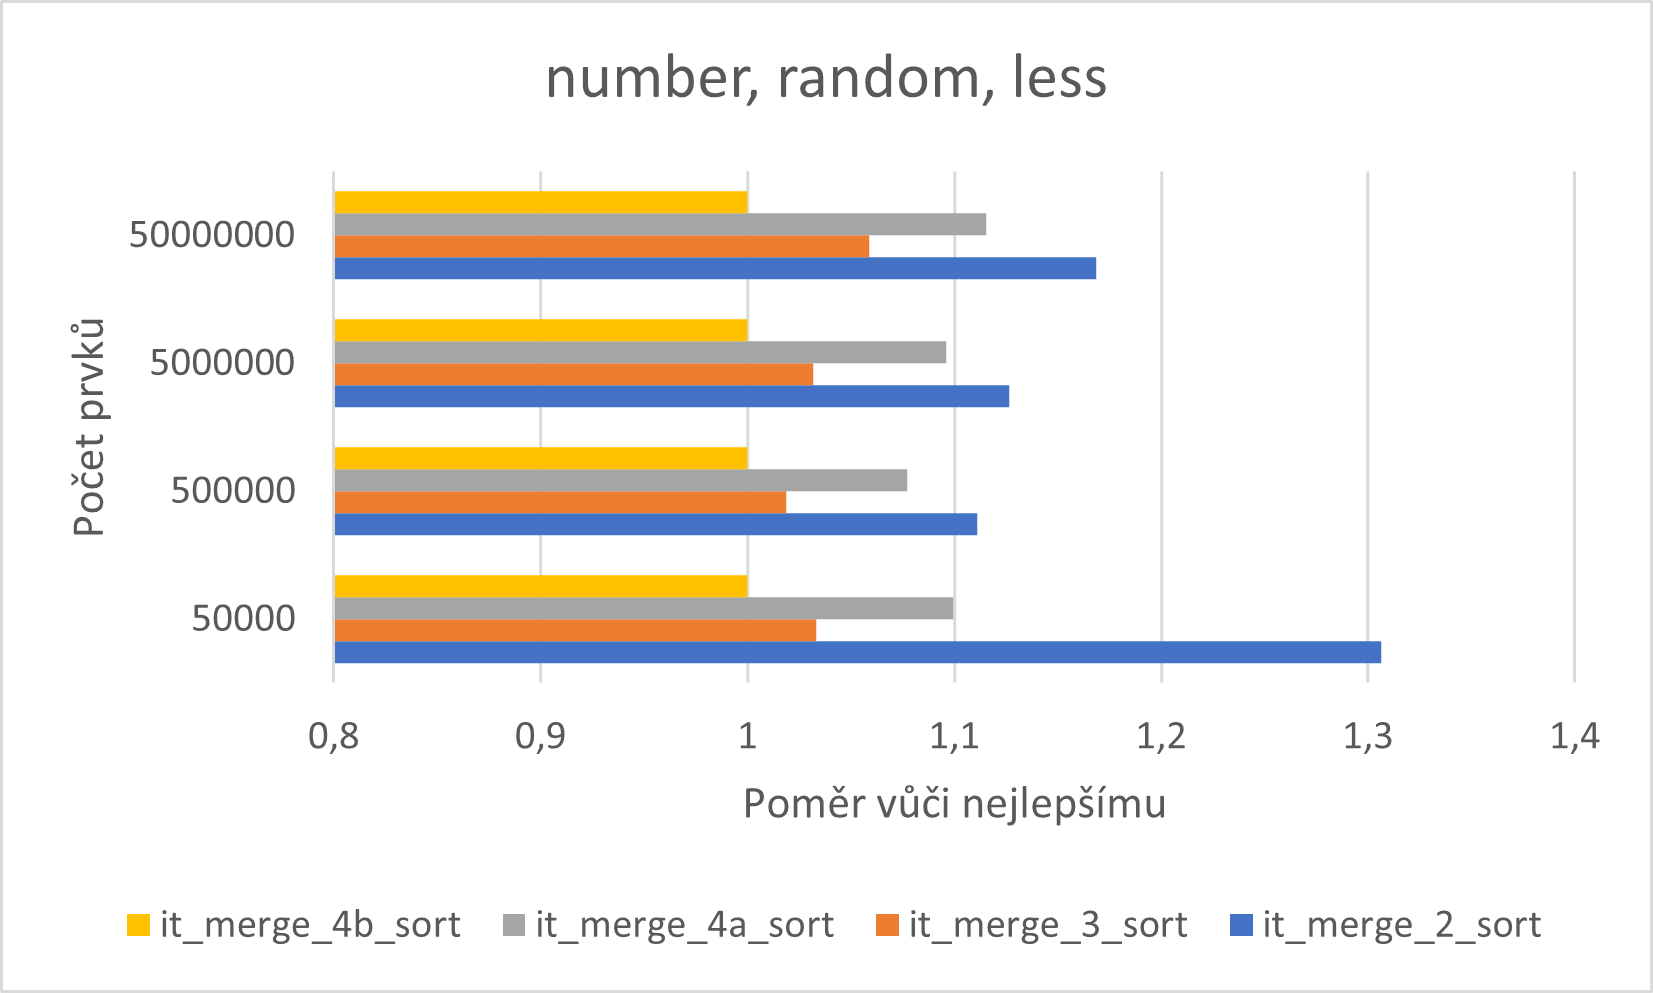
\includegraphics{obrazky/graf18.png}
	\caption[Porovnání algoritmů it\_merge\_4b\_sort, it\_merge\_4a\_sort,\linebreak it\_merge\_3\_sort a it\_merge\_3\_sort na náhodných datech typu integer]{Porovnání algoritmů it\_merge\_4b\_sort, it\_merge\_4a\_sort, it\_merge\_3\_sort a it\_merge\_3\_sort na náhodných datech typu integer}\label{fig:graf18}
\end{figure}

\begin{figure}[htbp]\centering
	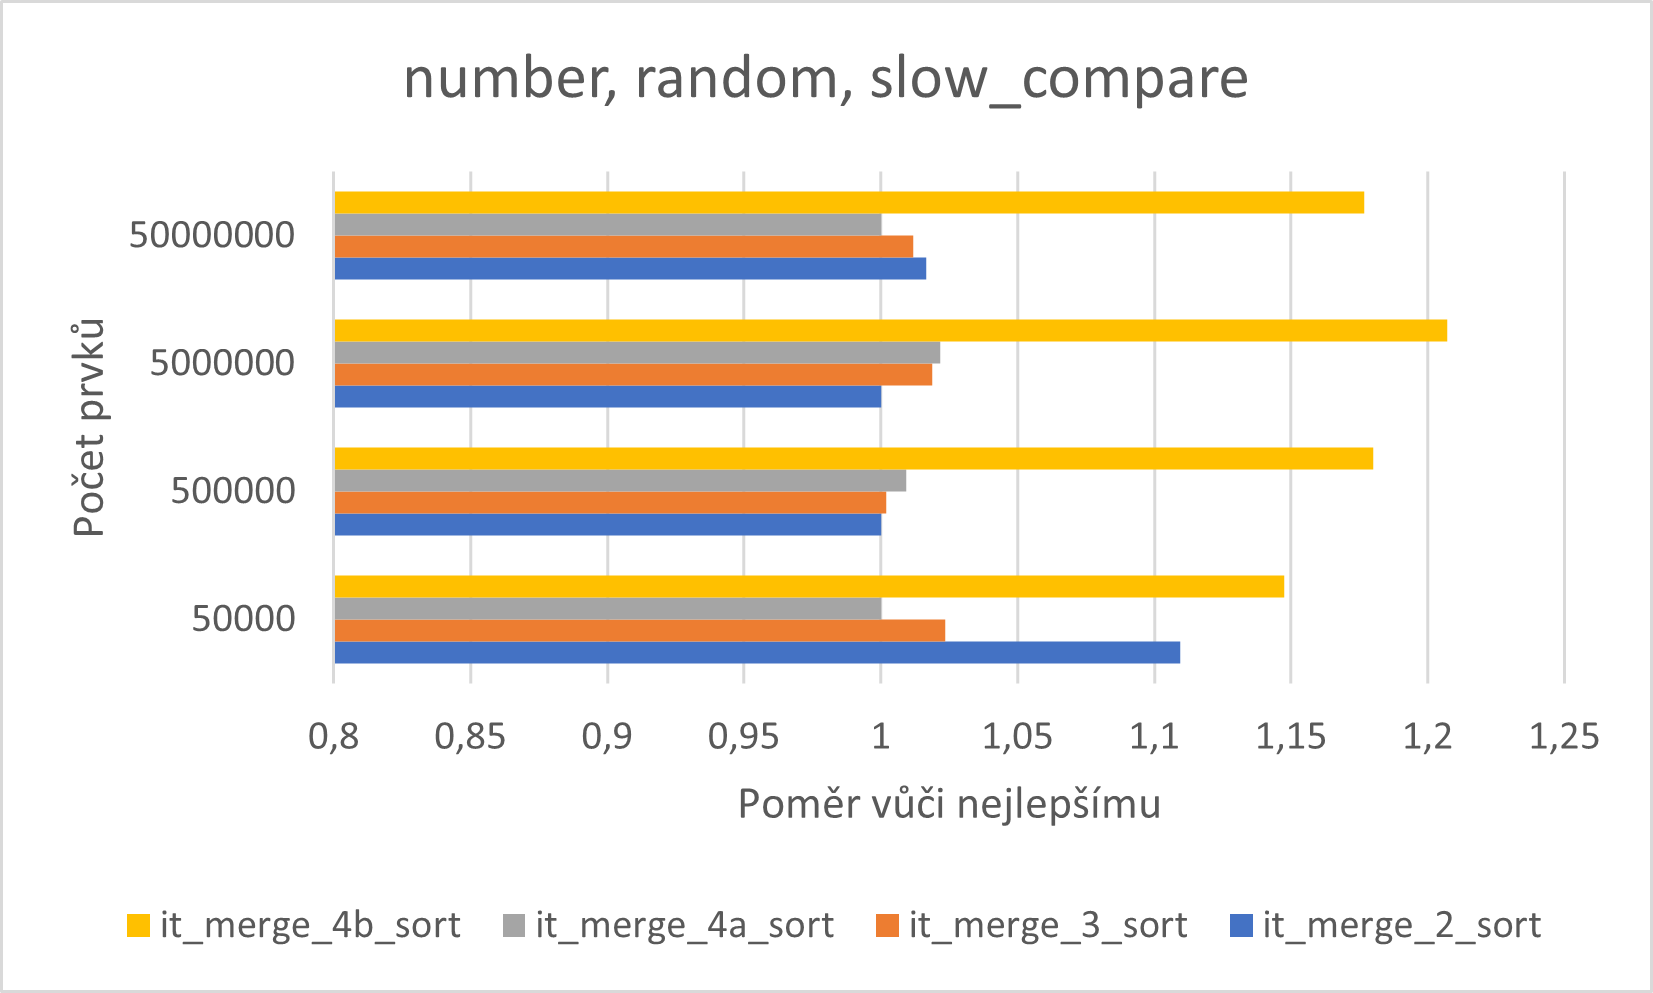
\includegraphics{obrazky/graf19.png}
	\caption[Porovnání algoritmů it\_merge\_4b\_sort, it\_merge\_4a\_sort,\linebreak it\_merge\_3\_sort a it\_merge\_3\_sort na náhodných datech typu integer pomocí slow\_compare]{Porovnání algoritmů it\_merge\_4b\_sort, it\_merge\_4a\_sort, it\_merge\_3\_sort a it\_merge\_3\_sort na náhodných datech typu integer pomocí slow\_compare}\label{fig:graf19}
\end{figure}

\begin{table}[htbp]\centering
 	\caption[Porovnání počtu porovnání algoritmů it\_merge\_2\_sort,\linebreak it\_merge\_3\_sort, it\_merge\_4a\_sort a it\_merge\_4b\_sort]{Porovnání počtu porovnání algoritmů it\_merge\_2\_sort, it\_merge\_3\_sort, it\_merge\_4a\_sort a it\_merge\_4b\_sort}\label{tab:tab3}
 	\begin{tabular}{|c|c|c|c|c|}\hline 
 	& \multicolumn{4}{c|}{prvků} \tabularnewline \hline
algoritmus & 50000 & 500000 & 5000000 & 50000000 \tabularnewline \hline\hline
it\_merge\_2\_sort & 714211 & 8807412 & 104751146 & 1212802980 \tabularnewline \hline
it\_merge\_3\_sort & 879242 & 11093638 & 132730581 & 1504735394 \tabularnewline \hline
it\_merge\_4a\_sort & 714211 & 9275307 & 109670298 & 1212814976 \tabularnewline \hline
it\_merge\_4b\_sort & 962129 & 12742307 & 154269783 & 1710706481 \tabularnewline \hline

	\end{tabular}
\end{table}

Vzhledem k využití Timsortu k řazení převážně neprimitivních typů by bylo nejlepší použít algoritmus z \texttt{it\_merge\_4a\_sortu}. Došlo by tím pravděpodobně k malému zrychlení. Pokud bychom chtěli zrychlit primitivní typy, pak se nabízí využití \texttt{it\_merge\_3\_sort} nebo \texttt{it\_merge\_4b\_sort}.

Ať už bychom si vybrali kterýkoliv z těchto algoritmů, přišli bychom tím o možnost využívat invariantů k ušetření paměti. Všechny runy by se pravděpodobně musely najít najednou, protože režie kontroly nových invariantů by mohla být moc velká.

Při porovnávání různých řadících funkcí těchto algoritmů jsem si všiml, že funkce \texttt{less} je pomalejší než \texttt{my\_compare} pro LargeTestClass náhodná data (tabulka \ref{tab:tab4}), kromě testu s 5000000 prvky. Mohlo by tedy být zajímavé zkoumat jaký vliv má funkce \texttt{less} na rychlost porovnávání dat různých typů.


 \begin{table}[htbp]\centering
 	\caption[Poměr doby běhu porovnávacích funkcí less a my\_compare]{Poměr doby běhu porovnávacích funkcí less a my\_compare}\label{tab:tab4}
 	\begin{tabular}{|c|c|c|c|c|}\hline
 		prvků		& algoritmus		& less	& my\_compare & less/my\_compare	\tabularnewline \hline \hline
5000 & it\_merge\_2\_sort & 2513 & 2204 & 1,1401 \tabularnewline \hline
5000 & it\_merge\_3\_sort & 2253 & 2064 & 1,0915 \tabularnewline \hline
5000 & it\_merge\_4a\_sort & 2283 & 1937 & 1,1786 \tabularnewline \hline
5000 & it\_merge\_4b\_sort & 2301 & 2060 & 1,1169 \tabularnewline \hline
50000 & it\_merge\_2\_sort & 29663 & 21660 & 1,3694 \tabularnewline \hline
50000 & it\_merge\_3\_sort & 26073 & 20523 & 1,2704 \tabularnewline \hline
50000 & it\_merge\_4a\_sort & 23530 & 18610 & 1,2643 \tabularnewline \hline
50000 & it\_merge\_4b\_sort & 23713 & 19589 & 1,2105 \tabularnewline \hline
500000 & it\_merge\_2\_sort & 272373 & 245590 & 1,1090 \tabularnewline \hline
500000 & it\_merge\_3\_sort & 233615 & 229381 & 1,0184 \tabularnewline \hline
500000 & it\_merge\_4a\_sort & 221258 & 210027 & 1,0534 \tabularnewline \hline
500000 & it\_merge\_4b\_sort & 231815 & 230400 & 1,0061 \tabularnewline \hline
5000000 & it\_merge\_2\_sort & 3174058 & 3390263 & 0,9362 \tabularnewline \hline
5000000 & it\_merge\_3\_sort & 2788695 & 2995951 & 0,9308 \tabularnewline \hline
5000000 & it\_merge\_4a\_sort & 2520025 & 2610436 & 0,9653 \tabularnewline \hline
5000000 & it\_merge\_4b\_sort & 2660849 & 2771709 & 0,9600 \tabularnewline \hline


	\end{tabular}
\end{table}

\section{Testování paralelních algoritmů}

Všechny 4 paralelní algoritmy byly testovány s využitím 1, 2, 4, 8, 16 a 20 vláken a porovnány se základním Timsortem. V prvních čtyřech grafech je znázorněno zrychlení algoritmu při náhodných datech v závislosti na počtu vláken a počtu prvků. Můžeme vidět výrazné velmi výrazné zrychlení a to až 6,8-krát při plném využití 20 jader procesoru pro algoritmy \texttt{merge\_sort\_parallel\_a} (graf \ref{fig:graf20}) a \texttt{merge\_sort\_parallel\_b} (graf \ref{fig:graf21}). Algoritmus\linebreak \texttt{timsort\_parallel\_a} (graf \ref{fig:graf22}) dosáhl až pětinásobného zrychlení při 20 vláknech a poslední \texttt{timsort\_parallel\_b} (graf \ref{fig:graf23}) je s 20 vlákny 2,5-krát rychlejší než běžný Timsort.

\begin{figure}[hbp]\centering
	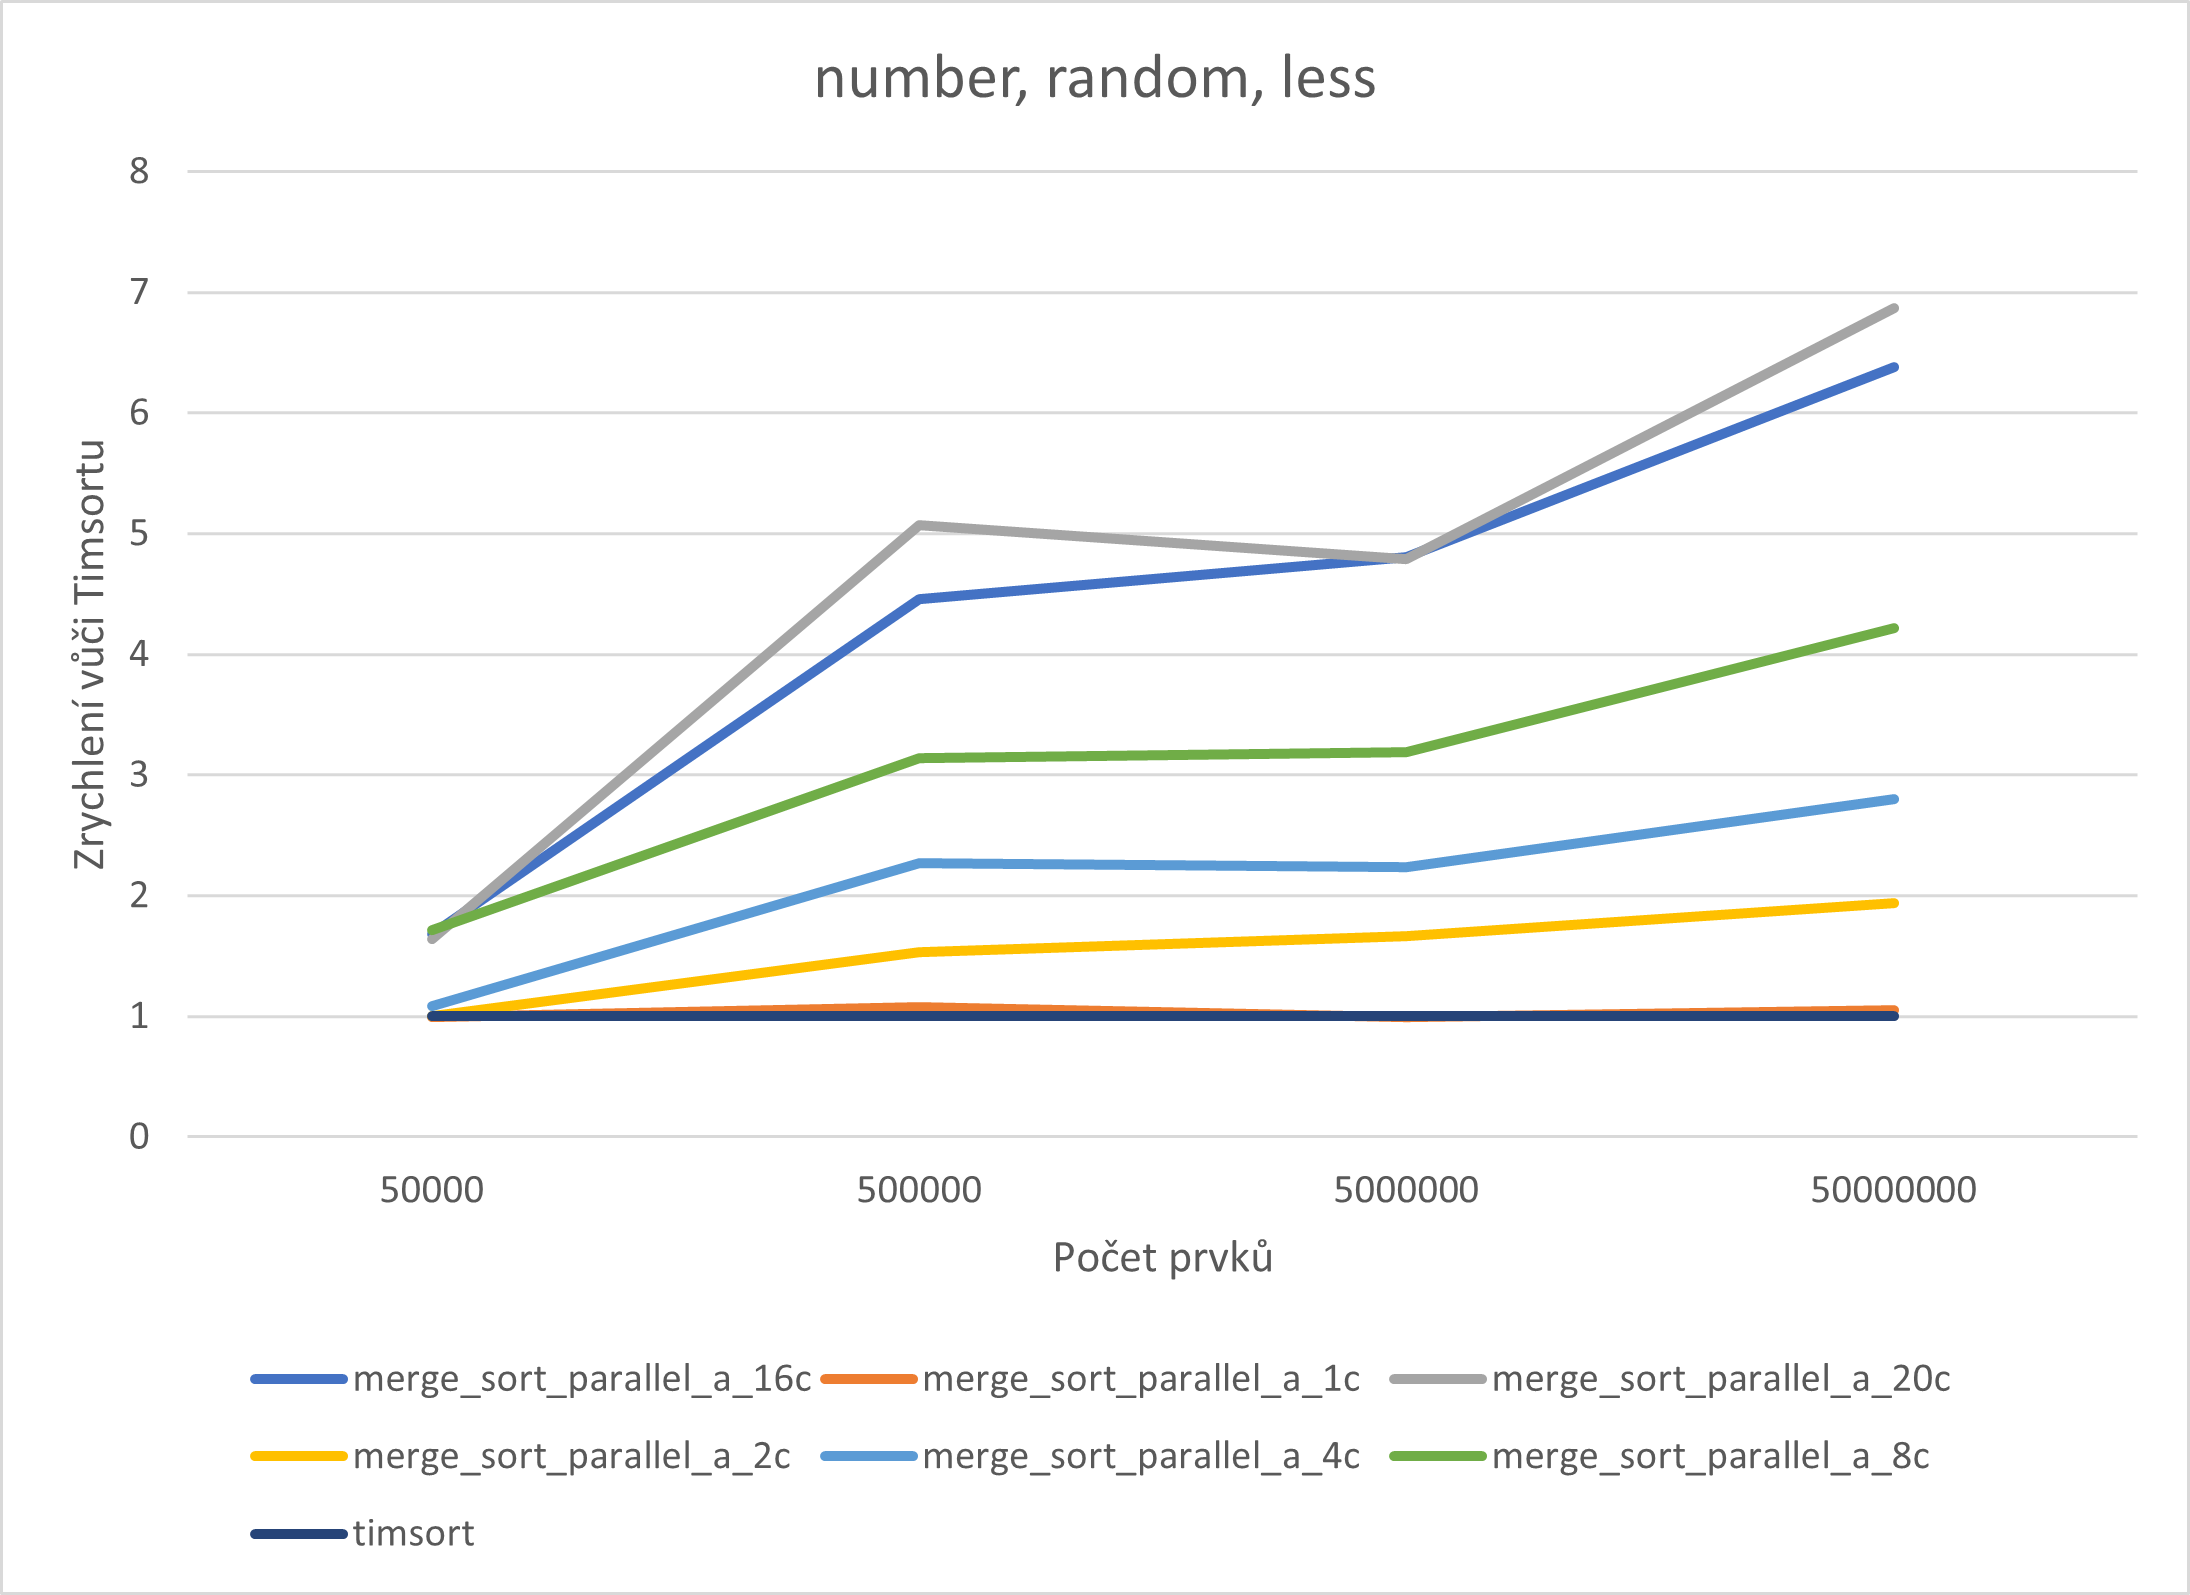
\includegraphics[width=13cm]{obrazky/graf20.png}
	\caption[Zrychlení merge\_sort\_parallel\_a oproti timsortu v závislosti na počtu vláken, náhodná čísla]{Zrychlení merge\_sort\_parallel\_a oproti timsortu v závislosti na počtu vláken, náhodná čísla}\label{fig:graf20}
\end{figure}

\begin{figure}[htbp]\centering
	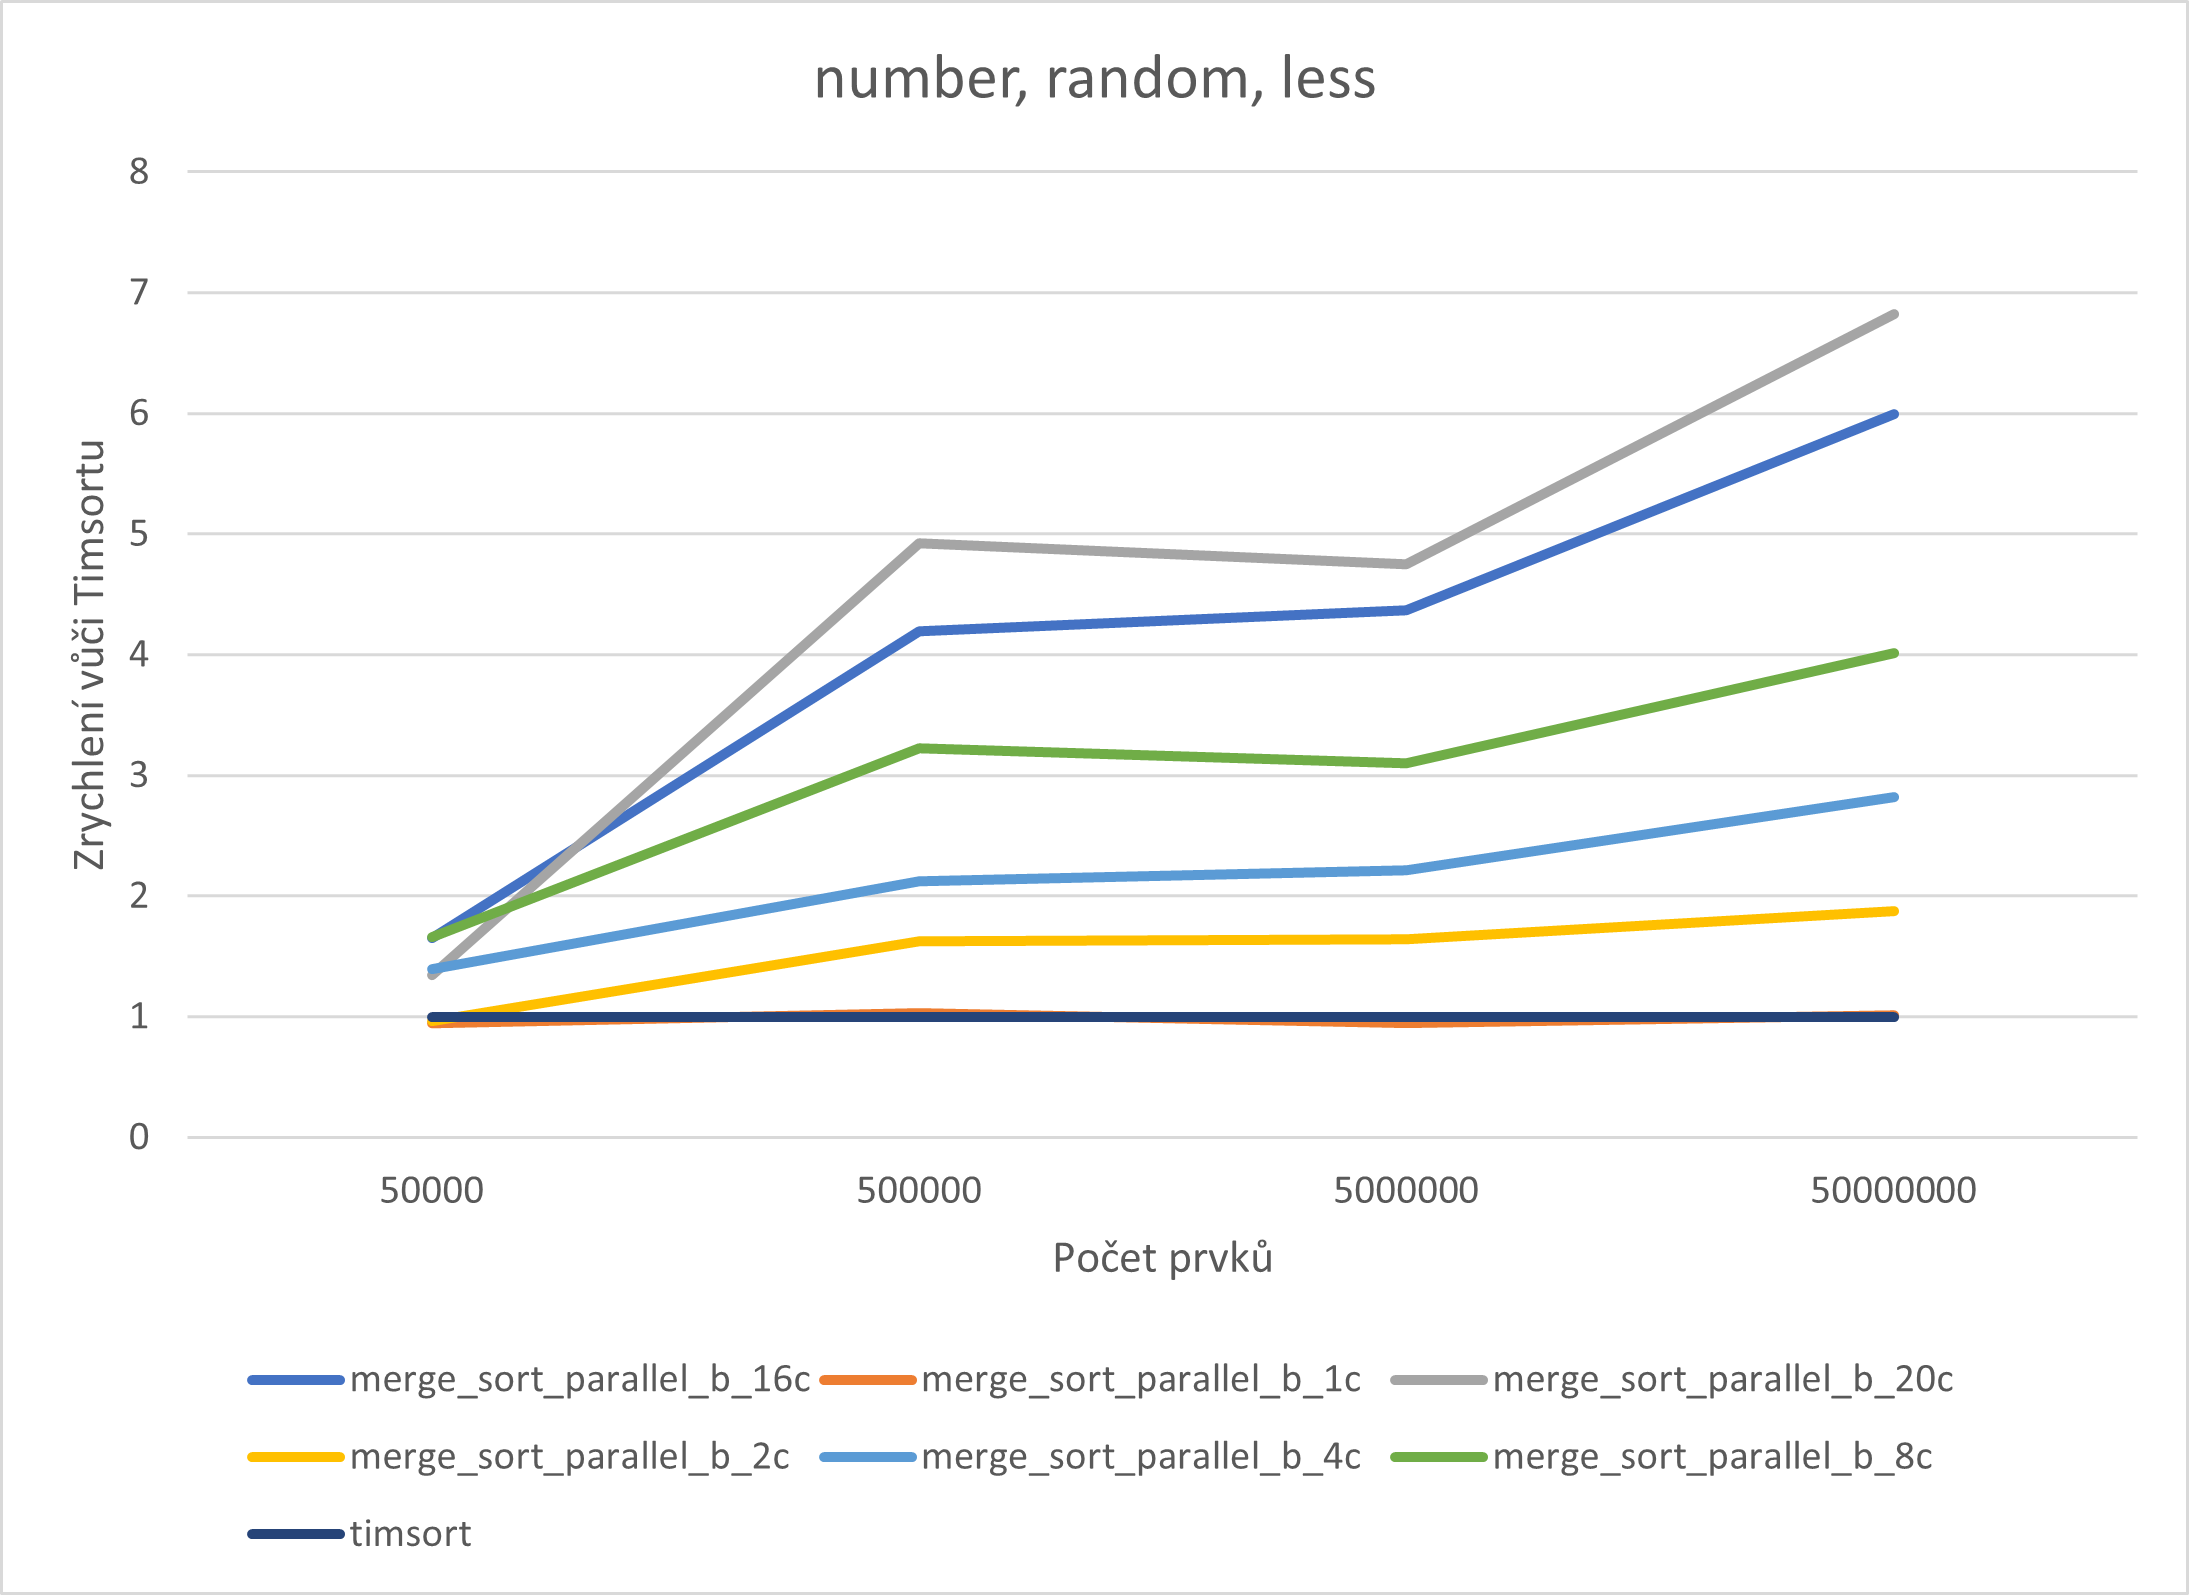
\includegraphics[width=13cm]{obrazky/graf21.png}
	\caption[Zrychlení merge\_sort\_parallel\_b oproti timsortu v závislosti na počtu vláken, náhodná čísla]{Zrychlení merge\_sort\_parallel\_b oproti timsortu v závislosti na počtu vláken, náhodná čísla}\label{fig:graf21}
\end{figure}

\begin{figure}[htbp]\centering
	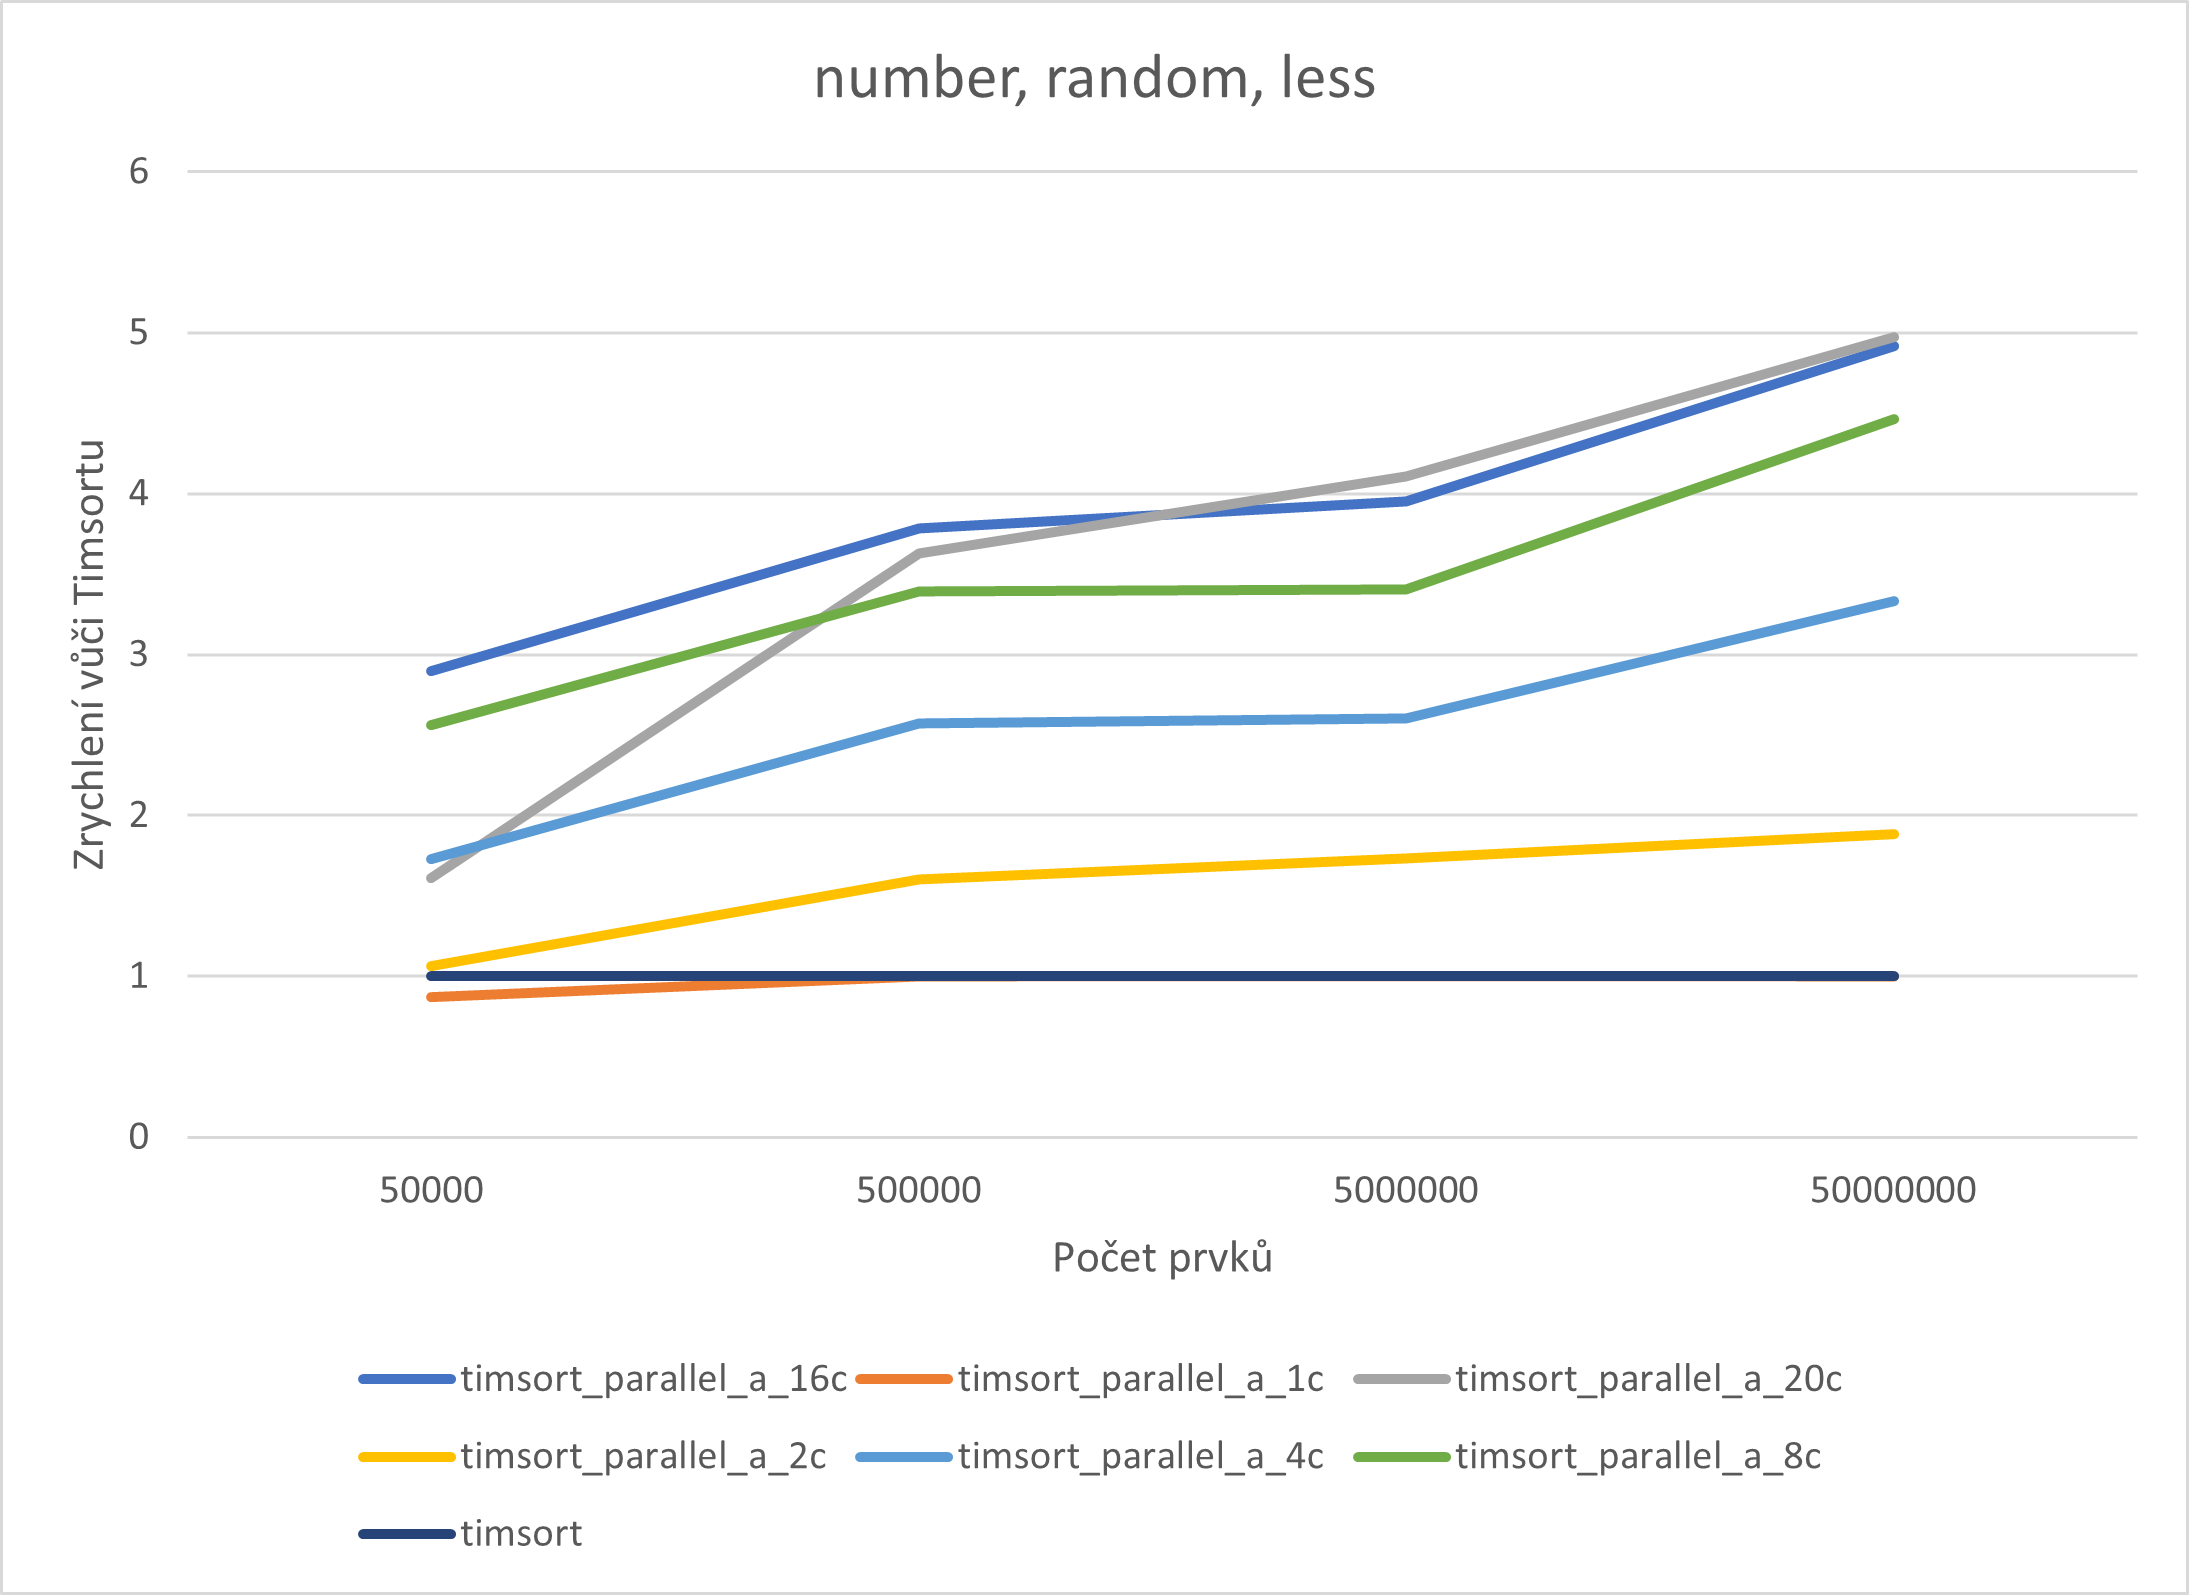
\includegraphics[width=13cm]{obrazky/graf22.png}
	\caption[Zrychlení timsort\_parallel\_a oproti timsortu v závislosti na počtu vláken, náhodná čísla]{Zrychlení timsort\_parallel\_a oproti timsortu v závislosti na počtu vláken, náhodná čísla}\label{fig:graf22}
\end{figure}

\begin{figure}[htbp]\centering
	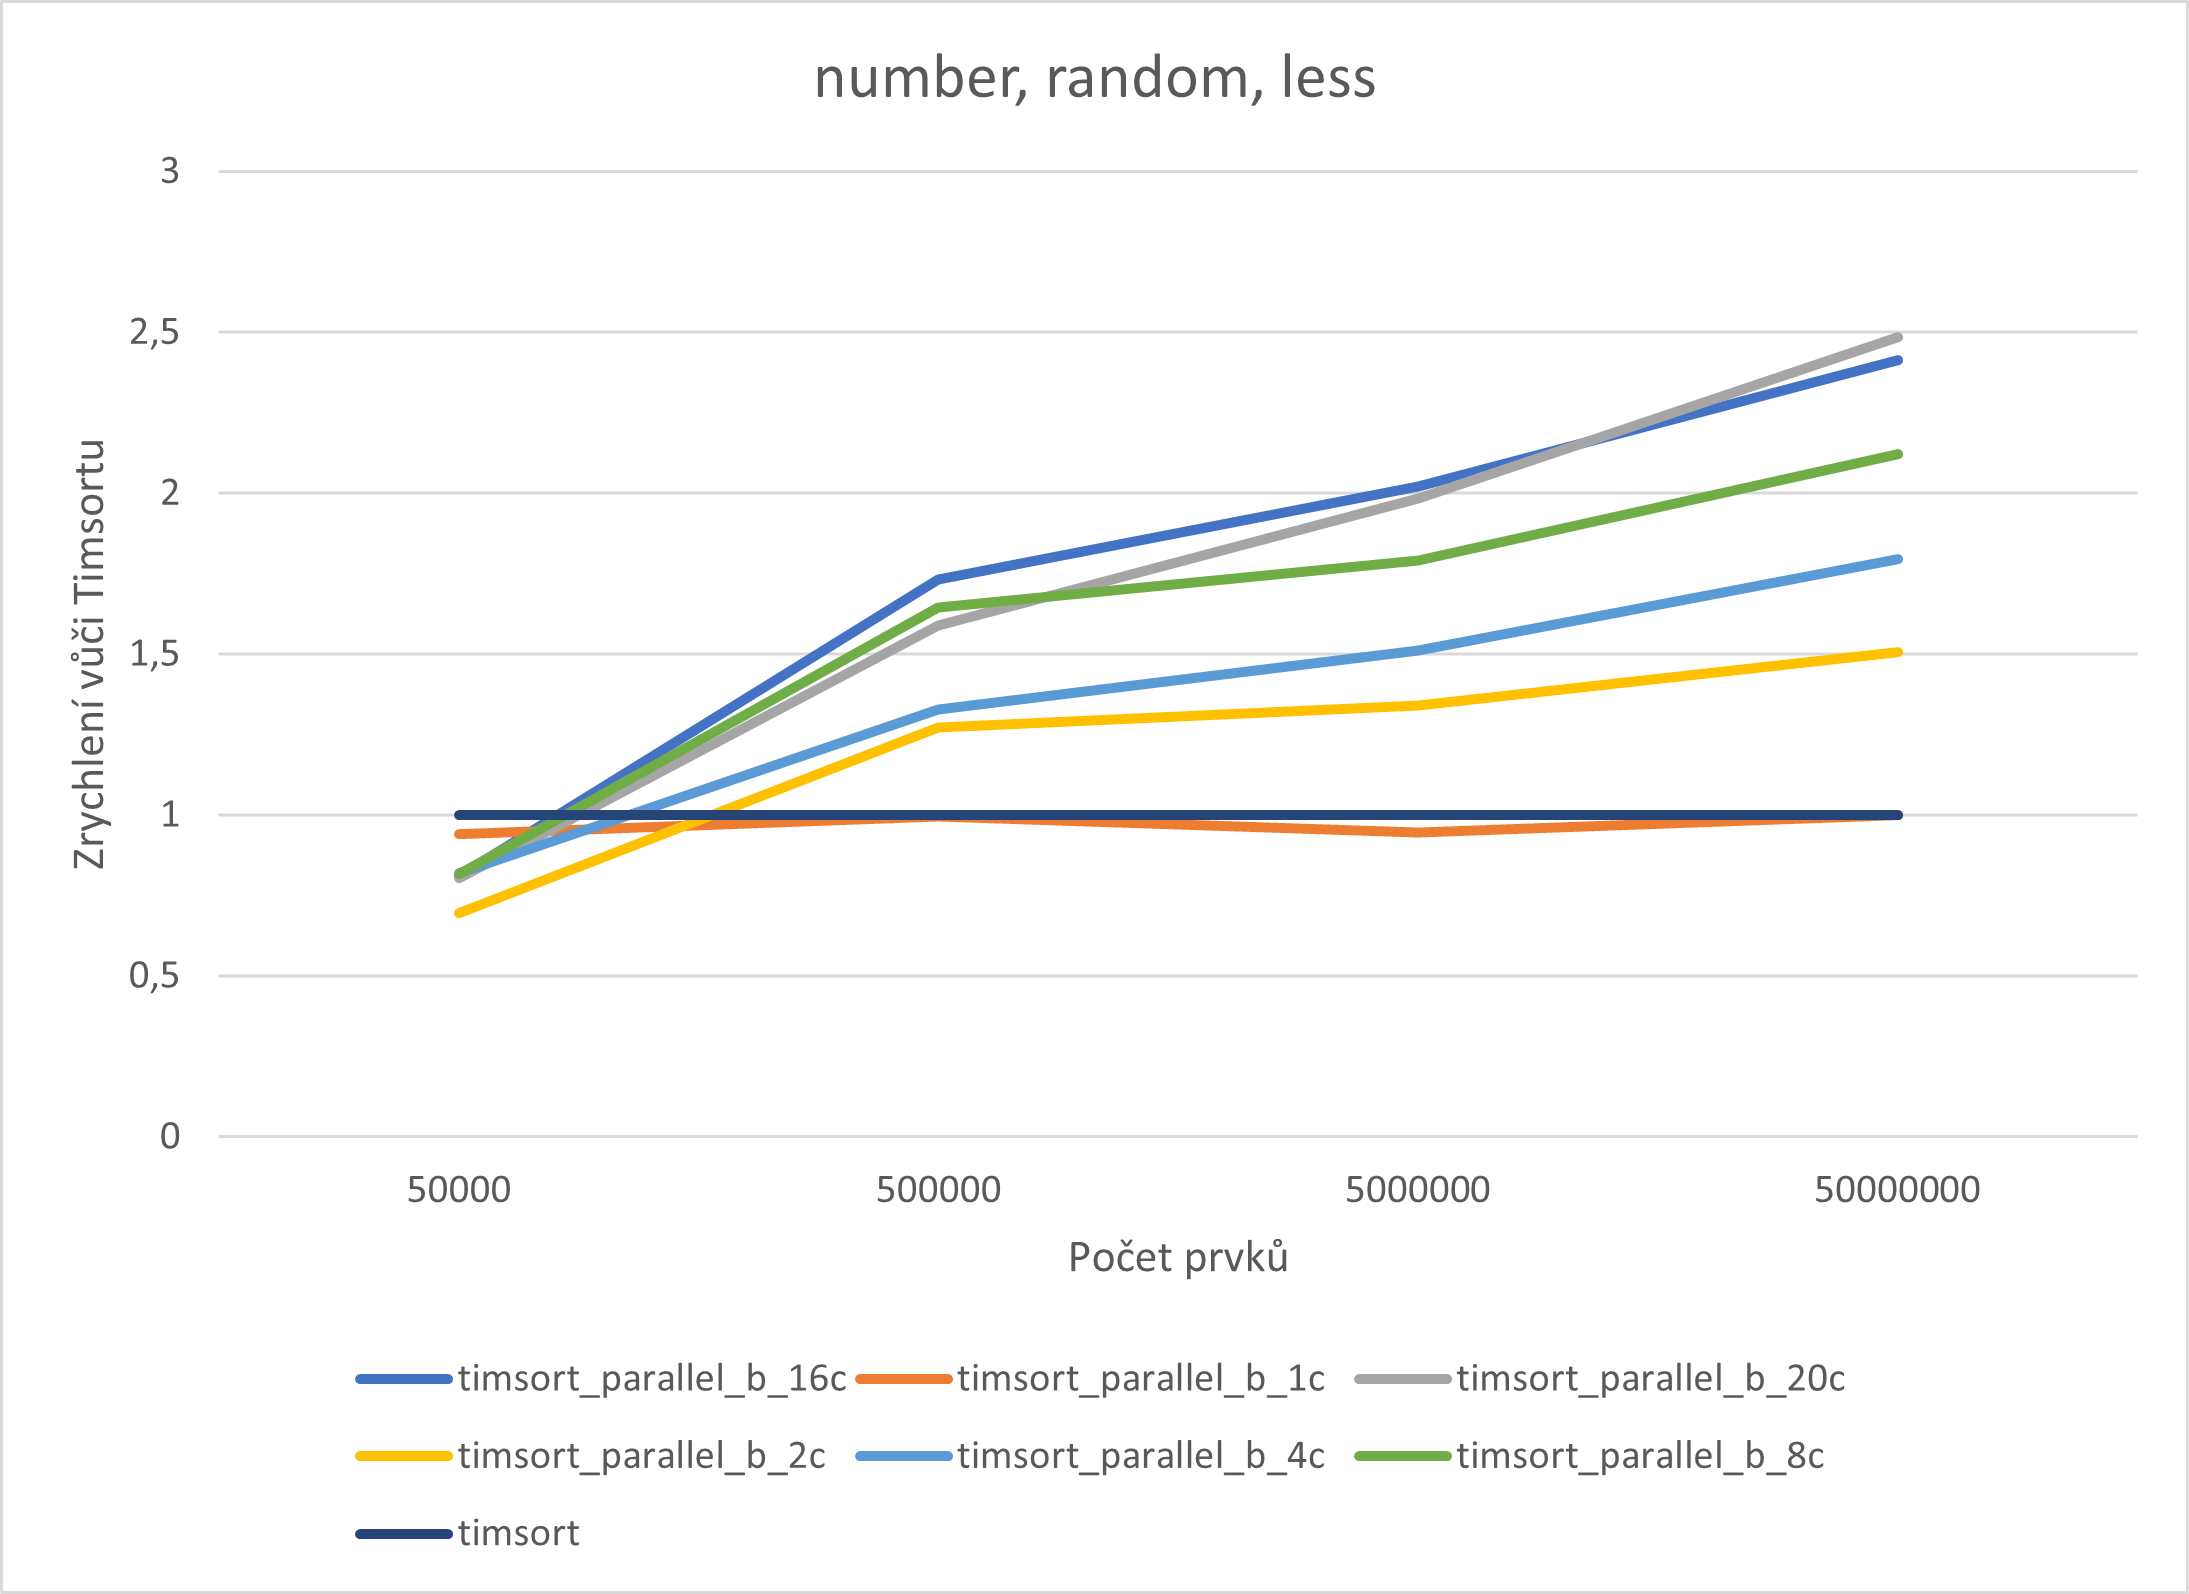
\includegraphics[width=13cm]{obrazky/graf23.png}
	\caption[Zrychlení timsort\_parallel\_b oproti timsortu v závislosti na počtu vláken, náhodná čísla]{Zrychlení timsort\_parallel\_b oproti timsortu v závislosti na počtu vláken, náhodná čísla}\label{fig:graf23}
\end{figure}

Při porovnávání náhodných stringů už je situace jiná. Nejhůře dopadl \texttt{timsort\_parallel\_b} (graf \ref{fig:graf27}), kde i s 20 vlákny je pomalejší než základní Timsort. Ostatní paralelní algoritmy pak byly při 5 milionech prvků a 20 vláknech 2-krát až 3-krát rychlejší než sekvenční Timsort (grafy \ref{fig:graf24}, \ref{fig:graf25}, \ref{fig:graf26}). S alespoň čtyřmi vlákny pak jsou tyto algoritmy stejně rychlé nebo rychlejší než obyčejný Timsort. S jedním vláknem očekáváme, že paralelní algoritmus může být pomalejší, kvůli větší režie okolo samotného řazení. U dvou vláken si můžeme všimnout, že pro více prvků už také dosahujeme zrychlení.

\begin{figure}[htbp]\centering
	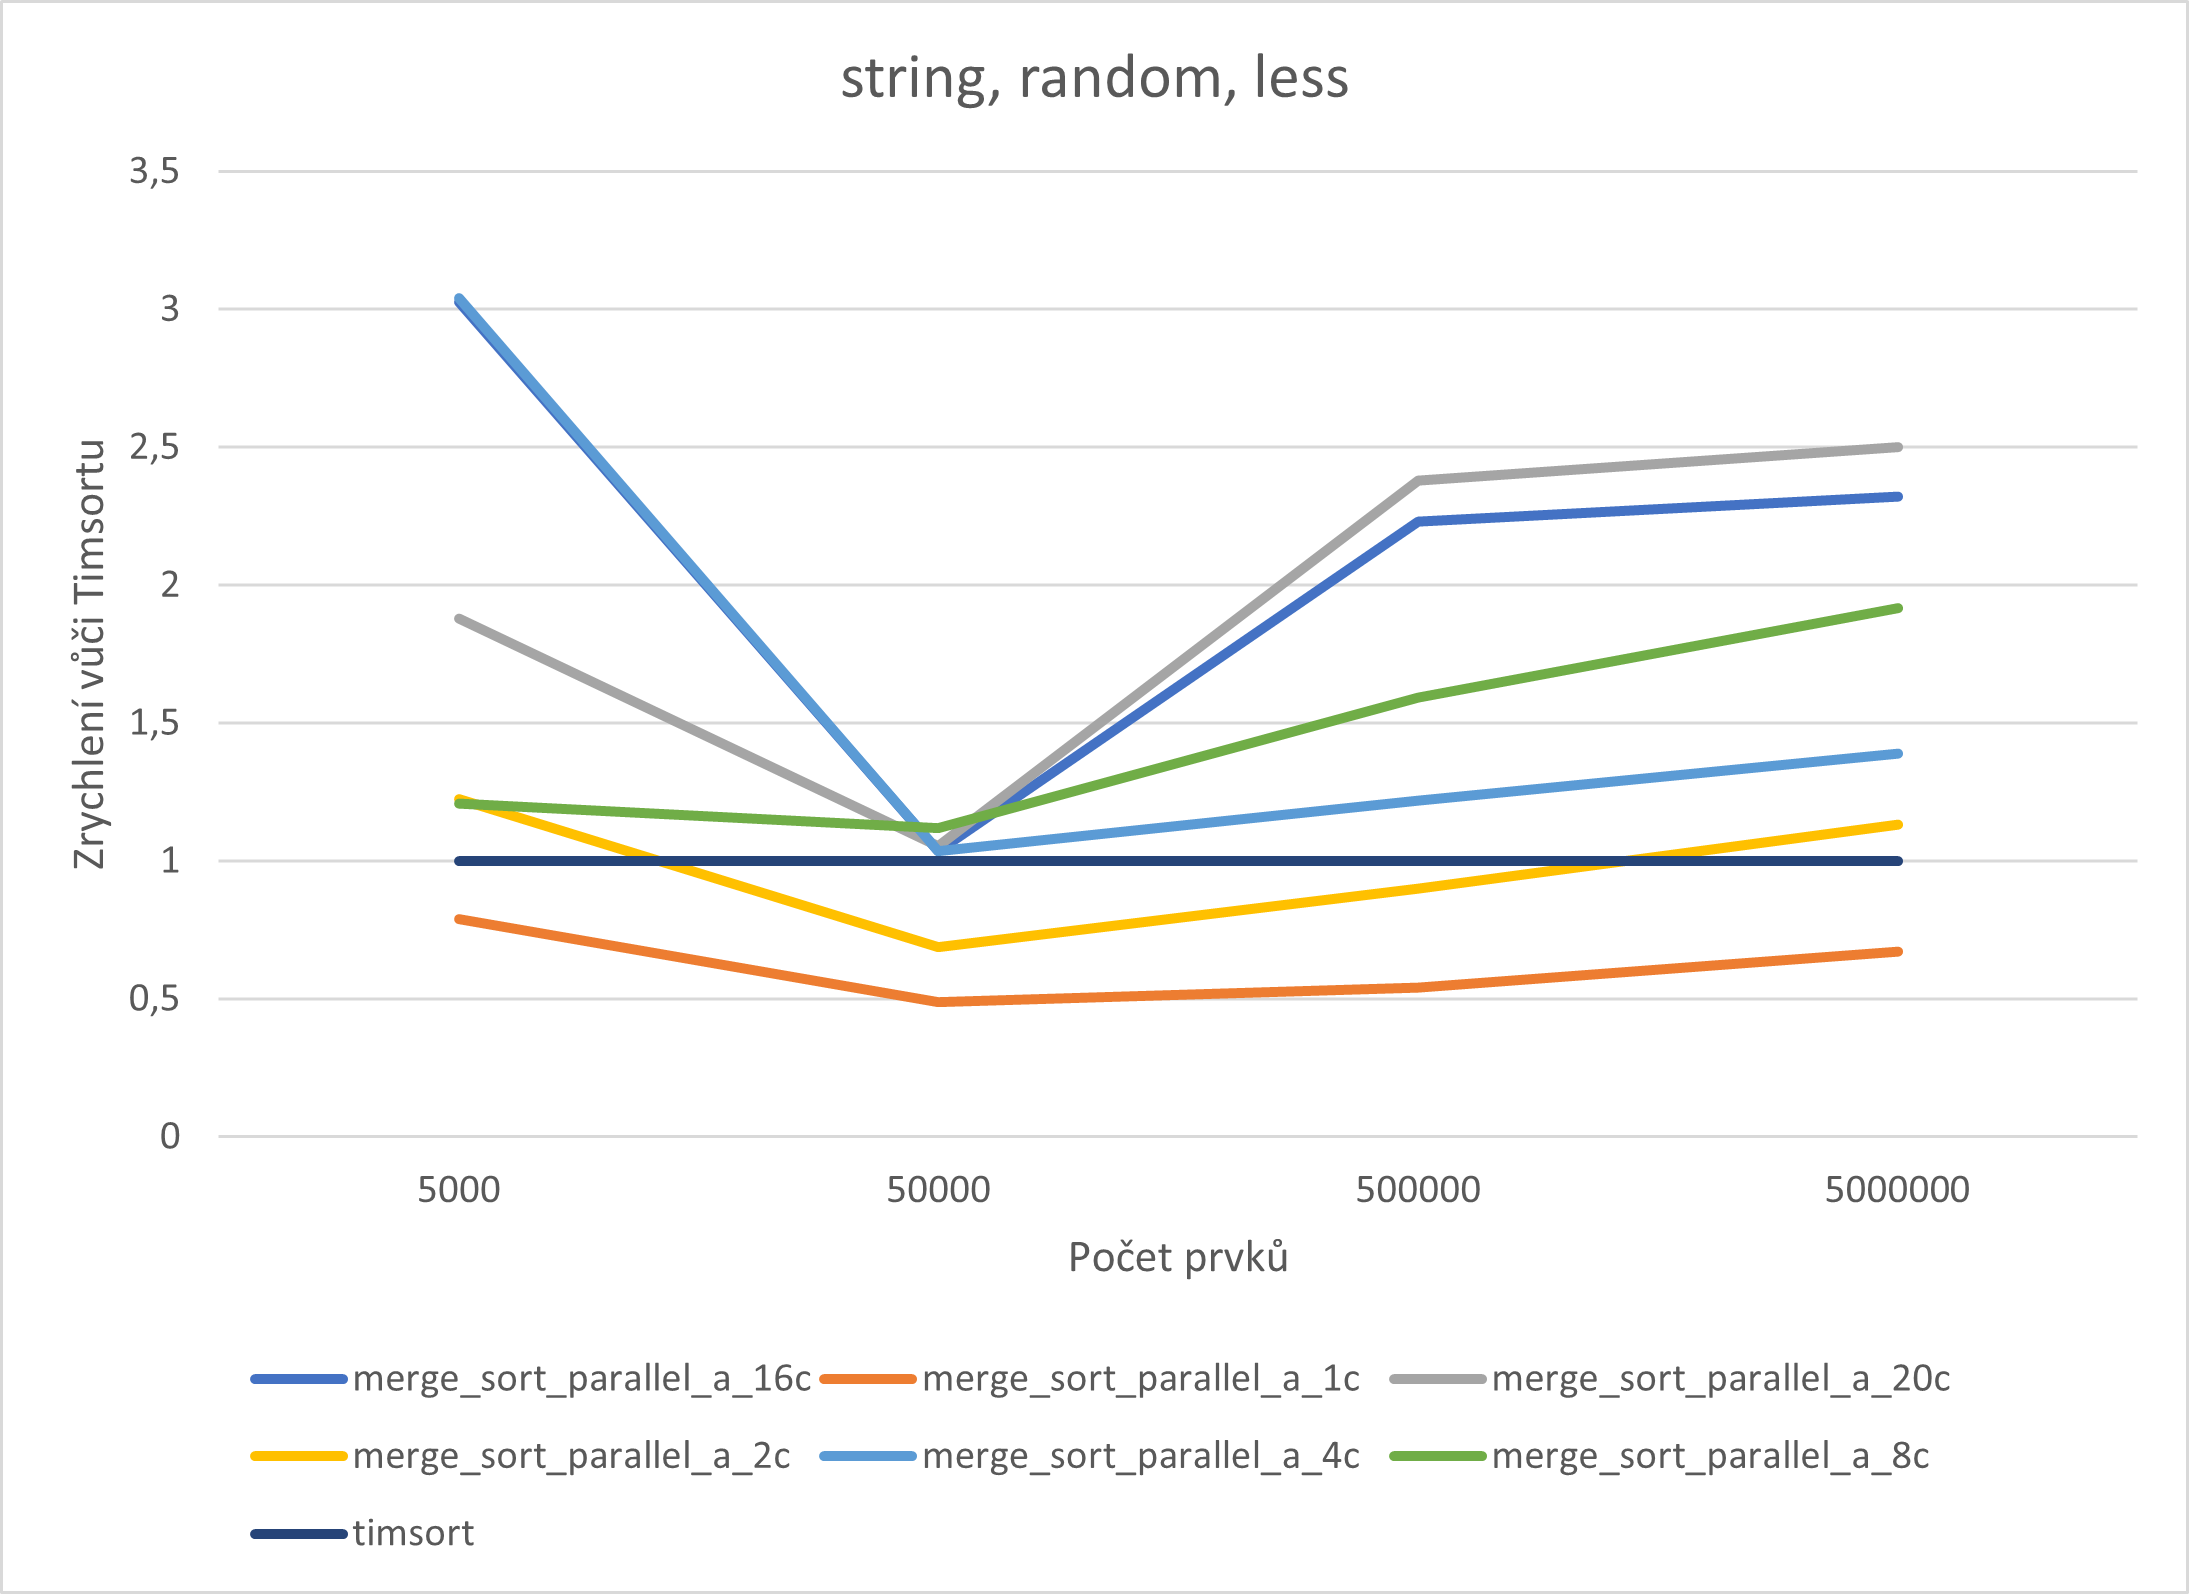
\includegraphics[width=13cm]{obrazky/graf24.png}
	\caption[Zrychlení merge\_sort\_parallel\_a oproti timsortu v závislosti na počtu vláken, náhodné stringy]{Zrychlení merge\_sort\_parallel\_a oproti timsortu v závislosti na počtu vláken, náhodné stringy}\label{fig:graf24}
\end{figure}
\begin{figure}[htbp]\centering
	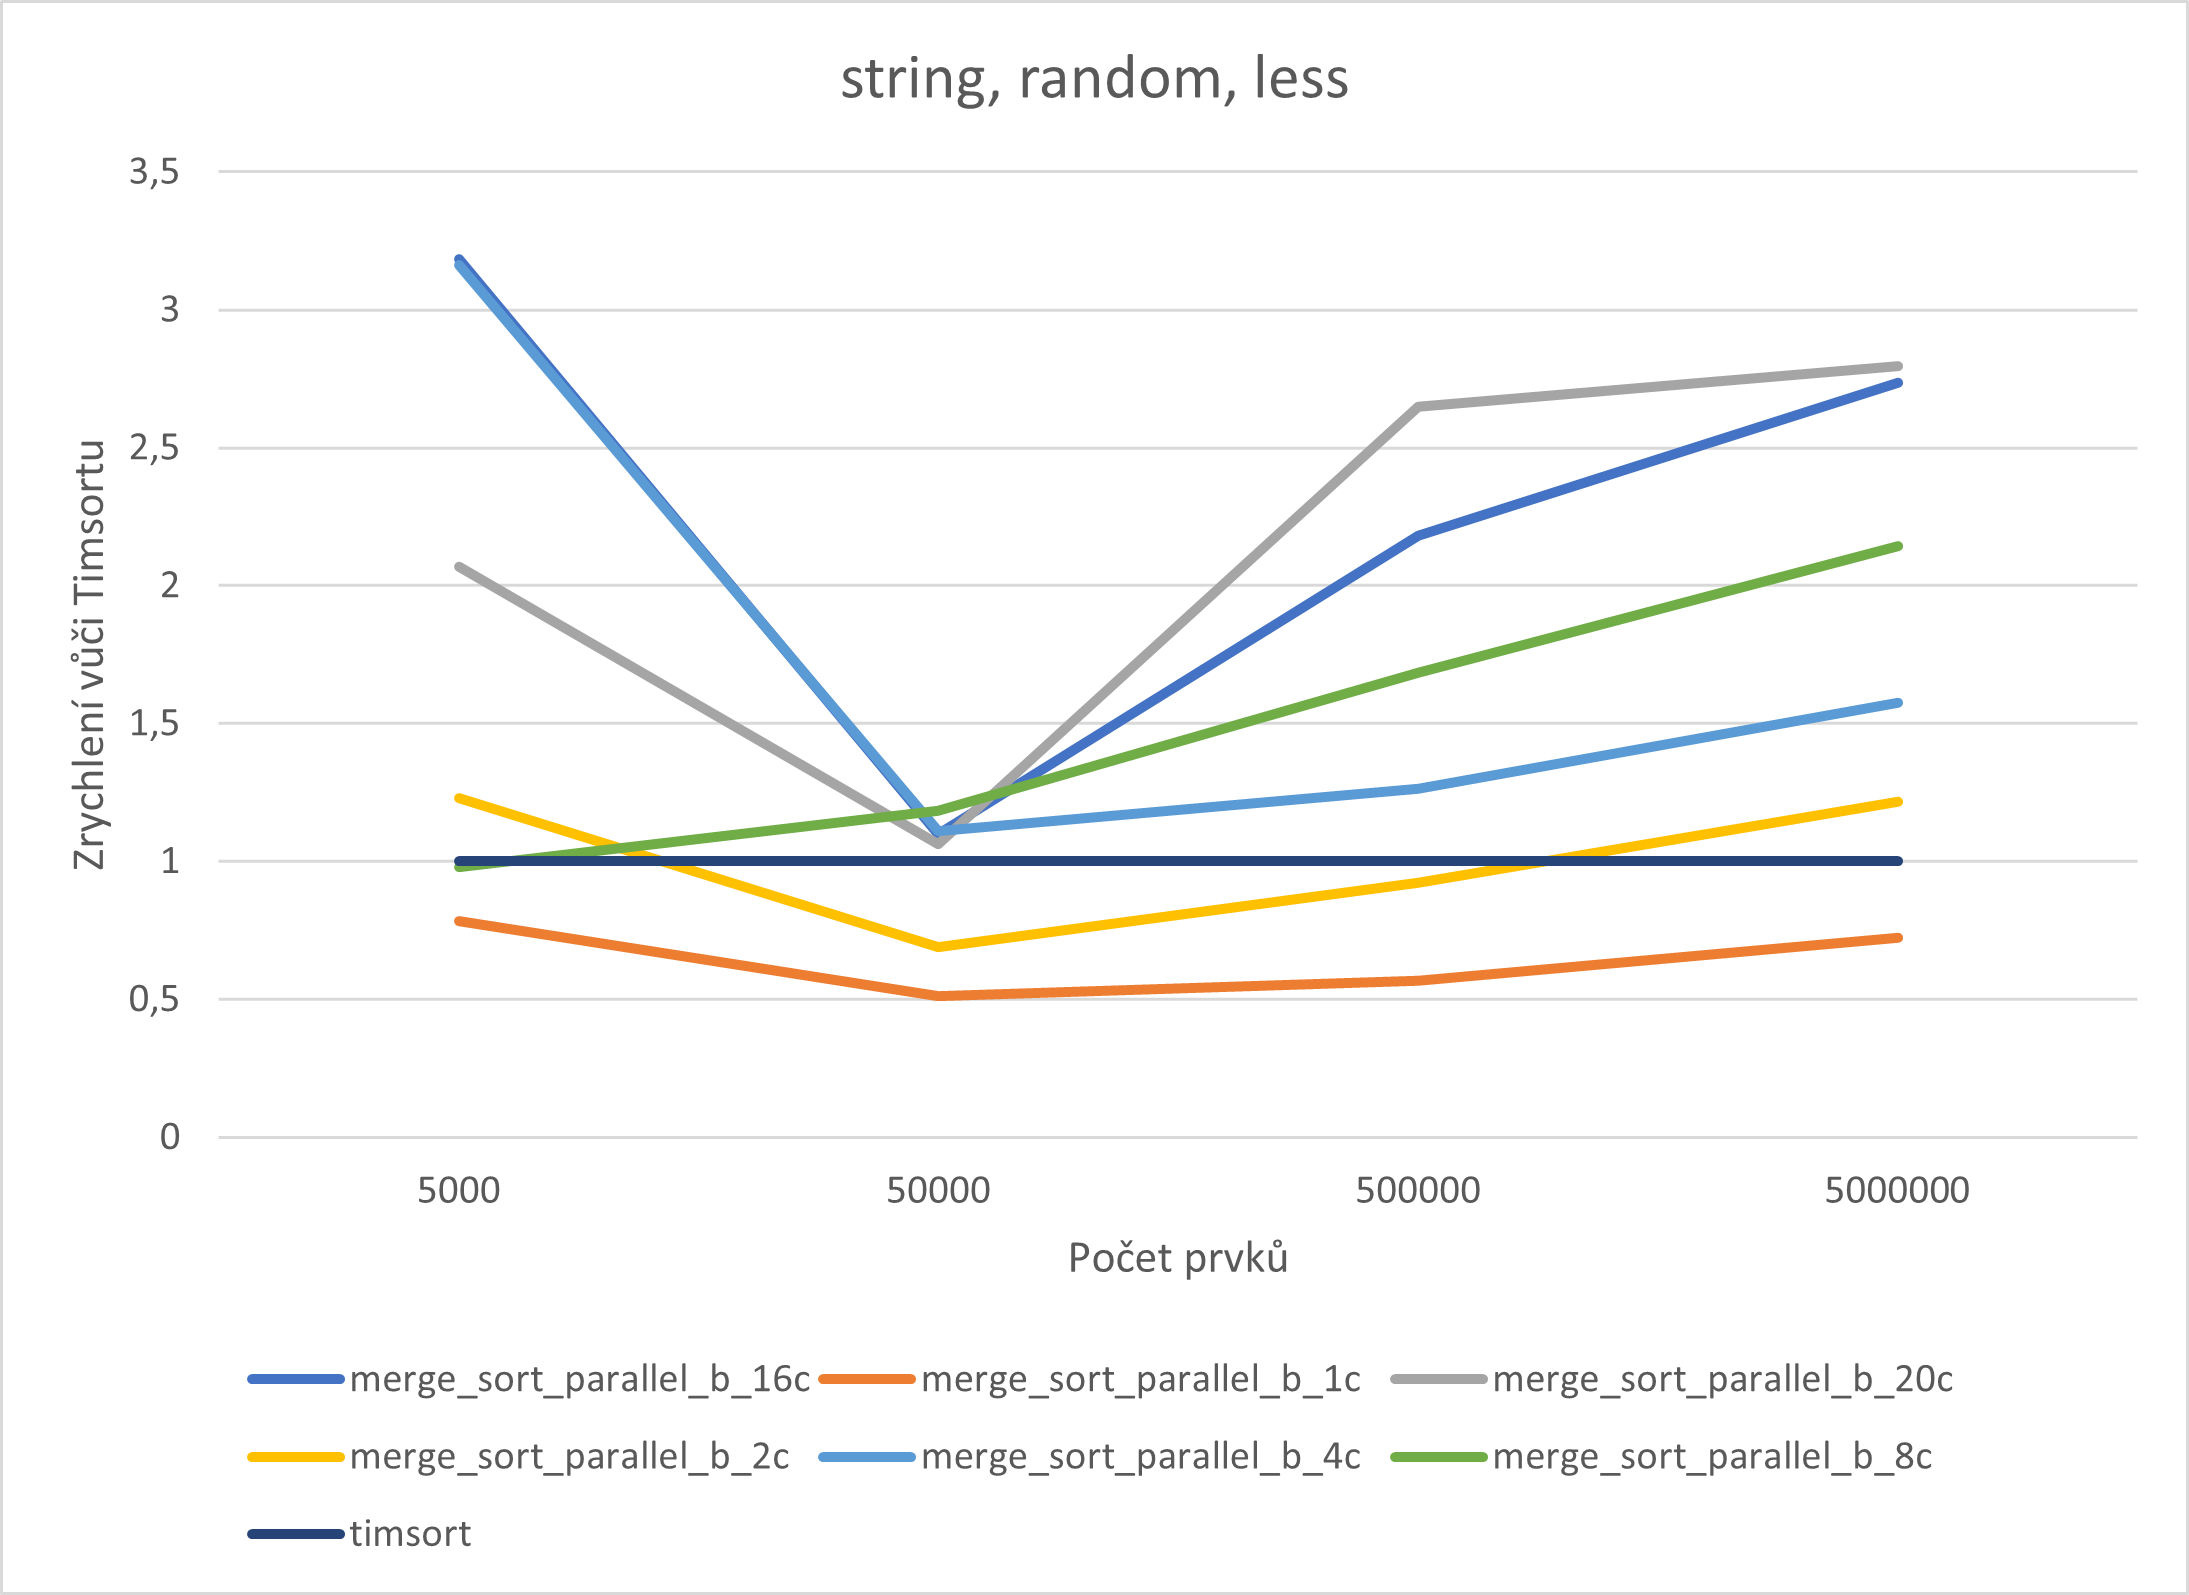
\includegraphics[width=13cm]{obrazky/graf25.png}
	\caption[Zrychlení merge\_sort\_parallel\_b oproti timsortu v závislosti na počtu vláken, náhodné stringy]{Zrychlení merge\_sort\_parallel\_b oproti timsortu v závislosti na počtu vláken, náhodné stringy}\label{fig:graf25}
\end{figure}
\begin{figure}[htbp]\centering
	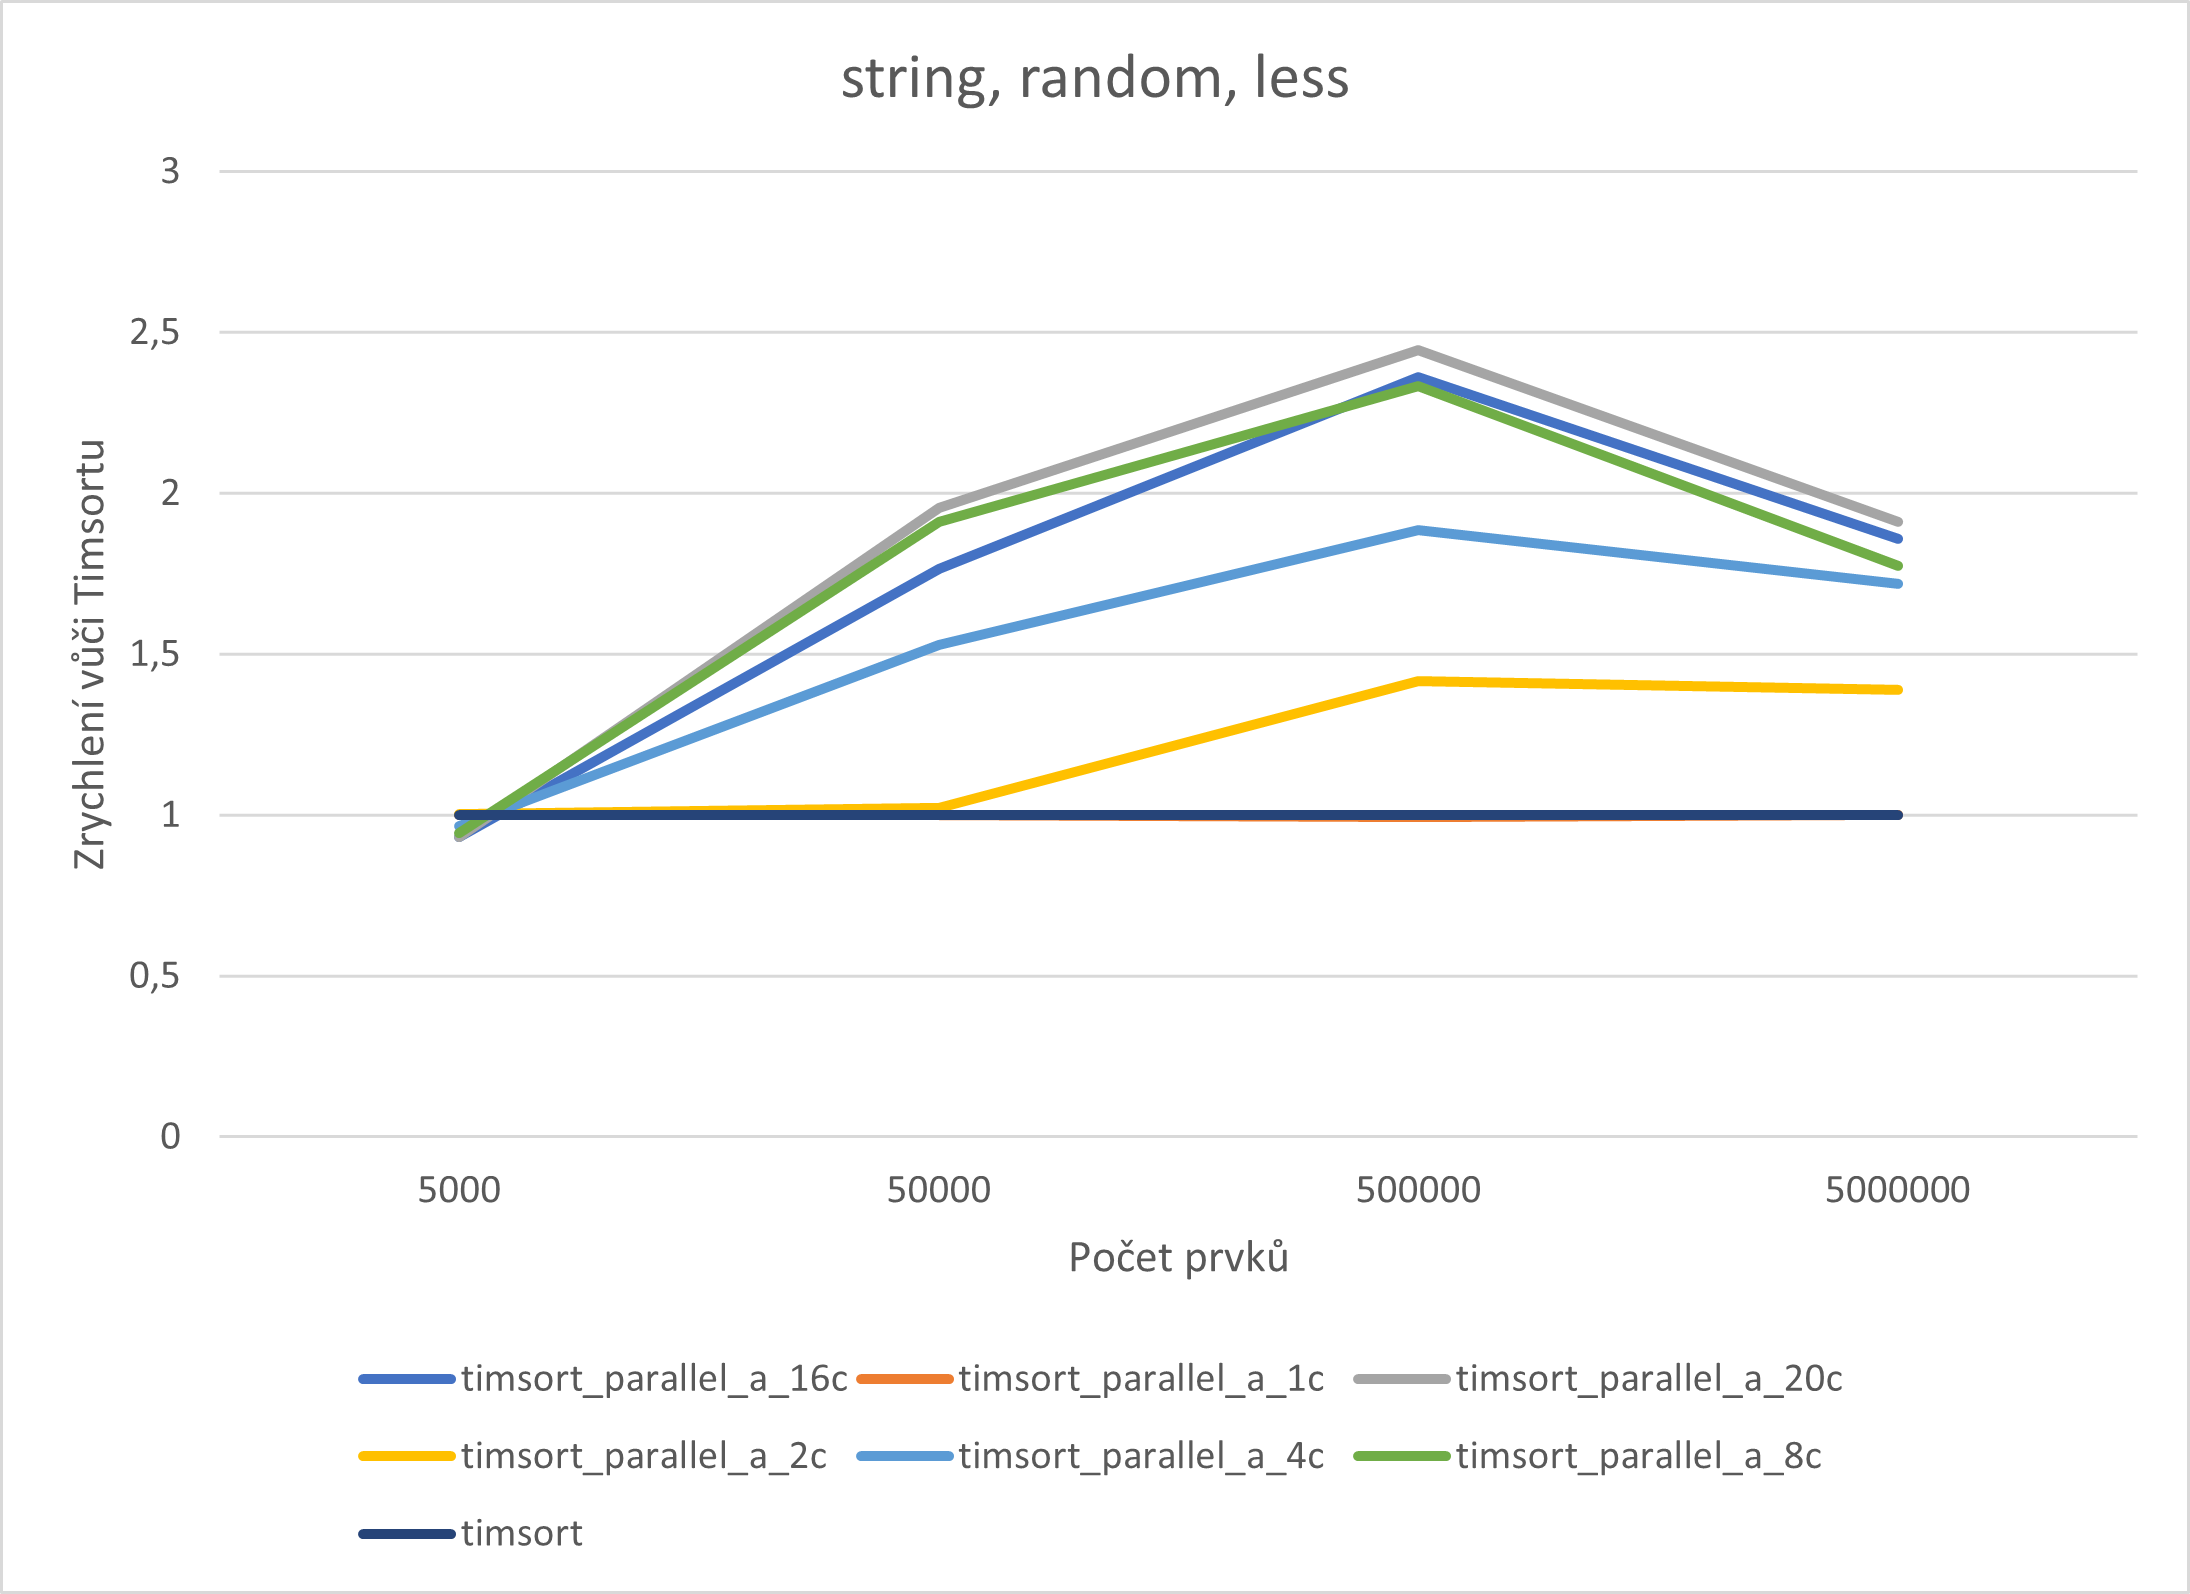
\includegraphics[width=13cm]{obrazky/graf26.png}
	\caption[Zrychlení timsort\_parallel\_a oproti timsortu v závislosti na počtu vláken, náhodné stringy]{Zrychlení timsort\_parallel\_a oproti timsortu v závislosti na počtu vláken, náhodné stringy}\label{fig:graf26}
\end{figure}
\begin{figure}[htbp]\centering
	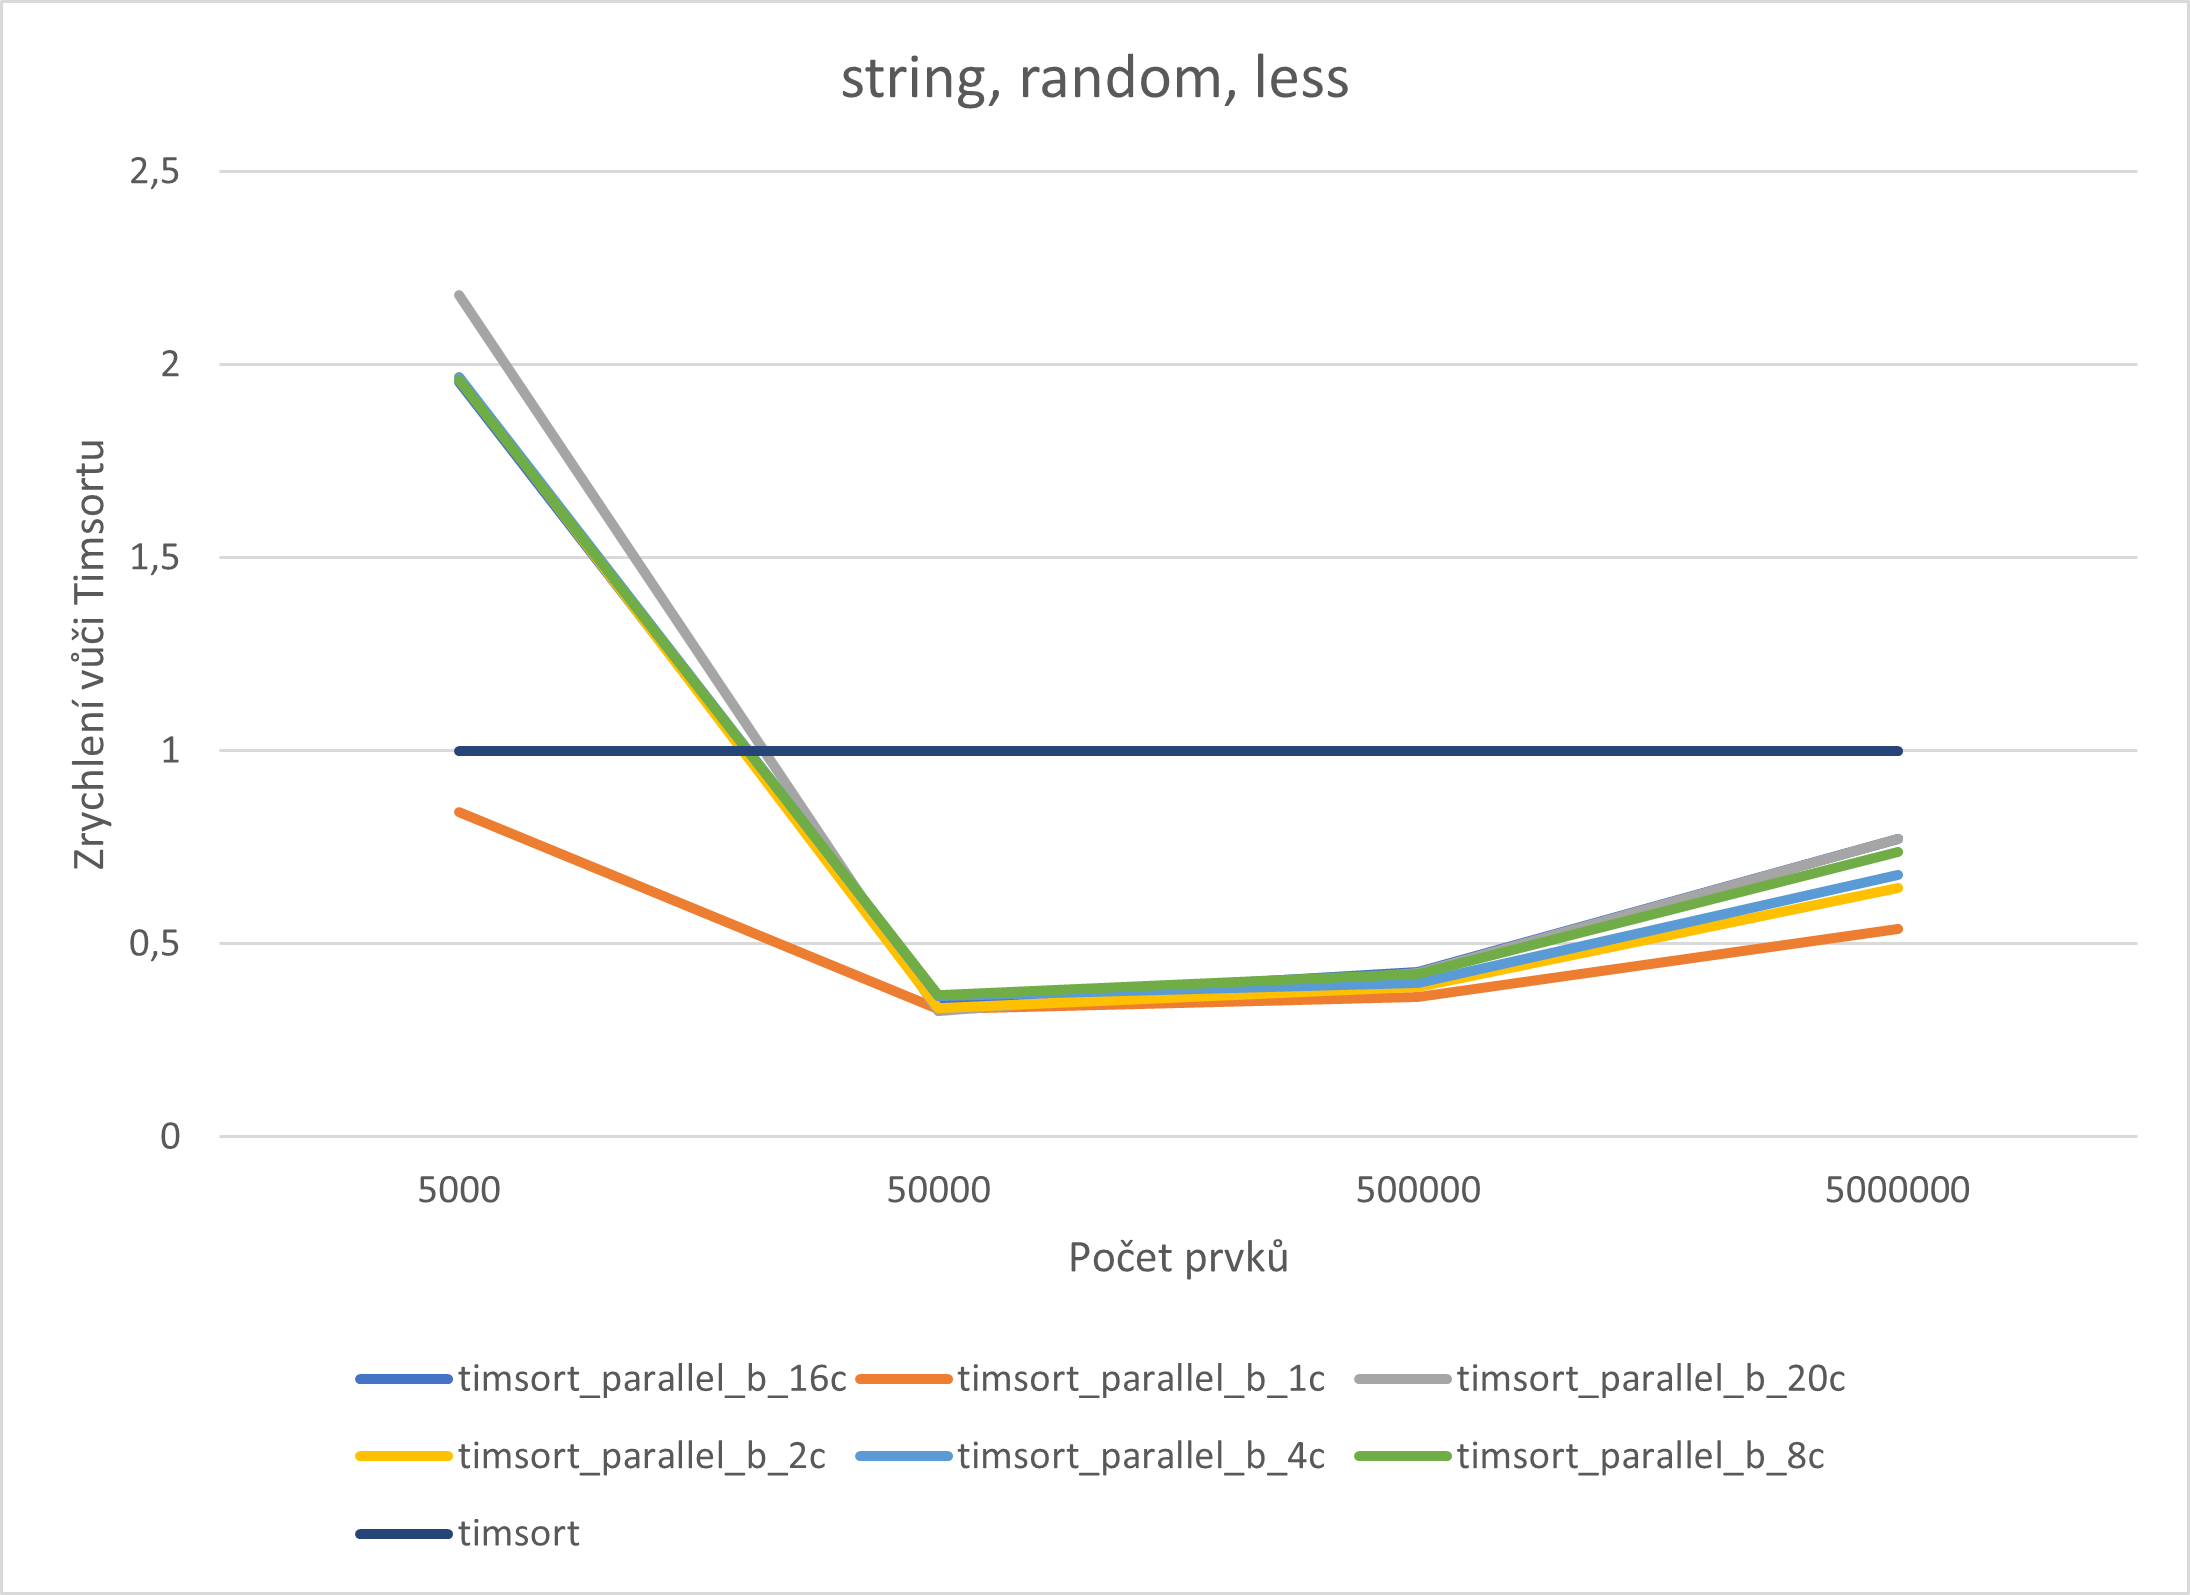
\includegraphics[width=13cm]{obrazky/graf27.png}
	\caption[Zrychlení timsort\_parallel\_b oproti timsortu v závislosti na počtu vláken, náhodné stringy]{Zrychlení timsort\_parallel\_b oproti timsortu v závislosti na počtu vláken, náhodné stringy}\label{fig:graf27}
\end{figure}


Dalším zajímavým testem je pole obsahující několik seřazených posloupností. V tomto testu je totiž \texttt{timsort\_parallel\_b} nejrychlejší, jak můžeme vidět v tabulce \ref{tab:tab5}. Spoustu paralelních algoritmů dopadlo v tomto testu a dalších testech, kde jsou data již seřazená hůře než obyčejný Timsort. To je ovšem očekávané vzhledem k tomu, že paralelní algoritmy předem neví, že data jsou seřazená a zbytečně je rozdělují mezi vlákna. A proto je právě \texttt{timsort\_parallel\_b} v tomto testu nejrychlejší, protože napřed zjistí všechny runy a teprve potom je rozděluje mezi vlákna.

 \begin{table}[htbp]\centering
 	\caption[Porovnání paralelních algoritmů pro pole obsahující několik seřazených posloupností]{Porovnání paralelních algoritmů pro pole obsahující několik seřazených posloupností}\label{tab:tab5}
 	\begin{tabular}{|c|c|}\hline \hline
 		Algoritmus		& zrychlení vůči Timsortu \tabularnewline \hline \hline
merge\_sort\_parallel\_a\_16c & 0,7932\tabularnewline \hline
merge\_sort\_parallel\_a\_1c & 0,1958\tabularnewline \hline
merge\_sort\_parallel\_a\_20c & 0,8578\tabularnewline \hline
merge\_sort\_parallel\_a\_2c & 0,2764\tabularnewline \hline
merge\_sort\_parallel\_a\_4c & 0,3928\tabularnewline \hline
merge\_sort\_parallel\_a\_8c & 0,5654\tabularnewline \hline
merge\_sort\_parallel\_b\_16c & 1,0822\tabularnewline \hline
merge\_sort\_parallel\_b\_1c & 0,3845\tabularnewline \hline
merge\_sort\_parallel\_b\_20c & 1,0725\tabularnewline \hline
merge\_sort\_parallel\_b\_2c & 0,5079\tabularnewline \hline
merge\_sort\_parallel\_b\_4c & 0,6301\tabularnewline \hline
merge\_sort\_parallel\_b\_8c & 0,8173\tabularnewline \hline
timsort & 1\tabularnewline \hline
timsort\_parallel\_a\_16c & 0,9348\tabularnewline \hline
timsort\_parallel\_a\_1c & 1,0002\tabularnewline \hline
timsort\_parallel\_a\_20c & 0,9122\tabularnewline \hline
timsort\_parallel\_a\_2c & 0,4768\tabularnewline \hline
timsort\_parallel\_a\_4c & 0,4766\tabularnewline \hline
timsort\_parallel\_a\_8c & 0,9631\tabularnewline \hline
timsort\_parallel\_b\_16c & 1,2668\tabularnewline \hline
timsort\_parallel\_b\_1c & 0,9342\tabularnewline \hline
timsort\_parallel\_b\_20c & 1,1616\tabularnewline \hline
timsort\_parallel\_b\_2c & 1,1932\tabularnewline \hline
timsort\_parallel\_b\_4c & 1,3018\tabularnewline \hline
timsort\_parallel\_b\_8c & 1,2303\tabularnewline \hline




	\end{tabular}
\end{table}
Také bych zmínil, že vylepšení paralelního mergesortu pomocí slučovací funkce z Timsortu opravdu zafungovalo. Při náhodných datech je zpomalení minimální a při seřazených datech je algoritmus znatelně rychlejší. To ostatně můžeme vidět v grafech \ref{fig:graf28}, \ref{fig:graf29}, \ref{fig:graf30}, \ref{fig:graf31}, \ref{fig:graf32}, kdy při porovnávání výsledků těchto algoritmů lze vidět jasné zrychlení. Mezi těmito grafy lze také porovnat zrychlení pro různý počet vláken. Doba běhu je opět v logaritmickém měřítku a rozdíl jednoho řádku tedy znamená 10-krát zrychlený algoritmus.

\begin{figure}[htbp]\centering
	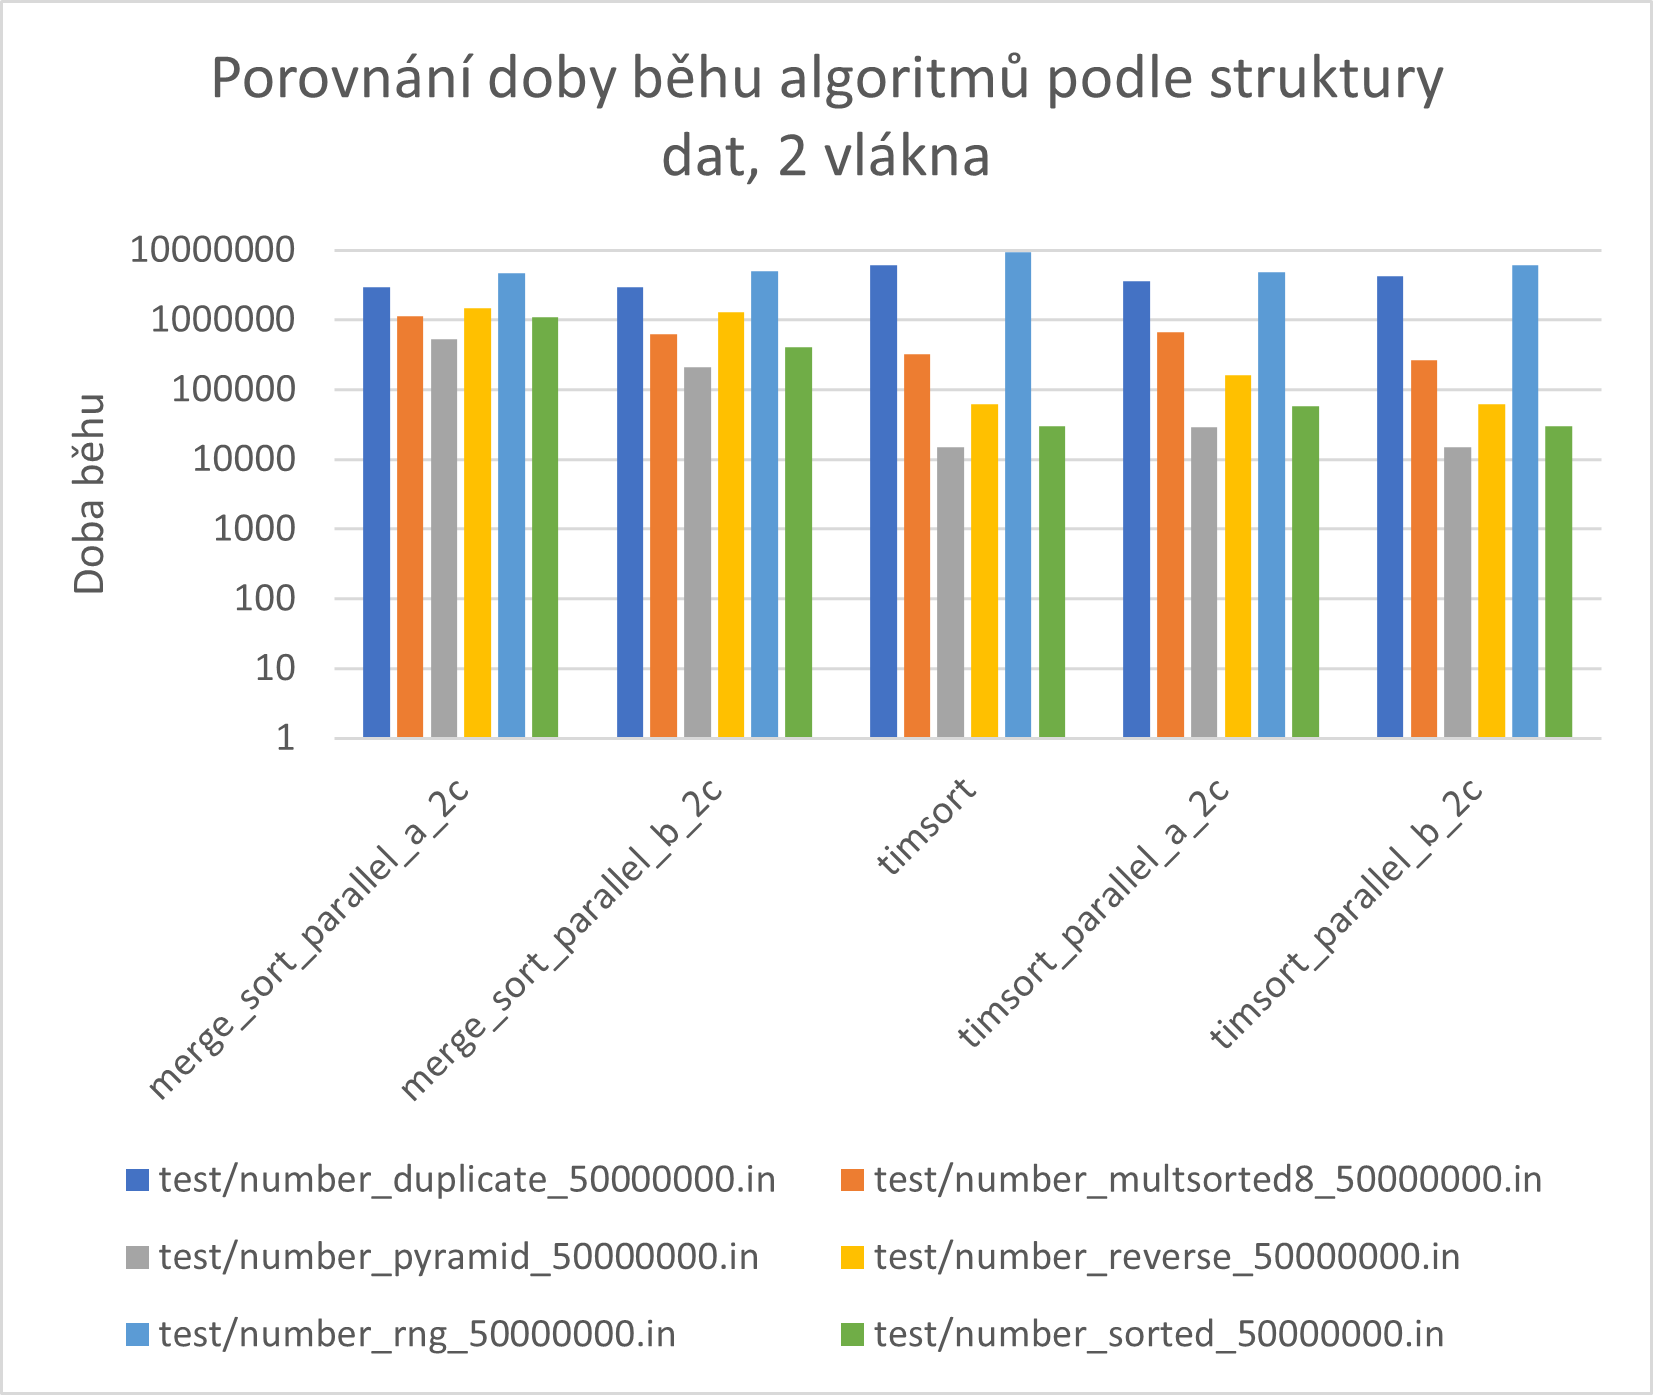
\includegraphics[width=13cm]{obrazky/graf28.png}
	\caption[Porovnání doby běhu algoritmů pro 2 vlákna a různá data o stejné velikosti]{Porovnání doby běhu algoritmů pro 2 vlákna a různá data o stejné velikosti}\label{fig:graf28}
\end{figure}

\begin{figure}[htbp]\centering
	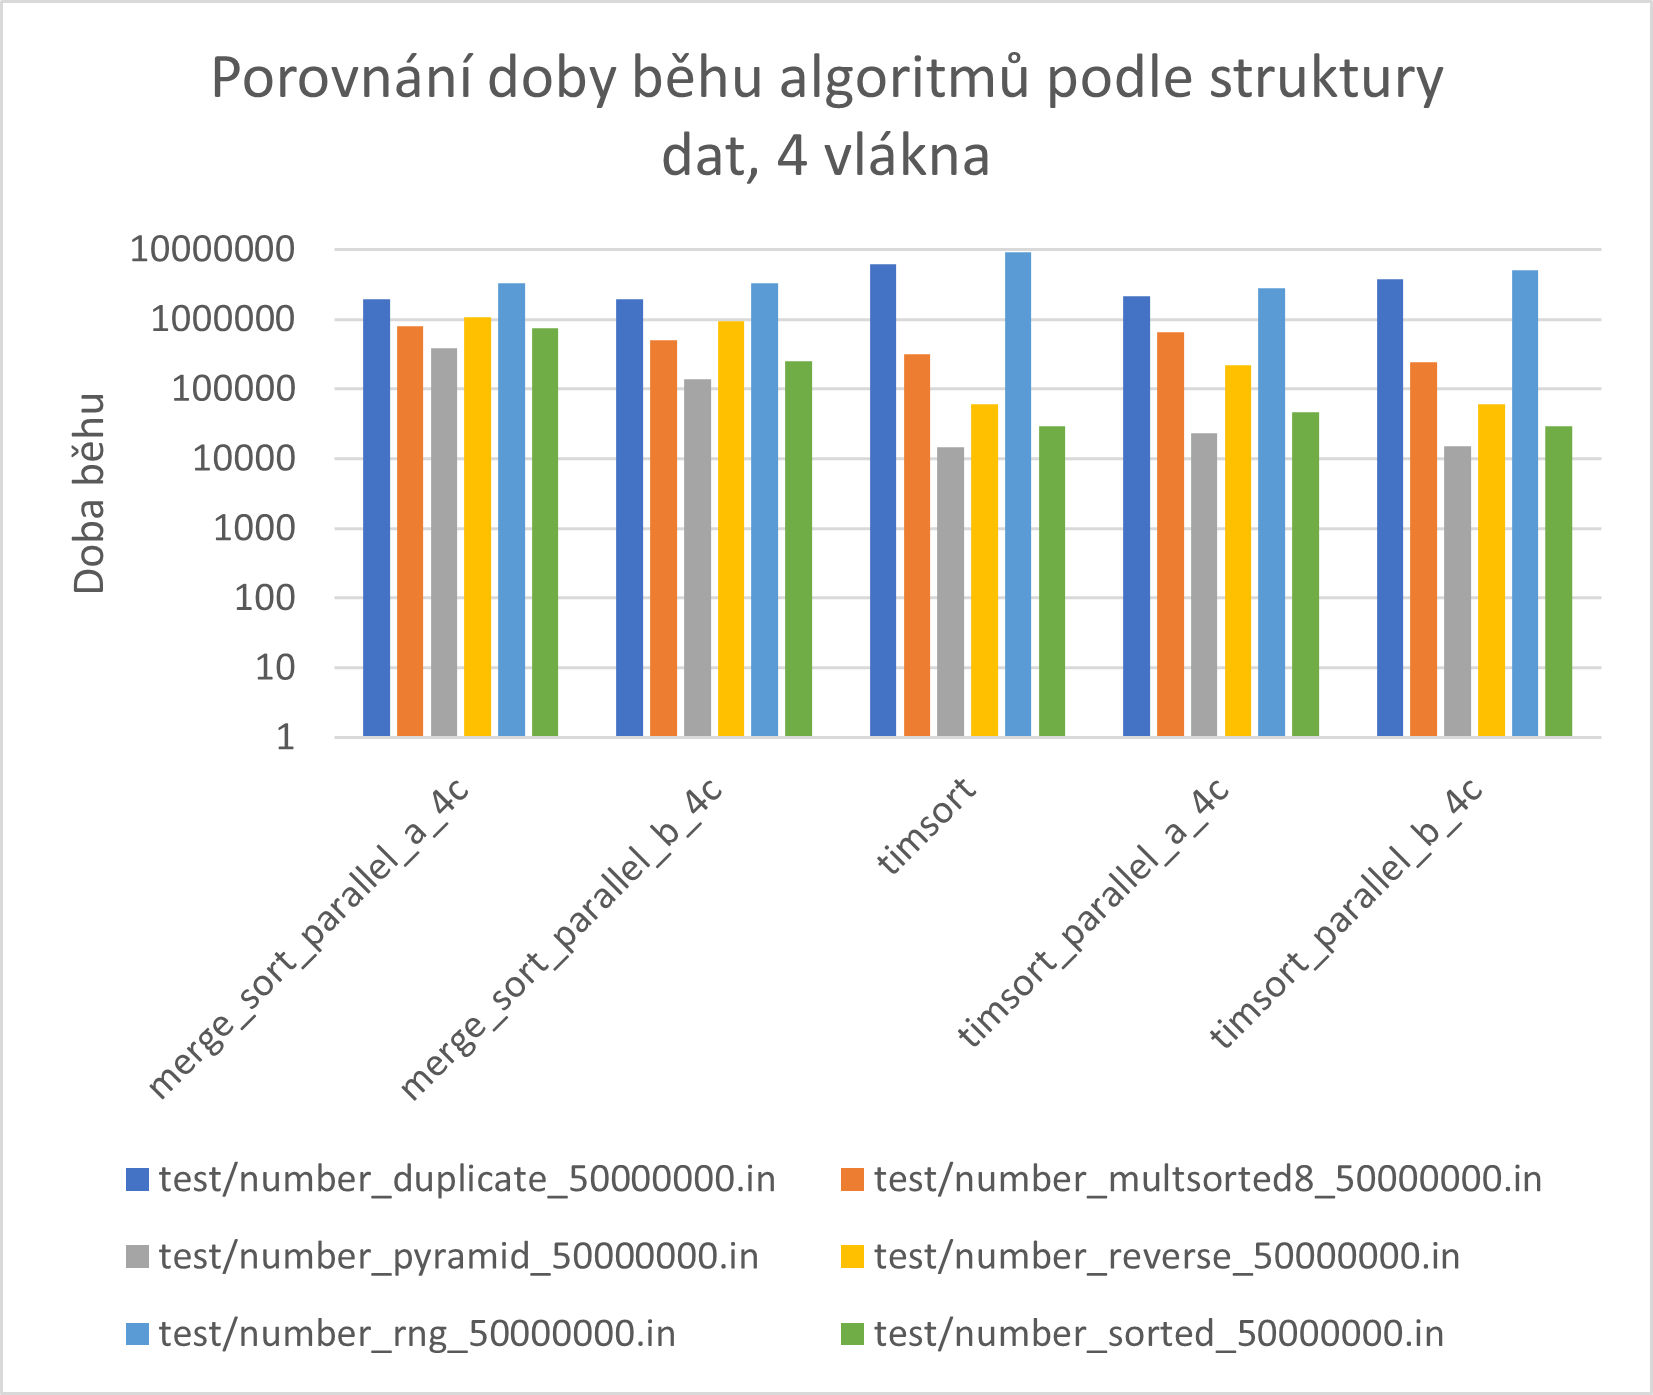
\includegraphics[width=13cm]{obrazky/graf29.png}
	\caption[Porovnání doby běhu algoritmů pro 4 vlákna a různá data o stejné velikosti]{Porovnání doby běhu algoritmů pro 4 vlákna a různá data o stejné velikosti}\label{fig:graf29}
\end{figure}

\begin{figure}[htbp]\centering
	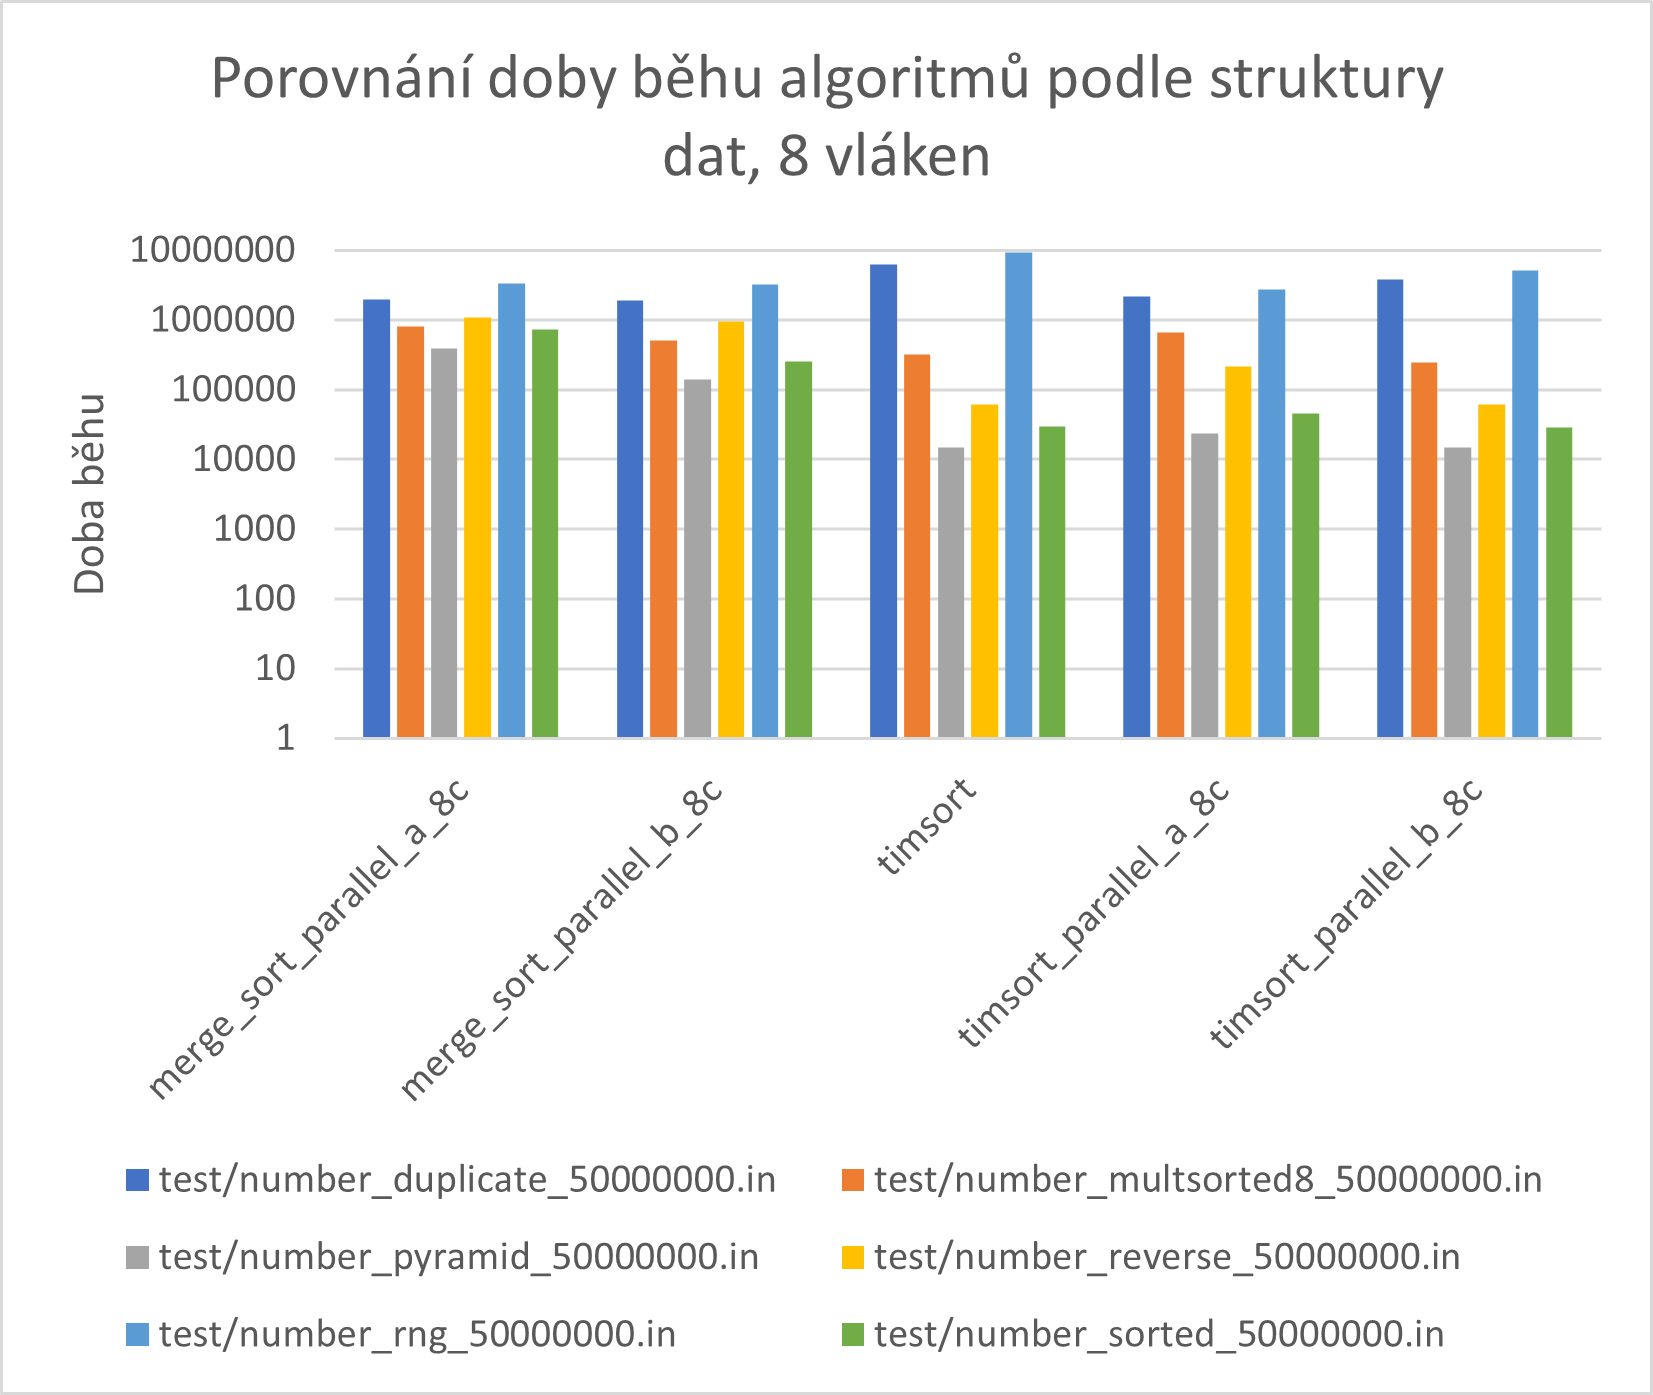
\includegraphics[width=13cm]{obrazky/graf30.png}
	\caption[Porovnání doby běhu algoritmů pro 8 vláken a různá data o stejné velikosti]{Porovnání doby běhu algoritmů pro 8 vláken a různá data o stejné velikosti}\label{fig:graf30}
\end{figure}

\begin{figure}[htbp]\centering
	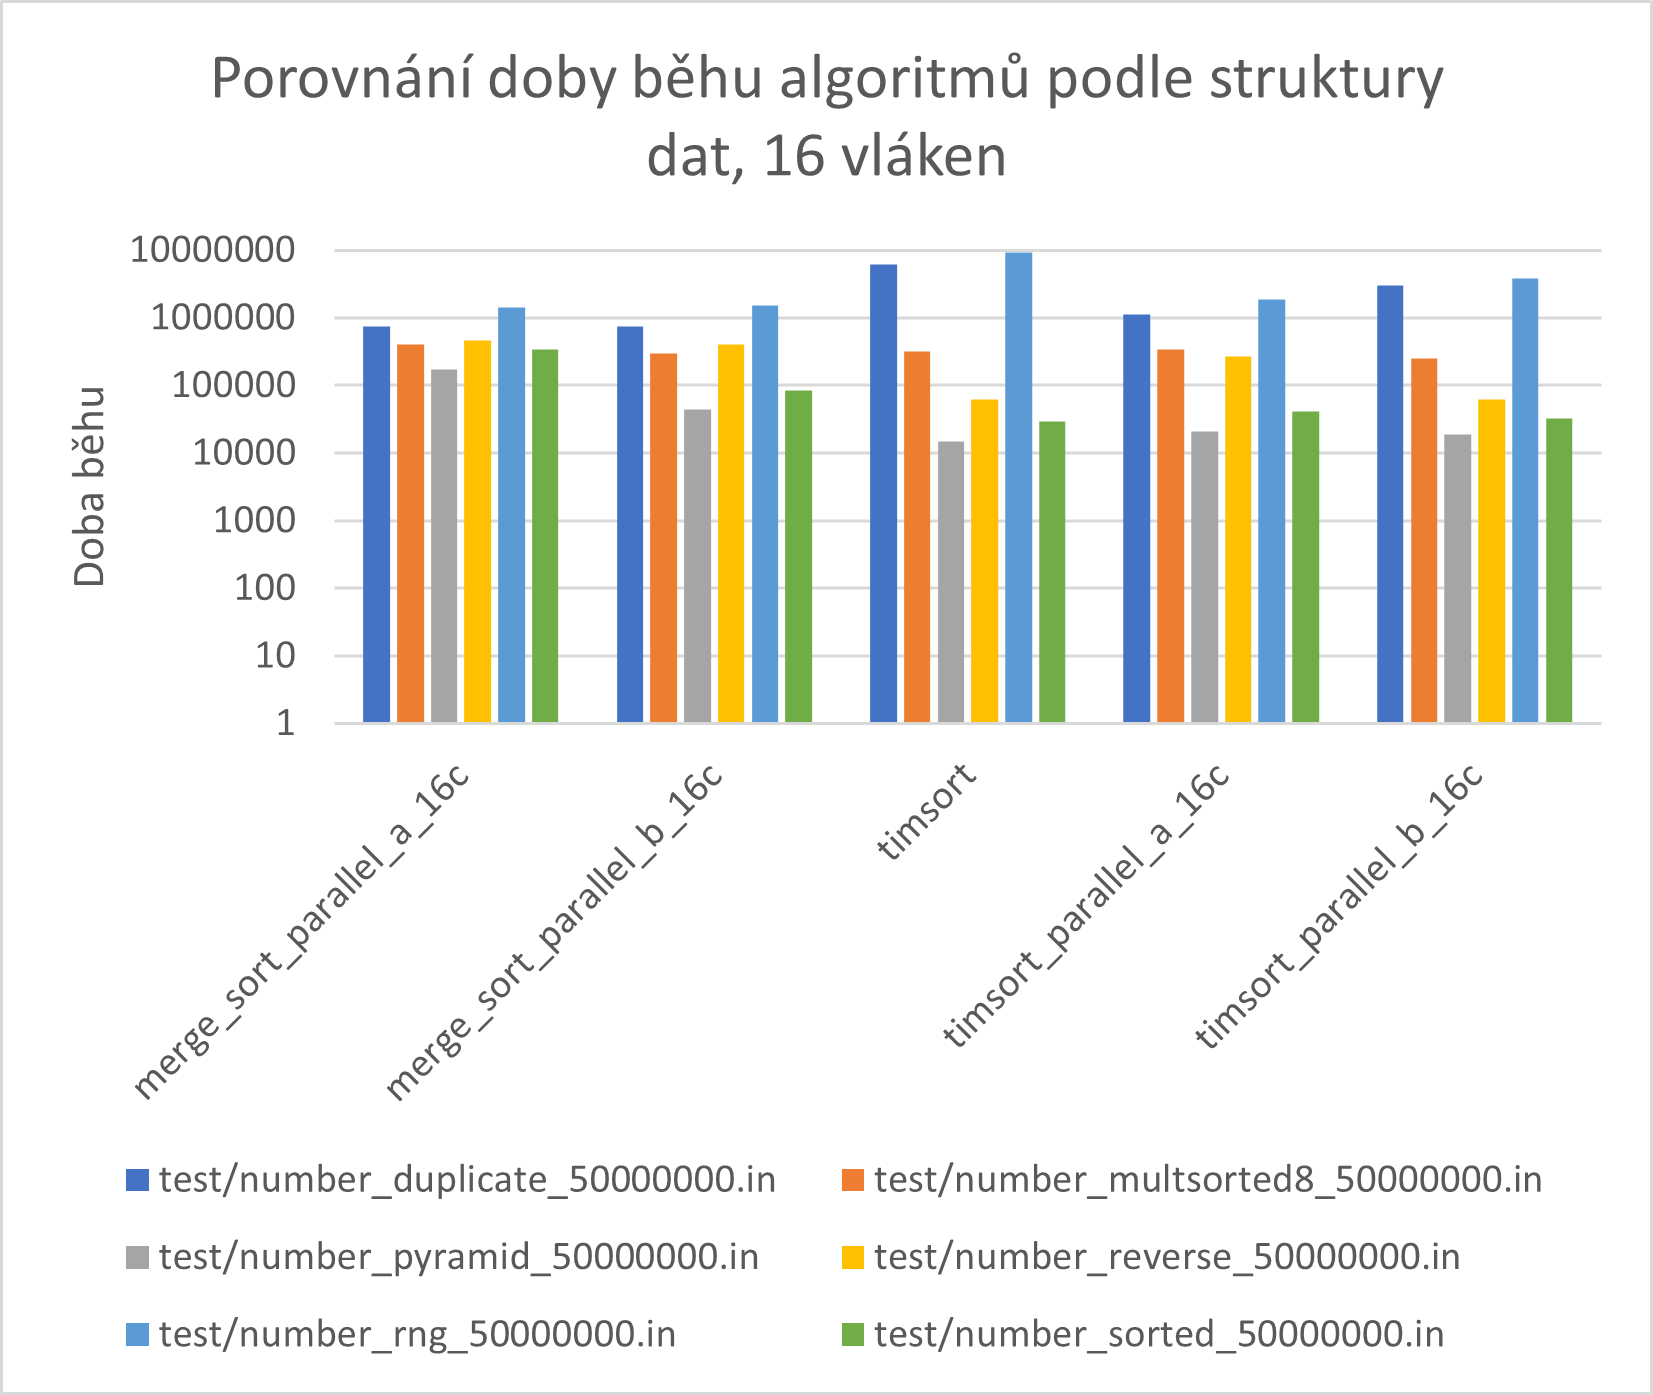
\includegraphics[width=13cm]{obrazky/graf31.png}
	\caption[Porovnání doby běhu algoritmů pro 16 vláken a různá data o stejné velikosti]{Porovnání doby běhu algoritmů pro 16 vláken a různá data o stejné velikosti}\label{fig:graf31}
\end{figure}

\begin{figure}[htbp]\centering
	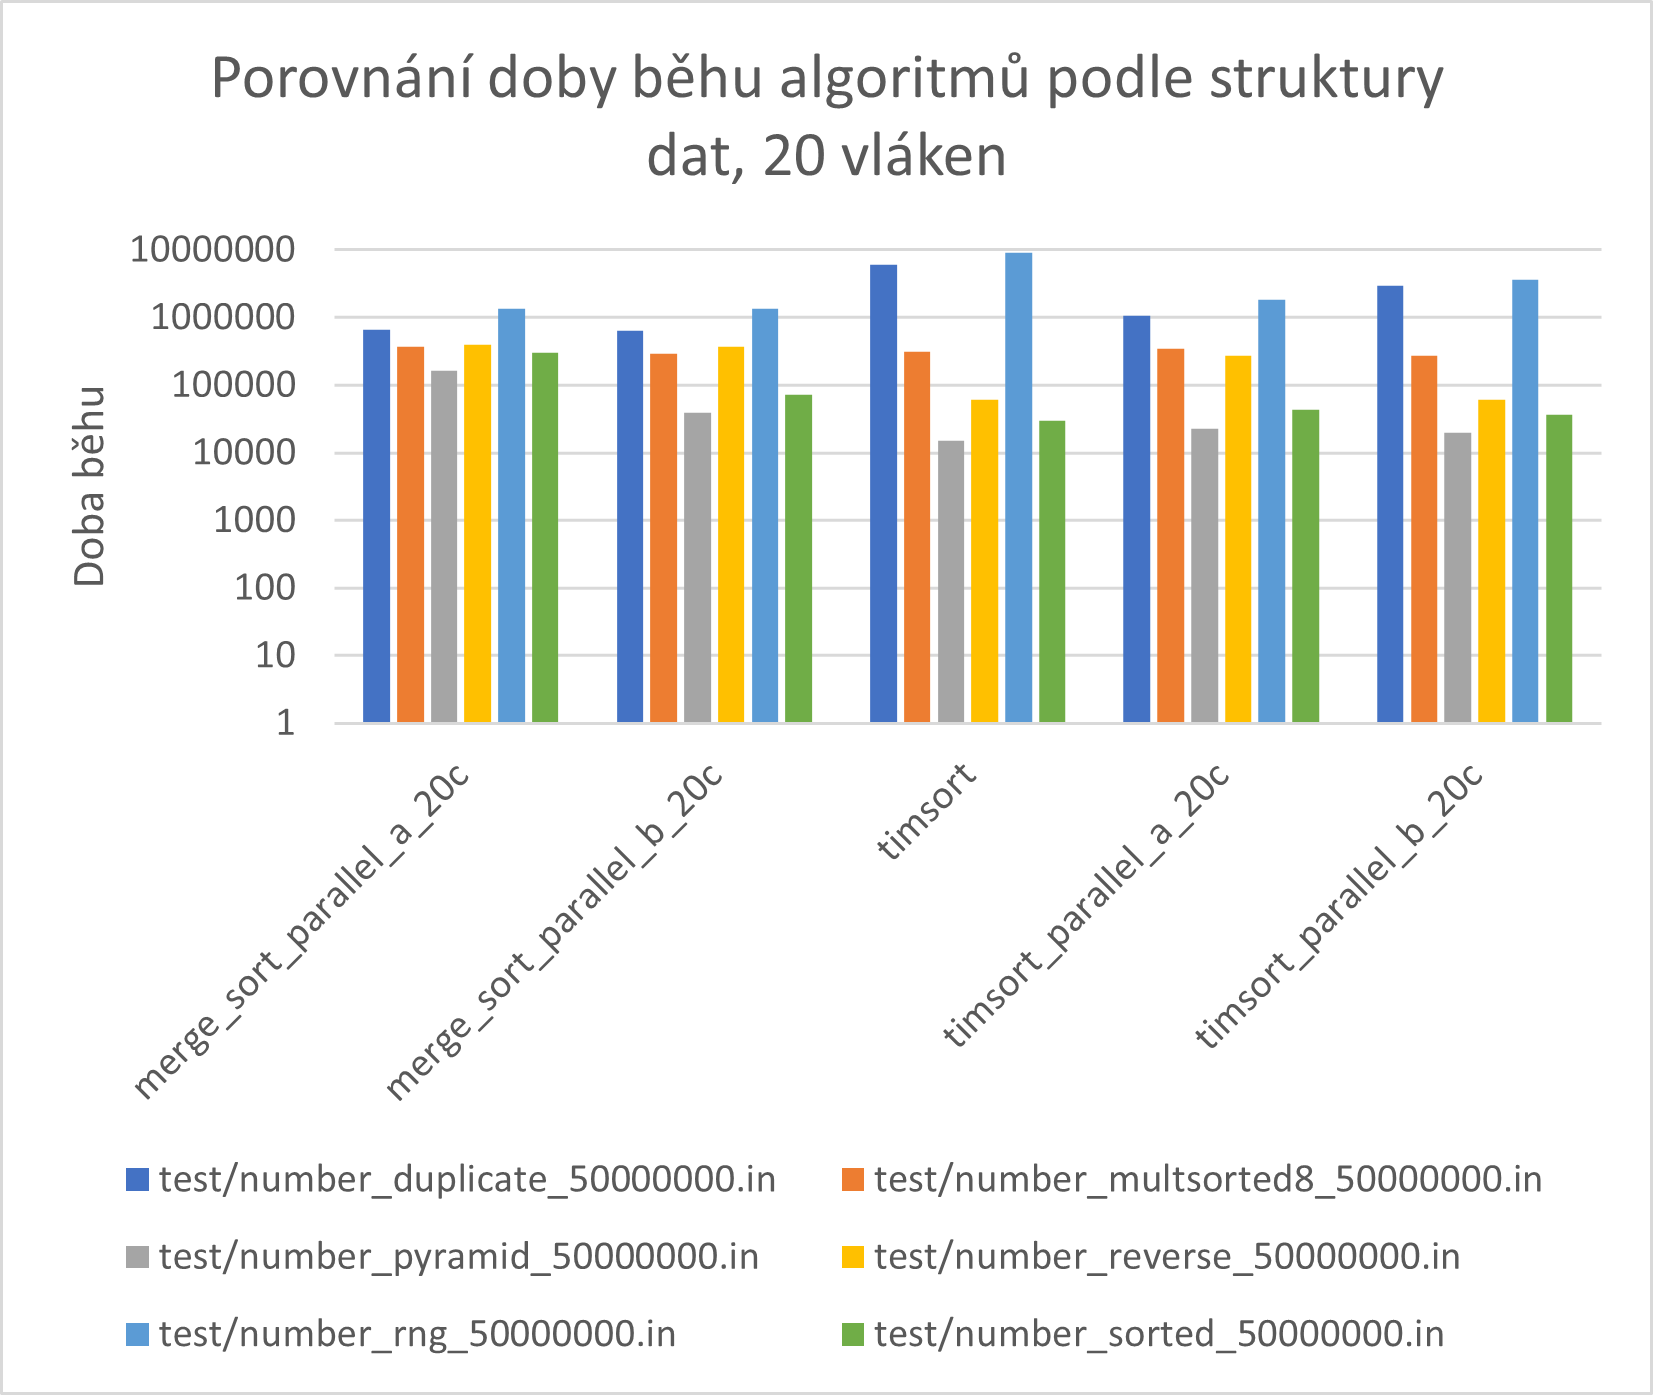
\includegraphics[width=13cm]{obrazky/graf32.png}
	\caption[Porovnání doby běhu algoritmů pro 20 vláken a různá data o stejné velikosti]{Porovnání doby běhu algoritmů pro 20 vláken a různá data o stejné velikosti}\label{fig:graf32}
\end{figure}

\begin{conclusion}
	Prvním cílem této práce bylo studium a implementace algoritmu Timsort. Výstupem této části je funkční řadící algoritmus. Následným testováním jsme zjistili, že jeho chování odpovídá očekávání a chová se stejně jako Timsort z knihovny gfx.
	
	Dalšími body zadání byl návrh optimalizací a paralelizací a jejich následná implementace. Vymyslel jsem proto několik možných sekvenčních optimalizací. Ty zahrnovaly hledání runů od konce pole a slučování více runů najednou. Dále jsem navrhl několik možností paralelizace algoritmu Timsort a vybrané z nich jsem implementoval. Aby byla paralelizace možná, bylo nutné vzdát se některých principů Timsortu a tím jsme přišli o zejména paměťové výhody. Paralelizace ovšem byla úspěšná a zjistili jsme, že každý paralelní algoritmus se hodí na jiný typ dat. To obecně platilo i u sekvenčních algoritmů.
	
	Posledním bodem zadání je porovnání jednotlivých verzí algoritmu na serveru STAR. Ačkoliv testování bylo poměrně obsáhlé, objevil jsem během něj místa, které by bylo vhodné prozkoumat dále do hloubky. Narazil jsem například i na zajímavý bug s řadící funkcí less při řazení stringů. Na všechny detaily testování by nebylo v této práci místo a zmínil jsem proto pouze ty nejdůležitější a největší rozdíly mezi jednotlivými algoritmy. Ověřil jsem, že je skutečně výhodné používat Timsort jako univerzální řadící algoritmus, neboť není o tolik pomalejší při náhodných datech a zároveň je extrémně rychlý při řazení dat obsahující struktury. Zároveň používá méně porovnávacích funkcí a je tedy vhodný, pokud jsou tyto funkce pomalé. Také jsem zjistil, že paralelizovat Timsort má smysl a můžeme tím dosáhnout výrazného zrychlení řazení.
	
	Při diskuzi výsledků jsem navrhoval, s jakými daty šly jednotlivé algoritmy využít a při jakých datech by bylo lepší volit jiný řadící algoritmus. Diskutoval jsem také možnosti využití mnou navržených optimalizací Timsortu. Došel jsem k závěru, že opět záleží na datech, která budeme řadit. Navržené optimalizace mohou algoritmus zrychlit v jednom případě a zpomalit ve druhém. Navíc bychom mohli zase přijít o paměťové úspory Timsortu oproti běžným slučovacím algoritmům.
	
	Na tuto práci lze navázat například pokračováním testování různých dat či porovnávacích funkcí. Dále na ní lze navázat použitím zde zmíněných optimalizací a paralelizací a zkusit je aplikovat na další algoritmy.
	
\end{conclusion}

% \bibliographystyle{csn690}
% \bibliography{mybibliographyfile}

\printbibliography

\appendix

\chapter{Seznam použitých zkratek}
% \printglossaries 
\begin{description}
	\item[RAM] Random Access Memory
	\item[SGE] Sun Grid Engine
\end{description}



\chapter{Obsah přiloženého CD}



\begin{figure}
	\dirtree{%
		.1 readme.txt\DTcomment{stručný popis obsahu CD}.
		.1 exe\DTcomment{adresář se spustitelnou formou implementace}.
		.1 src.
		.2 impl\DTcomment{zdrojové kódy implementace}.
		.2 thesis\DTcomment{zdrojová forma práce ve formátu \LaTeX{}}.
		.1 text\DTcomment{text práce}.
		.2 thesis.pdf\DTcomment{text práce ve formátu PDF}.
		.1 results\DTcomment{výsledky testování použity v této práci}.
	}
\end{figure}

\end{document}
